\documentclass[11pt,a4paper]{report}


%%% packages

  \usepackage{a4wide}           % set page size etc

  \usepackage{graphicx}  % to include figures in .eps-format
  \usepackage{multido}          % used in chapter 3 to repeat text
  \usepackage{setspace}         % provides \onehalfspacing
  \usepackage{url}              % to set URLs, paths, commands ... in tt
  \usepackage{amstext}          % provides \text, which, unlike \mbox, scales
  \usepackage{amsmath}          % provides align and align*, besides others
  \usepackage{times}            % switches to the Times font, saves space
  \usepackage{amssymb,mathptmx} % provides more math symbols
  \usepackage{float}
  \usepackage{parskip}
  \usepackage{enumitem}
\setlist{noitemsep,topsep=0pt,parsep=0pt,partopsep=0pt}
\usepackage[compact]{titlesec}
\usepackage{rotating}

%%% new commands
  
  \newcommand{\PD}[2]{\frac{\partial #1}{\partial #2}} % partial derivation
  \newcommand{\dd}{\,\mathrm{d}} % to be used in differentials

% Rules for handling pre-zipped figures. To create zipped figs do this:
% $ head myfigure.eps > myfigure.eps.bb
% $ gzip myfigure.eps
  \DeclareGraphicsRule{.eps.gz}{eps}{.eps.bb}{`zcat #1}
  \DeclareGraphicsRule{.epsi.gz}{eps}{.epsi.bb}{`zcat #1}
  \DeclareGraphicsRule{.eps.Z}{eps}{.eps.bb}{`zcat #1}

%%% One and a half line spacing

% \renewcommand{\baselinestretch}{1.5}
  \onehalfspacing % better than \renewcommand{\baselinestretch}{1.5}


%%% other styles

  \setcounter{secnumdepth}{3}
  \setcounter{tocdepth}{4}

 

\begin{document}

\thispagestyle{empty}

\vspace*{73.5mm}
\begin{center}
  \setlength{\unitlength}{1mm}
  \begin{picture}(110,60)
    \put(-1,0){\makebox(110,60){% 1mm off the centre to match the hole
        \begin{minipage}{110mm}%% in the lime green card board cover
          \begin{center} \Large
            \textbf{An Evaluation of OpenStack} \\
            {Conor Sloan} \\
            {Computer Science} \\
            {2013/2014}             
          \end{center}
        \end{minipage}
      }}
    \put(54,30){\oval(110,60)}% 1mm off the centre too
  \end{picture}
\end{center}
\vspace*{\fill}

\noindent 
The candidate confirms that the work submitted is their own and the
appropriate credit has been given where reference has been made to the
work of others.

\quad

\noindent 
I understand that failure to attribute material which is obtained from 
another source may be considered as plagiarism.

\quad

\begin{flushright}
  (Signature of student)\underline{\hspace*{2in}}
\end{flushright}

          % This is the front page

\pagestyle{plain}        
\pagenumbering{roman}    % Set up page numbering
\setcounter{page}{1}

\begin{center}
    {\LARGE\bf Summary}
\end{center}

This project involves researching into the various features and characteristics of the OpenStack technology, via a number of different approaches, including research analysis \& both manual and automated experimentation, in order to provide an Evaluation of the technology for the upcoming EU project ASCETiC\cite{ascetic}. \\ \\ This 'Evaluation' of OpenStack will hope to achieve a greater insight to its workings, providing a guide by which to effectively utilise its features whilst avoiding its potential pitfalls and difficulties. It will also provide validation for a lot of key functionality, as a way of determining whether use of OpenStack in a project is justified, along with a review of the various use cases of OpenStack, in order to assess it's viability in the current market. In order to achieve these aims, a simple experiment based model will be used, with logs and conclusions of these experiments forming the bulk of the 'evaluation'. A high level research approach will be used in conjunction with this to give a good overview of the technology. \\ \\ 
The deliverables for this project include a report detailing my approach to evaluating OpenStack, as well as a number of designed experiments with results and logs attached, including my own reflection and conclusions on what these results represent. As a secondary objective, this project aims to provide re-usable software tools and components, such as libraries and  scripts, for the effective use of OpenStack in future. 



        % Summary
\begin{center}
    {\LARGE\bf Acknowledgements}
\end{center}

Firstly, I would like to thank my project supervisor, Karim Djemame, for his unwavering support, guidance and patience, especially in times where circumstance made project progress difficult. This project would have been very difficult without his knowledge and experience. \\

Secondly, my thanks to Django Armstrong, who, despite having a very busy schedule, took the time to deploy OpenStack on the TestBed on behalf of my project, and was consistently responsive and helpful whenever there were technical issues concerning the deployment. \\

I would also like to thank David Duke, my assessor, whose feedback and guidance from my mid-project report and organised assessor meeting were invaluable in uncovering the real aims and identity of this project.  
% \newpage

    % Acknowledgements
\tableofcontents
\newpage

\pagenumbering{arabic}   % Set up page numbering
\setcounter{page}{1}

\chapter{Introduction}
\label{CHAP_FIRST}
\centerline{\rule{149mm}{.02in}}
\vspace{2cm}

This section will outline an introduction to the project, discussing a number of different topics such as: 

\begin{itemize}
\itemsep0em
  \item The chosen domain and involved technologies
  \item The motives and justification behind the project
  \item The Aims and Objectives of the project
  \item The chosen approach to the execution of the project
  \item The Project Plan going forward
\end{itemize}

Hopefully, these explanations will give some context to the work being done, answering such questions as "Why this project?" and "What value does this work bring?"

\section[Overview]{Project Overview}

I chose to pursue this project for a number of reasons. Firstly, Cloud Computing is an area of technology which I have great interest in, having worked with similar technologies in previous employment and in personal projects. Secondly, and perhaps more importantly, is the incredible rise of the Cloud to prominence in the Computing industry in recent years, with the Infrastructure as a Service (IaaS) model at the forefront. The emergence of public clouds from tech giants such as Amazon and Microsoft has lead to a huge increase in the popularity of related software technologies, usually Virtual Infrastructure Managers using Virtualisation technology to service clients' computing needs in an on-demand manner. \\ 
Amongst the many current solutions out there, one technology in particular has grown in popularity to the point that it is fast becoming the de facto open source standard for IaaS clouds. This technology is OpenStack. 
This popularity makes OpenStack a perfect candidate to be assessed in terms of its capabilities and characteristics; in short, we want to know  \textit{why} OpenStack is becoming so popular, and if this popularity is justified.  
In order to answer this question, my work will involve researching into the relevant areas of Cloud Computing, Data Centre Virtualisation and Web Services, and performing qualitative and quantitative assessment of OpenStack through various approaches and experiments. 

\subsection{Project Aims and Justification}

There are a number of aims to this project. Firstly, I aim to research the area of Infrastructure as a Service Clouds, including the desirable characteristics and requirements of these clouds from a number of different perspectives, current IaaS market offerings, and what technologies are involved in producing such a solution. This research should culminate in an overview of OpenStack, which technologies it uses, and what it does. Once this background research preparation is complete, my main target will be to produce a critical evaluation of OpenStack, in the form of a report, detailing OpenStack with respect to its functionality and architecture. I also aim to perform both qualitative and quantitative assessment of OpenStack through experiments. These experiments will also be part of my deliverable, and should serve as documentation of how to use OpenStack, and provide re-usable software to test the functionality of OpenStack. The results of these experiments will be used as evaluation. Finally, I will analyse my results and approach to evaluation of OpenStack, and ask a number of questions concerning how well my performance covers the technology, how reliable my results are, and what impact my evaluation actually has. This evaluation of my evaluation will serve as another deliverable, giving an assessment of the advantages and disadvantages of my approach in retrospect.  \\ 
I consider this project to be worthwhile mainly due to the importance of OpenStack, considering its relative infancy in the market compared to it's competitors. This product is becoming increasingly dominant, and yet was only released in 2010 \cite{Piatt10}, so much less is known about it than many other solutions. For this reason, I believe an analysis of the product is worthwhile. Secondly, this project serves as a precursor for an EU project, ASCETiC \cite{ascetic}, which the School of Computing will be involved with; The knowledge and guides provided by this project could be very helpful in the workings of the project. This backing alone justifies the idea of getting to know OpenStack better. 

\subsection{Objectives}

Formally, my objectives are as follows:
\begin{itemize}

\item \underline{Produce a Literature Review of relevant source material}: A background research report, starting with Cloud Computing as a whole, with particular focus on public clouds, virtualisation, IaaS and the current IaaS market, and of course, OpenStack. The idea behind this is to give context to the reader and introduce them to the various technologies and concepts involved in this project. 

\item \underline{Produce an Evaluation Report of OpenStack}: The main deliverable of this project, the report will provide guides of how to use OpenStack, useful for future projects, as well as providing insight as to the workings of OpenStack via Qualitative \& Quantitative assessment. The report will draw conclusions about OpenStack as a whole, and give some idea of whether it is a good idea to use it. 

\item \underline{Produce a number of designed experiments and results to assess OpenStack functionality}: will be varied, so as to assess OpenStack in a number of different ways. The experiments should be designed, implemented, and then executed, with results and derived conclusions attached. They will serve as a source of information for the Evaluation report. 

\item \underline{Produce Implementations for a number of programmatic tests of OpenStack}: This objective is closely linked to the previous objective. Some experiments will be programmatic tests written using the various RESTful Web Services provided by OpenStack. These should be able to be reused given a different endpoint for the Web Service Client, and so full implementations of these should be provided as a deliverable. They will also be used to validate OpenStack functionality. 

\item \underline{Produce re-usable software components for use of OpenStack}: Similarly to the previous objective, a set of software tools should be produced as part of this project, which will allow others to easily interact with OpenStack in the same way this project has for experiments. This will most likely be a Java tool, providing access to OpenStack's APIs. 

\item \underline{Produce an evaluation of my approach to evaluating OpenStack}: The final objective is to provide some evaluation of my work. This is a way of comparing my evaluation with others that are out there, and assessing the successes and shortcomings of my approach and work. I will discuss how I may have improved my approach in this part of the report, and how this would have improved the outcome. I will also assess the quality of my deliverables.   

\end{itemize}

\subsection{Minimum Requirements}

The minimum requirements of this project to achieve a pass are as follows:
\begin{itemize}
\itemsep0em

\item Provide a \underline{basic literature review} of Cloud Computing, Virtualisation, IaaS and OpenStack. 
\item Provide at least 1-3 repeatable \underline{designed experiments} to assess the functionality of OpenStack, with logs and results. 
\item Provide code for at least one \underline{programmatic experiment} to assess the functionality of OpenStack, with source code, logs and results. 
\item Provide an \underline{Evaluation Report} of OpenStack containing Qualitative Assessment of its features. 
\item Provide at least one \underline{re-usable software component} for OpenStack. 
\item Produce an \underline{Evaluation} of the project approach. 

\end{itemize}

\subsection{Possible Extensions}

There are a number of possible extensions to this project which could be performed if there is enough time. These are extensions that are not expected to be completed, and are beyond even exceeding the minimum requirements, and achieving all of the stated objectives. Extensions are listed below:
\begin{itemize}
\itemsep0em
\item \underline{Comparison with another product} - deploy an alternative cloud computing platform, in order to gain perspective particularly with respect to quantitative results. 
\item \underline{Different OpenStack configurations} - perform experiments with a number of different OpenStack setups; 
\item \underline{Produce an experiment/test framework} - provide some reusable code to create new experiments for OpenStack; this could just be a set of commonly used utilities, or a fully blown programming/testing framework. 
\end{itemize}

\subsection{Deliverables}

These are the deliverables of the project, based on the minimum requirements. 
\begin{itemize}
\itemsep0em
\item \underline{An Evaluation Report} - detailing strengths and weaknesses of OpenStack
\item \underline{Designed Experiments} - with descriptions, targeting functionality of OpenStack
\item \underline{Logs \& Results} - From aforementioned experiments, including code from programmatic tests. 
\item \underline{Re-usable software components} - For future interaction with OpenStack, could be scripts, programming libraries, etc.
\item \underline{Evaluation} - Of the project approach, where it succeeded and failed, and other critical points.
\end{itemize}

\section{Methodology}
\subsection{Project}
In order to achieve the objectives set for this project, work will be split into 4 key areas. These areas are left deliberately wide and high level so as to allow an agile, iterative approach to development. The key reason for this approach is my inexperience with the software and technologies involved, and the time constraints. It is likely that much learning of OpenStack will commence whilst the experiments are being developed, and this new knowledge could have an effect on how the experiments are written. For this reason, a traditional waterfall model with clearly separated stages such as 'design' and 'implementation' would not be ideal. \\
The three steps are as follows:
\begin{enumerate}
\itemsep0em
\item \underline{Research Phase} - concerned with laying the ground work of the project, including literature review \& project planning.
\item \underline{Implementation Phase} - covers most of the practical work, stretching from initial design of the experiments to the logging of results from executing those experiments. 
\item \underline{Conclusion phase} - Once all data has been collated and collected, conclusions must be made regarding the work done, and the evaluation itself must be summed up.
\item \underline{Evaluation Phase} - Every stage of the process must be evaluated. This phase is chiefly for writing up this evaluation, as the plan is to constantly evaluate work at each stage of the project. 
\end{enumerate}  
Version control will be used for all code including write up, and tasks will be managed through the use of productivity tools such as note taking applications, and code comments. 

\subsection{Experiment}

Development of experiments will follow an iterative model, allowing for an agile approach. This is mainly due to it being likely that each experiment will adapt and change as I become more comfortable with OpenStack, and with the technologies involved. If experiments have some practical element, e.g. programming, and require development of some deliverable, they will roughly follow an agile design-implement-test cycle, until the results are deemed reliable. Development will happen mostly in 'sprints' bursts of work with dedicated outcome objectives.\\
In terms of the types of experiment, a mixed approach of Quantitative and Qualitative experiments are likely to be developed. Qualitative experiments are those producing qualitative results, i.e. those which cannot be expressed as a number\cite{qualquantdef}. For example, when comparing features, whether OpenStack has a feature is qualitative. Quantitative experiments are those producing quantitative results, i.e. those which can be quantified, or expressed as a number\cite{qualquantdef}. For example, performance tests of a task with OpenStack may give numerical time results - these are quantitative. \\
Combining these two approaches could give a more well-rounded evaluation, based both on its performance and characteristics. This will be elaborated on in the literature review. 

\section{Project Plan}
In this section, the plan for the project will be set out, including the work schedule and the various milestones of the project. This structure is put in place to allow a more methodical and organised approach to the project work. 

\subsection{Schedule}

This project will follow a specific schedule on a weekly basis, proposed in the first week of the project, hopefully allowing for a structured set of goals every week. This of course is difficult to predict in any project, and any changes to the proposed schedule will be discussed in the Evaluation section of this report.  

\subsection{Milestones}

Milestones are important in a project in that they give a good indication on how far along the project is, and set a clear target on when goals should be achieved. These are listed below:

\begin{itemize}
\itemsep0em
\item \underline{Milestone 1} - The minimum requirements \& aims and objectives must be agreed on and delivered in week 2 (7th February 2014). 
\item \underline{Milestone 2} - The literature review first draft must be completed by week 5 (2nd March 2014) to allow for practical work to commence. 
\item \underline{Milestone 3} - The mid-project report must be delivered on 7th March 2014. Some evidence of work with OpenStack must be seen by then. 
\item \underline{Milestone 4} - At least 2 experiments must be designed and executed by week 11 so as to begin writing up the results. 
\item \underline{Milestone 5} - The progress meeting will take place on 30th April 2014. This is a demonstration of the project to supervisor and assessor. 
\item \underline{Milestone 6} - This report must be submitted by 14th May 2014. 

\end{itemize}

\subsection*{GANTT Chart}

An initial GANTT Chart detailing the aforementioned schedule \& milestones is provided, along with a chart of project deadlines, in Appendix F. 

%\begin{figure}[ht]
%\centering
%\fbox{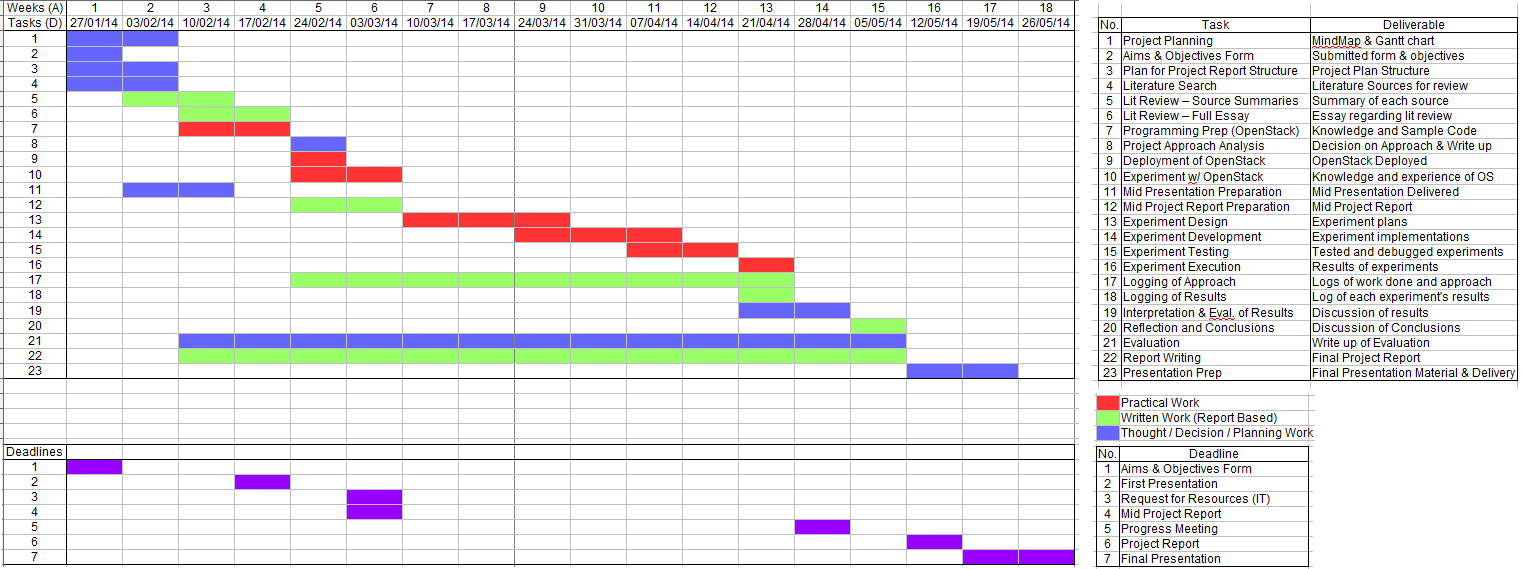
\includegraphics[scale=0.44]{joint-gantts3}}
%\caption{GANTT Chart representing initial project schedule \& Deadlines}
%\end{figure}
\section{Conclusion}

In this section, the fundamental basis of the problem \& subsequent project, as well as the approach to be taken, have been described. Certain aspects of project management have also been covered, to give some idea of how the work will be executed. At this point, the reader should have some idea of what this project is trying to achieve and why, and also some idea of how it will be completed. \\

In the next section, to continue with the 'build up' to the project work, the various aspects of technology which are relevant to the project will be researched and laid out for the reader, in order to build up an understanding of the project domain and its various concepts. The section will also consider, based on the knowledge acquired, how to proceed with an 'Evaluation of OpenStack' beyond a high level project approach.        % include the chapters
\chapter{Background Research}
\label{CHAP_SECOND}
\centerline{\rule{149mm}{.02in}}
\vspace{2cm}

\section{Overview}
This section will introduce the key concepts and technologies involved with this project, starting from a very high level and moving into specialised areas more relevant to OpenStack. The aim here is to give some context to the work that will be done, provide a foundation for the project and allow  the reader to explore further into relevant source material by following the references I provide.\\ 
Once the initial topics have been introduced, I will bring these together and discuss my plan for OpenStack, including critically assessing some existing papers with the same aim, so as to improve upon them and provide a better solution.

\section{Cloud Computing}
\subsection{Introduction}
Cloud Computing is an area of computing which is very high level, and so difficult to precisely define. It's increase in popularity in recent years have seen it come to the forefront of Computing Technology, and this trend is likely to continue for many years. Many companies now offer 'Cloud Solutions' such as Amazon's Amazon Web Services (AWS) \cite{awsec2} and Microsoft's Windows Azure \cite{winazure}. \\ 
In this part of the research, topics considered include the definition of Cloud Computing, its history and the evolution of the cloud industry. Also covered are the different forms of Cloud Computing services, and some real world applications of Cloud Computing.  

\subsection{Definition}
There are many different definitions of Cloud Computing \cite{21definitions}, each giving some insight to the perspective of the person or organisation coining the definition. The National Institute of Standards and Technology (NIST), for example, defines Cloud Computing as: "\textit{a model for enabling ubiquitous, convenient, on-demand network access to a shared pool of configurable computing resources (e.g., networks, servers, storage, applications, and services) that can be rapidly provisioned and released with minimal management effort or service provider interaction}." \cite{nistcloud} \\
McKinsey \& Co. gave a slightly different definition: “\textit{Clouds are hardware based services offering compute, network, and storage capacity where: Hardware management is highly abstracted from the buyer, buyers incur infrastructure costs as variable OPEN, and infrastructure capacity is highly elastic}” \cite{mickinseyclearingtheair} 
From these definitions, there emerged a number of key common characteristics that define a cloud. Most of these were captured by Armburst et al\cite{armbrustberkeleyview}, and consist of:

\begin{itemize}
\itemsep0em
\item Abstraction - The illusion of infinite resources; Often using Virtualisation. 
\item Pay-per-use - The ability to pay for use as needed;
\item Elimination of start-up commitments by cloud users;
\item Self-service interfaces to reduce necessity of human involvement in process. This is a way of automating cloud management processes. 
\end{itemize} 

The main idea is linked to utility computing, and delivering computing to a consumer as a utility, or as a 'service'\cite{armbrustberkeleyview}. This is a large part of cloud computing will be covered in more detail in other parts of this section. 
Overall, there is no clear definition of Cloud Computing; it appears to be a very high level concept or 'umbrella term' covering on-demand computing services aimed at consumers and businesses.\cite{buyyacloudemerging}.   
 
\subsection{Types of Cloud}
There are a number of different 'types' of cloud, also known as \textbf{Deployment Models}. Each of these has uses and suits a particular situations or needs, and so they successfully co-exist. The three main models, illustrated in the below figure, are public, private and hybrid clouds. 

\begin{figure}[ht]
\centering
\fbox{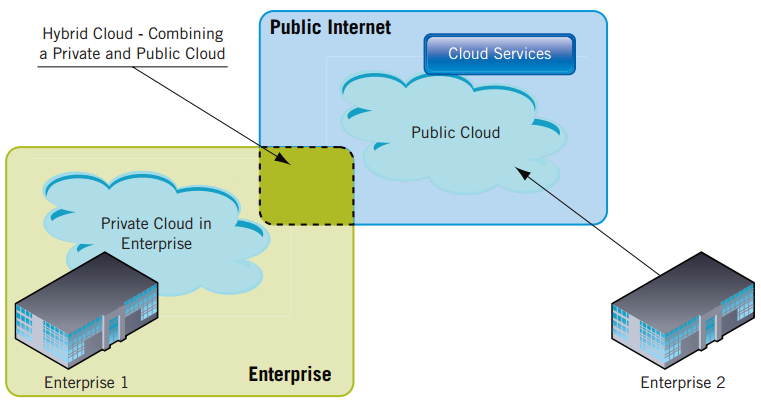
\includegraphics[scale=0.35]{cloud_types}}
\caption[An example figure.]{Cloud Deployment Models \cite{dialogiccloud}.}
\end{figure}

Armbrust et al. \cite{armbrustberkeleyview} define a \textbf{Public Cloud} as a "\textit{cloud made available in a pay-as-you-go manner to the general public}". A Cloud Service Provider (CSP) such as Amazon makes such cloud infrastructures available. This version of a cloud is ideal for start up companies, who may acquire resources without any of the start-up costs associated with developing in-house infrastructure\cite{amazonwhatiscloudcomputing}. Another advantage of a public cloud is the high limit of resources available - using the resources of a global cloud provider gives the potential of enormous elasticity, as they are prepared to service huge demand from a large consumer base. An example of a public cloud service is Google's App Engine, which lets consumers build and run applications on Google's infrastructure, accessed using the internet\cite{googleappengine}. \\ \\
The same publication \cite{armbrustberkeleyview} defines a \textbf{Private Cloud} as "\textit{internal data center of a business or other organisation, not made available to the general public}". Using a private cloud, companies can have more control over their infrastructure, whilst keeping many of the advantages of a cloud, such as the self-service interface. Security of these systems is a huge advantage, as they can be maintained as part of a private network, behind a firewall. Often, several organisations or a community will share a cloud in this same manner, and this is known as a \textbf{Community Cloud}\cite{armbrustberkeleyview}. \\ \\ 
Often, it is a good idea to supplement the use of a private cloud with computing capacity gained from public clouds. This is known as a \textbf{Hybrid Cloud}\cite{vimprivatehybrid}. Temporarily renting capacity to handle spikes in this way is called \textbf{Cloud-bursting}\cite{whereisthecloud}. An approach such as this is advantageous as it solves the problem of issues concerning overloads of traffic when infrastructure capability is limited. It adds the option of elasticity to the more restricted private cloud. \\ \\
Other, more developed definitions of these concepts can be found in the National Institute of Standards \& Technology's paper concerning definitions of Cloud Computing\cite{nistcloud}. 

\subsection{Service Models}
Given that Cloud Services can work at different levels of abstraction and have different levels of capability, services have been categorised into a small number of classes, or \textbf{Service Models}\cite{nistcloud}. These, illustrated by the below figure, are Infrastructure as a Service (IaaS), Platform as a Service (PaaS), and Software as a Service (SaaS). Each represents a different type of service functionality. 

\begin{figure}[ht]
\centering
\fbox{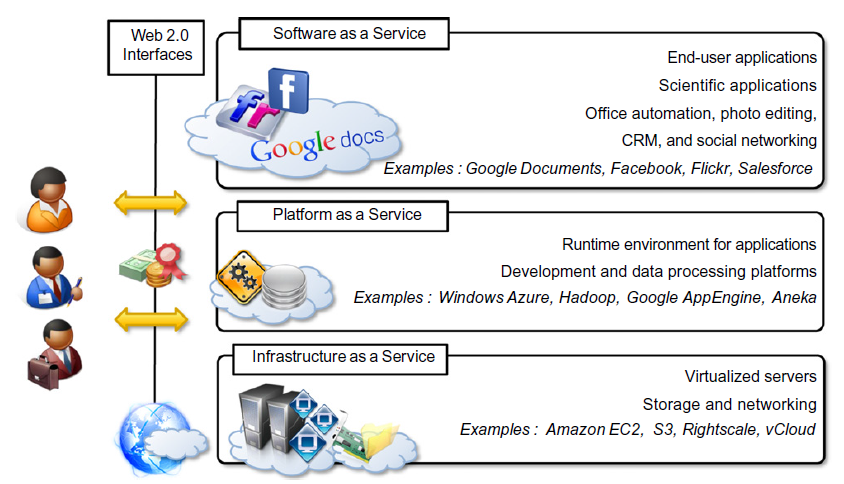
\includegraphics[scale=0.4]{service_models}}
\caption{Cloud Service Models \cite{masteringcloudcomputing}.}
\end{figure}

\textbf{Infrastructure as a Service} is the offering of virtualised resources (computation, storage, and communication) on demand\cite{vimprivatehybrid}, allowing users to provision servers on demand, running different Operating Systems and even customised software stacks. IaaS offers the advantage of control over remote resources, which is often a good fit for a company with an established IT setup looking to benefit from the cloud. It also gives the option of working with highly customised or niche software which may not be offered as a service in itself. An example of IaaS is Amazon Web Services EC2, which offers Virtual Machines with software stacks that can be customised. \cite{principlesparadigms}\\ \\
\textbf{Platform as a Service} offers a higher level of abstraction than IaaS, providing a platform which is more easily programmable. PaaS delivers scalable and elastic runtime environments on demand and host the execution of applications\cite{masteringcloudcomputing}. The cloud provider often controls scalability and manages other issues such as fault tolerance, so users can focus simply on the logic of the application utilising the cloud provider's APIs and libraries\cite{masteringcloudcomputing}. One big advantage of this approach is the lack of concern about how the cloud actually works in terms of hosting the application; instead, the user is just guaranteed a stable, scalable environment for their application to run in. Google App Engine is a great example of PaaS, allowing deployment and hosting of Web Applications\cite{googleappengine}.\\ \\
Finally, the service with the highest level of abstraction is \textbf{Software as a Service}, which as a solution provides applications and services on demand\cite{masteringcloudcomputing}, such as the common elements of desktop applications like Office Suites or photo editing. Usually these applications are accessible through a browser, and will host files and configuration data in the cloud, making for an easy access, scalable alternative to a native desktop application. Google Docs is a very popular example of SaaS, allowing editing of spreadsheets, word documents, and more, which are then stored on its sister storage service, Google Drive\cite{googledrive}.   
 
\subsection{History}
Cloud Computing has been many years in the making. Many technologies have contributed to its inception; A visualisation of these can be seen in the below figure. To understand how Cloud Computing came about, it is important to note the types of problems which were being solved, and the previous solutions that inspired this movement. 
 
\begin{figure}[ht]
\centering
\fbox{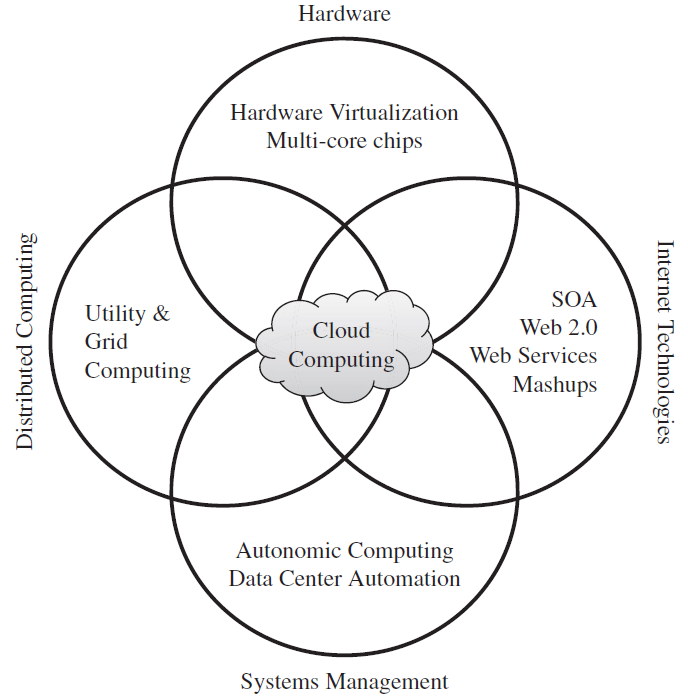
\includegraphics[scale=0.3]{roots_of_cloud_computing}}
\caption[An example figure.]{Convergence of advances leading to advent of Cloud Computing \cite{principlesparadigms}.}
\end{figure}

\textbf{Utility Computing}, i.e. the on demand delivery of infrastructure, applications, and business processes over the internet for a fee \cite{utilitybusinessmodel}, was the inspiration of a number of technologies over the years, as the idea brought great advantage to both utility providers and consumers. For providers, this meant lower operational costs, as infrastructure could be built to serve many different users, increasing efficiency and lower total cost of ownership \cite{utilityglobalgrids}. Furthermore, the economies of scale associated with building such an infrastructure allow providers such as Amazon to offer extremely low prices for their services \cite{amazonwhatiscloudcomputing}, a great benefit for consumers.  Other benefits for a consumer include the ability to adapt their usage rapidly to unpredictable needs, such as an online retailer which sees traffic spikes seasonally; more resources to handle this traffic can be acquired temporarily and released when the spike is over. Other huge advantages for company consumers are the lack of up-front infrastructure cost, and the speed and ease of deployment on the cloud \cite{amazonwhatiscloudcomputing}.    

The emergence of the \textbf{Web Service}, defined by W3C as: "\textit{A software system designed to support interoperable machine-to-machine interaction over a network}"\cite{w3cwebservice}, was a major factor in allowing the move from in-house computing power to utility-supported computing\cite{principlesparadigms}. Web Services contributed significantly to advances in software integration\cite{soapapazoglou}, gluing together applications on different platforms and hardware remotely, and allowing the free availability of information over the internet. It was this enabling of remote services that contributed to the realisation of utility computing and, eventually, the cloud. \\
Standardisation of Web Services on known technologies such as HTTP and XML made them ideal for \textbf{Service Oriented Architecture} (SOA), the purpose of which is to address the requirements of loosely coupled, distributed systems and their need for standards\cite{principlesparadigms}. \\
\textbf{Grid Computing} was one of the first major steps to realising the utility dream. It utilised the aforementioned standardised web services as a base for creating a system which aggregated distributed resources and allowed transparent access to them\cite{principlesparadigms}. Grids allowed on-demand access to computing resources over the internet. However, it was difficult to ensure Quality of Service in grids\cite{buyyamarketorientedcomputing}. This was due to a lack of performance isolation, so if resources were oversubscribed, one grid user could affect the performance given to another. Impossibility of ensuring QoS and execution time made the grid unsuitable for many applications, particularly those which were time-critical\cite{virtualworkspaces}. Virtualisation has been identified as the perfect solution for problems which have frustrated grid users. Indeed, some research projects like Globus Virtual Workspaces have added a layer to grids for virtualising computation, storage and network resources\cite{virtualworkspaces}. \\
\textbf{Hardware Virtualisation} technology, which uses hypervisor technology to split hardware resources, has contributed to the cloud through allowing data-centres to service the differing needs of consumers. The idea of virtualisation of resources for improving sharing and utilisation of computers has been established for decades\cite{surveyvmresearch}. This has now been adopted by cloud technologies such as Amazon's Elastic Compute Cloud \cite{amazonec2}. Virtualisation will be discussed in more detail later in this section. 

\subsection{Desired Characteristics \& Challenges}
In order to evaluate any Cloud technology, it is important to ascertain the characteristics of a Cloud which are more desirable, and those which present challenges to the running of a particular Cloud. In this way, it is possible to target experiments which exhibit and analyse the desirable aspects of a Cloud in a particular implementation, e.g. OpenStack, and also to perform experiments which analyse how well the implementation deals with certain well known challenges for Clouds. Some of these will require quantitative analysis, and some qualitative. 

A white paper released by Dialogic Inc.\cite{dialogiccloud} and Buyya et al.\cite{masteringcloudcomputing}\cite{principlesparadigms} identified a number of key beneficial characteristics of a Cloud. These included:

\begin{itemize}
\itemsep0em
\item Cost Savings - Reduced expenditure for increasing computing capability. Represents low barrier to entry to acquiring IT resources. 
\item Scalability / Flexibility - Growing resources and scaling back rapidly, using extra at peak times and less at off-peak. 
\item Reliability - Services using some means to support business continuity and disaster recovery. 
\item Accessibility - The ability to access a cloud in a number of ways, e.g. from a mobile as well as a standard browser. Clouds should also be available On-Demand in a Self-Service manner. 
\item Simplified application acceleration and scalability - Allowing for hosted applications to gain resources and scale up with minimal effort.
\item Energy Efficiency - Low power usage and lesser carbon footprint.
\item Efficient Resource Allocation - Lack of fragmented resources, virtual resources are allocated such that they increase performance or efficiency. 
\item Seamless creation and use of third party services - Allowing the composition of services to give flexibility of development, adding value to consumer products.
\item Elasticity - The illusion of infinite resources for a consumer. 
\item Customisation - Ability to customise resources given to consumers, by allowing root access for example.
\end{itemize}

These characteristics often represent advantages for both cloud providers and consumers, and so are usually important regardless of which service and deployment model are being used. \\ 

Cloud Computing does come with a number of challenges. Those identified by Dialogic \& Buyya et al. include:

\begin{itemize}
\itemsep0em
\item Security \& Privacy - Storing and transmitting sensitive data causes huge concern. This is especially a problem as data must be decrypted to be processed in the cloud, a 'weak point' in the chain. Often, security issues slow down deployment of cloud services. 
\item Lack of Standards - Clouds have documented interfaces; no standards are associated with these, so few clouds are interoperable. 
\item Continuous Evolution - User requirements evolve for interfaces, networking, storage, many different areas. Clouds do not remain static. 
\item Compliance Concerns - Data protection directives from the EU for example could affect cloud computing, based on what data being used. These laws can 'get in the way'. 
Technical/Practical problems - Such as with configuration, networking and sizing of complex systems. Size and scalability inherently bring such challenges. 
\item Dynamic Provisioning - Deciding on how best to provision resources, how many to provision and how long to use them for, attempting to optimise benefits from clouds.  
\end{itemize}

These are just a small number of the issues and challenges related to Clouds, and again, often cause problems regardless of cloud configurations and architectural choices. It is for this reason that products like OpenStack must address these challenges. How effectively this is achieved will be part of this evaluation.


\section{Virtualisation}
\subsection{Introduction}
Virtualisation was defined by Amit Singh \cite{virtintro} as: "\textit{a framework or methodology of dividing the resources of a computer into multiple execution environments, by applying one or more concepts
or technologies such as hardware and software partitioning, time-sharing, partial or complete machine simulation, emulation, quality of service, and many others}." \\ \\
Virtualisation provides a number of capabilities which suit the needs of Cloud providers perfectly, including hardware-independence of OS and applications, capability of provisioning a 'Virtual Machine (VM)' on any system, and single unit management of multiple OS and applications through their use as 'VM's\cite{vmwareoverview}.  \\
The main advantage of this to an IaaS cloud however, is the split created between hardware and software resources, providing flexibility to provision and allocate resources in a very dynamic manner. The below figure illustrates how this split allows a multi-purpose system to be devised from a pool of hardware using a virtual infrastructure. 

\begin{figure}[ht]
\centering
\fbox{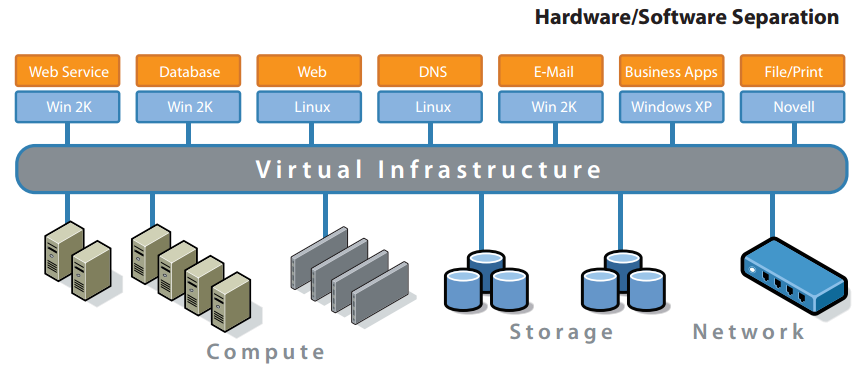
\includegraphics[scale=0.4]{hardware_separation}}
\caption{Virtual Infrastructure \cite{vmwareoverview}.}
\end{figure}

As has been previously established, Virtualisation technology is not only commonly in use in current cloud technology, but was also one of the chief driving factors contributing to the advent of Cloud Computing. Virtualisation is extremely important for products such as OpenStack due to their use as an IaaS provider. This, particularly in public cloud deployments, often means very large pools of hardware resources, such as data centres, needing the flexibility and elasticity a cloud should provide; virtualisation is key to achieving this goal. 

%\subsection{Types of Virtualisation}

\subsection{The Data Centre}
Cloud computing services are usually backed by large-scale data centers composed of thousands of computers. Such data centers are built to serve many users and host many disparate applications. For this purpose, hardware
virtualization can be considered as a perfect fit to overcome most operational
issues of data center building and maintenance\cite{principlesparadigms}. 

\begin{figure}[ht]
\centering
\fbox{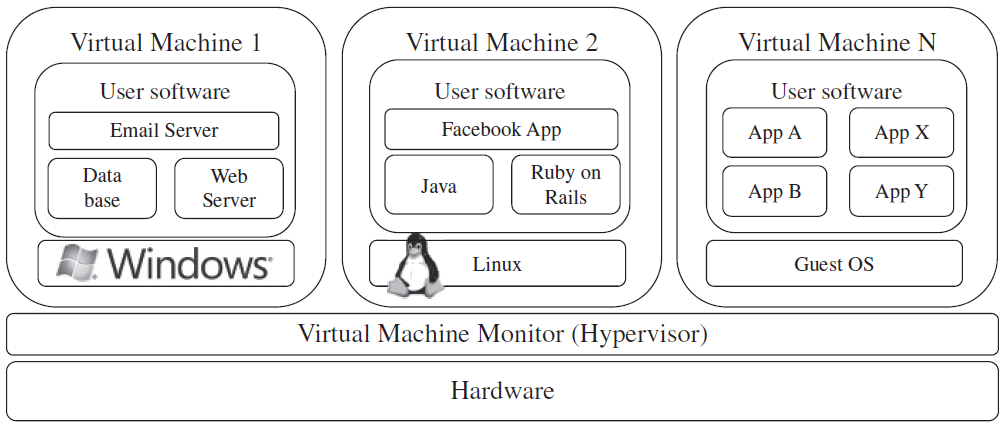
\includegraphics[scale=0.35]{vmhypervisor}}
\caption{Hardware Virtualised server hosting \cite{principlesparadigms}}
\end{figure}

This move towards the data centre has happened for a number of reasons. The first, and most obvious reason, is that use of large pools of hardware effectively utilises the capabilities of virtualisation; this power of splitting hardware in a number of ways is less effective, and often unnecessary on smaller sets of hardware.  \\
Cost Efficiency has been a huge driving factor in the trend towards the data centre and virtualisation; Virtualisation has been proven to reduce both capital expenditures (e.g. servers, storage) and operating expenses (e.g. maintenance 
 fees, management costs)\cite{agilysis}. Another enormous factor is improved server utilisation. Many data centers have servers that use anywhere from 
 5\% to 15\% of their actual capacity, with the rest going unutilized\cite{agilysis}. Due to the ability to migrate VMs and reallocate resources from certain servers to others, this figure could be greatly improved by using virtualisation, and this in turn would save money and time on power and wasted effort. \\ 
One enormous advantage of use of virtualisation, which is particularly relevant to OpenStack and this project, is the use of \textbf{Data Centre Infrastructure Management} (DCIM) solutions. Uptake of DCIM has been very high in recent years, with one analyst at Gartner stating "By 2017, DCIM tools will be significantly deployed in over 60 percent of larger data centers (over 3,000 sq ft) in North America."\cite{dcimautomation}. \\ 

DCIM is a general term for solutions aimed at improving management and automation of a data centre in terms of it's resources; those which are interesting to a cloud provider using virtualisation are \textbf{Virtual Infrastructure Managers}. These will be discussed in detail in the next part of this section. 
   
\subsection{Virtual Infrastructure Management}
Virtual Infrastructure Managers (VIMs) are software toolkits responsible for the orchestration of resources so as to rapidly and dynamically provision resources to applications\cite{vimprivatehybrid}. This type of software often resembles a traditional Operating System (OS), but instead of dealing with a single computer, it aggregates resources from multiple computers, presenting a uniform view to users and applications\cite{principlesparadigms}. Often, they are referred to as a \textbf{Cloud OS}\cite{vmwarevsphere}. \\ 
The aim of a VIM is to\cite{vimprivatehybrid}:
\begin{itemize}
\itemsep0em
\item Provide a uniform, homogeneous view of virtual resources, regardless of underlying platform. 
\item Manage the full lifecycle of a VM, including tasks like provisioning VM networks and storage. 
\item Support configurable resource allocation policies e.g. high availability, server consolidation. 
\item Adapt to the changing resource needs of an organisation. 
\end{itemize} 

\subsection{Features of VIMs}
A great number of VIMs investigated by Buyya et al.\cite{principlesparadigms} present a set of basic features related to managing VMs. These features all but define whether a tool can be used for cloud deployment. However, only a small number of those investigated exhibit features such as high availability, which allow them to be used in large-scale production clouds. These features, taken from their investigation, include:

\begin{itemize}
\itemsep0em
\item \textbf{Virtualisation Support} - Multi-tenancy in clouds requires multiple customers with disparate requirements to be serviced by the same hardware pool. Virtual resources can be resized easily with flexibility. This makes virtualisation the best option for a data centre servicing multiple tenants, as is the case with a cloud.  
\item \textbf{Self-service, On-Demand Resource Provisioning} - One of the most attractive features to a cloud. Enables users to directly obtain services from clouds, without interacting with a sysadmin. This "\textit{Eliminates the need for more time-consuming, labor-intensive, human driven procurement processes familiar to many in IT}"\cite{webspherejournal}.
\item \textbf{Multiple Backend Hypervisors} - Different virtualisation models and tools have different benefits and drawbacks. Due to this, some products offer a uniform management layer that is capable of sitting on top of many different hypervisors; in this way, a business may choose that which is right for them, or even switch without a change in how they manage their infrastructure.  
\item \textbf{Storage Virtualisation} - This means abstracting logical storage away from physical storage. By consolidating all storage in a data centre, a user can create virtual disks independent of any storage device or location. Often these are organised in a Storage Area Netwoek (SAN) and are attached to servers using protocols like Fibre Channel, iSCSI, and NFS. A storage controller provides the layer of abstraction between virtual and physical storage\cite{serverstoragevirtsingh}. Virtualisation of storage is usually more common in commercial products such as VMWare, and others just provide ways of managing storage devices. 
\item \textbf{Interface to public clouds} - Use of Cloud-bursting to extend the capacity of local in-house infrastructure is common, and if a VIM can automate or at least facilitate the 'borrowing' of capacity from a public cloud, this would be very advantageous. In this way, a VIM can support operation of a Hybrid Cloud. 
\item \textbf{Virtual Networking} - Virtual Networks allow creating an isolated network on top of physical network infrastructure independent of physical topology and locations\cite{interconnections}. A virtual LAN (VLAN) allows isolating traffic, allowing VMs to be grouped in the same networks. Most VIMs offer virtual networking capability. Some even support use of Virtual Private Networks (VPNs) for contacting local and remote VMs when using Cloud Bursting. 
\item \textbf{Dynamic Resource Allocation} - Capacity management and demand prediction are complicated in systems servicing variable and dynamic need. These problems along with awareness of energy consumption have lead to the need for dynamic resource allocation aiming at obtaining a timely match of supply and demand \cite{capacitymanagement}. Dynamically remapping VMs to physical machines at regular intervals can reduce energy consumption and better service dynamic demand. Many VIMs support features which monitor utilisation across resource pools and reallocate available resources among VMs according to application needs. 
\item \textbf{Virtual Clusters} - Some VIMs can holostically manage groups of VMs. This is useful for provisioning computing Virtual Clusters on Demand, and interconnected VMs for multi-tier Internet Applications\cite{oneclickvirtualclusters}.
\item \textbf{Reservation System} - These are systems which allow users of an infrastructure to request resources. When users request computational resources at a specific time, requests are termed advance reservations (AR). Best-effort requests are those where users request resources whenever available\cite{batchexecutionleasing} Leases on resources can be negotiated, allowing an agreement between consumer and provider. This goes a way towards allowing different users to consume the same infrastructure in a structured manner, without too much stepping on toes. 
\item \textbf{High Availability \& Data Recovery} - High Availability in VIMs aims at minimising application downtime and preventing business disruption. A few VI managers accomplish this by providing failover mechanisms, which detect both physical and virtual failures and restart VMs on healthy servers. This style of HA protects from Host, but not VM failures \cite{vmwarehighav}\cite{citrixhighav}. Sometimes, for example in critical systems, this type of failover is not enough. In this case, additional levels of fault tolerance relying on redundancy of VMs are implemented. A system will monitor when a VM or system component fails and ensures that a duplicate VM serves any application in case of failures \cite{citrixhighav}.     
\end{itemize}
Targeting experiments to exhibit these features will be a useful way to assess the capabilities of OpenStack versus its competitors. 

\subsection{Current VIM Technologies}
In order to gain some context as to the involvement of OpenStack in the Cloud Computing industry, it is important to gain some insight as to its competitors and similar products. This should also provide a good point of comparison for the evaluation of OpenStack. 
The technologies I have chosen to introduce are three of the largest and most popular current implementations. These are Eucalyptus, OpenNebula and Nimbus. A feature comparison of these three technologies can be seen in the figure below. 

\begin{figure}[ht]
\centering
\fbox{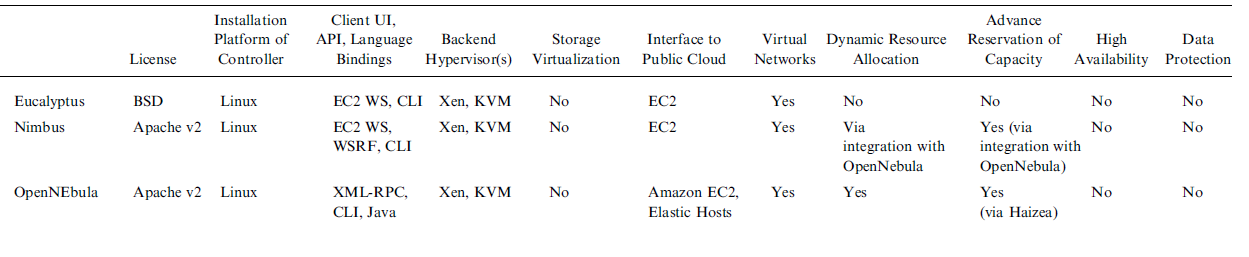
\includegraphics[scale=0.5]{VIM_comparison}}
\caption{Feature comparison of Virtual Infrastructure Managers \cite{principlesparadigms}.}
\end{figure}

\textbf{Eucalyptus}\\
Eucalpytus\cite{eucopensourcesystem} is a free, open-source tool for building Amazon Web Services (AWS) compatible private and hybrid cloud environments. It was one of the first of its kind to focus on the development of Infrastructure as a Service clouds. 
The idea behind the project was to develop an open-source implementation which would provide identical functionality and APIs to the AWS implementation, meaning that tools developed for AWS EC2, one of the most popular proprietary IaaS cloud frameworks, would also be compatible with Eucalyptus. Eucalyptus was a relatively early project, having started in 2008, but with a project called the Virtual Grid Application Development Software project, started in 2003, being one of it's main influences\cite{eucopensourcecloudsystem}.   \\ 
The project's features are split into different sections based on functionality; these, along with AWS compatibility, are Compute, Networking, Storage, Self-Service Provisioning and Cloud Management\cite{eucalyptusfeatures}. Notable features within these sections include\cite{eucalyptusfeatures}:

\begin{itemize}
\itemsep0em
\item Support for Leading Hypervisors - support for leading hypervisors such as KVM and VMware vSphere.
\item Auto Scaling - scale Eucalyptus resources up or down based on policies defined using EC2-compatible APIs and tools. 
\item CloudWatch - Provides a reliable and flexible monitoring solution for cloud resources and applications running in Eucalyptus. 
\item Elastic Load Balancing - Distributes incoming application traffic across multiple Eucalyptus instances, providing greater fault tolerance for applications.
\item Snapshot Management - snapshot and protect data stored in block storage volumes
\item Instance Management - create, manage, and delete instances.
\item Web-based Administrator Console - Performs cloud management functions such as viewing cloud resources and logs and managing virtual machine images.
\item Zero Downtime Cloud Maintenance - Leverages hypervisor live migration technologies to enable zero downtime maintenance on hardware nodes for greater application uptime.
\end{itemize}

\textbf{OpenNebula}\\
The OpenNebula project, started as a research project in 2005 by Ignacio M. Llorente and Rubén S. Montero, aims to provide efficient and scalable management of virtual machines on large-scale distributed infrastructures\cite{opennebulaaboutproject}. Due to its age, since it's first release in 2008, OpenNebula has become a mature product which solves many business needs for companies needing data centre VM management. These features allow it to be used to build public, private or hybrid IaaS clouds\cite{opennebulaabouttech}. OpenNebula is free and Open Source, under the Apache License v2, and has an active community of developers and users, with several thousand downloads per month \cite{opennebulaaboutproject}. OpenNebula appears to be a very well designed project, with objectives and design principles set in place which lead to a very clearly defined vision for the project\cite{opennebulaabouttech}.\\
Some of the key features of OpenNebula include\cite{opennebulafeatures}: 

\begin{itemize}
\itemsep0em
\item AWS EC2 and EBS APIs.
\item On-demand provision of Virtual Data Centers.
\item Automatic installation and configuration of application environments 
\item Powerful CLI that resembles typical UNIX commands applications.
\item OpenNebula Marketplace is a catalog of virtual appliances ready to run in OpenNebula environments
\item Powerful and flexible Scheduler for the definition of workload 
\item High availability architecture.
\item Cost-effective failover solution.
\end{itemize}

Interestingly, CERN, one of the largest and most advanced physics labs in the world, has recently replaced its OpenNebula environment with one using OpenStack, mainly due to the ecosystem of OpenStack being more desirable, and a number of scenario tests of OpenNebula under various conditions\cite{cernopennebula}.  

\textbf{Nimbus}\\
Nimbus is a free, open source toolkit that, once installed on a cluster, allows the provision of an IaaS cloud via Web Services. The application is aimed chiefly at the scientific community\cite{nimbusabout}. The project is based on three main goals; firstly, to enable providers of resources to build private or community IaaS clouds. Secondly, to enable users to use IaaS clouds, and thirdly, to enable developers to extend, experiment and customize IaaS\cite{nimbusabout}. This approach of considering use cases is an interesting topic of evaluation, and could be useful for this evaluation of OpenStack. \\
Notable features of Nimbus include \cite{nimbusfeatures}:
 
\begin{itemize}
\itemsep0em
\item Remote deployment and lifecycle management of VMs
\item Compatibility with Amazon's Network Protocols for EC2 and S3.
\item Easy to Use Cloud Client.
\item Per client usage tracking, per user storage quota. 
\item Configuration management at deploy time. 
\item One-click clusters - auto-configuration of entire clusters.
\item Workspace client - allows authorized clients to access all Workspace Service features. 
\item Xen and KVM plugins. 

\end{itemize}

\section{OpenStack}
\subsection{Introduction}
OpenStack is "\textit{a global collaboration of developers and cloud computing technologists producing the ubiquitous open source cloud computing platform for public and private clouds}"\cite{openstackhomepage}. The project aims to "\textit{deliver solutions for all types of clouds by being simple to implement, massively scalable, and feature rich}\cite{openstackhomepage}". The technology consists of a number of different interrelated projects all delivering various components which allow creation of cloud infrastructure. \\ 
OpenStack was founded by Rackspace Hosting and NASA, and was first publicly released in 2010. Since then, under the OpenStack foundation, the OpenStack community has grown immensely, with over 10,000 technology professionals in 133 countries having involvement in the project. Aside from the community, popularity of the product has increased greatly since its inception, and it is currently used by corporations, service providers, VARS, SMBs, researchers, and global data centers looking to deploy large-scale cloud deployments across the world. One important aspect of the product is that it is Open Source under the Apache 2.0 license, meaning that anyone can use or contribute to the project.  
Since the inception of the OpenStack foundation in 2012, more than 200 companies have joined the project, including Arista Networks, AT\&T, AMD, Brocade Communications Systems, Canonical, Cisco, Dell, EMC, Ericsson, F5 Networks, Groupe Bull, Hewlett-Packard, IBM, Inktank, Intel, NEC, NetApp, Nexenta, Rackspace Hosting, Red Hat, SUSE Linux, VMware, Oracle and Yahoo!\cite{openstackcompanies}. Many of these companies are also clients of the software. 

\subsection{Overview of Technology}
\subsubsection{Aims of the Project}
OpenStack's mission is "\textit{to enable any organization to create and offer cloud computing services running on standard hardware}" \cite{openstackhomepage}. This is a broad aim, and is the basis of the entire project. 
The long term goal of the project, taken from OpenStack's FAQ section, is "\textit{to produce the ubiquitous Open Source cloud computing platform that will meet the needs of public and private cloud providers regardless of size, by being simple to implement and massively scalable.}"\cite{openstackfaq}. Already it is clear to see that OpenStack's aims are in line with many desired cloud characteristics, such as scalability and simplicity. 
The project is targeted for use by "\textit{service providers, enterprises, government agencies and academic institutions that want to build public or private clouds. Industries range from IT \& telco to SaaS and eCommerce to finance and healthcare.}" \cite{openstackfaq}. Clearly this project is aimed at large scale, often enterprise providers, and so it will need to have high reliability and a range of capability. 
There seems to be an emphasis on the project being very open to the community. When asked 'If there are other open source cloud projects, why create a new one?' the foundation responded: "\textit{We wanted a community where people with similar philosophies about cloud architecture and open-source software can openly collaborate together. We believe in open source, open design, open development and an open community that is fully transparent? Not a cathedral, a bazaar.}"\cite{openstackfaq}
Overall, it seems that the objectives of the project are similar to those of previously created similar products, such as Eucalyptus. In this sense, OpenStack becomes a spiritual successor to these products, being the newer product, growing in popularity. 

\subsubsection{Design/Architecture of Project}
\begin{figure}[ht]
\centering
\fbox{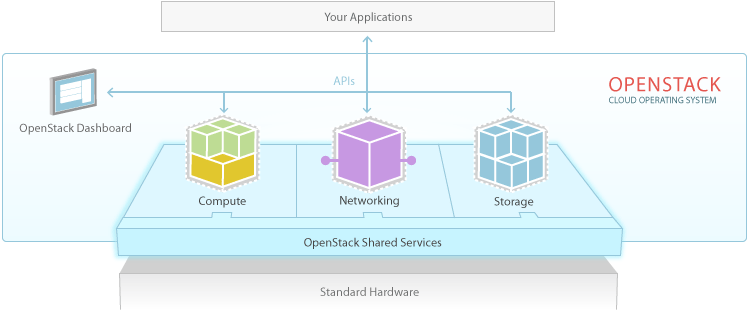
\includegraphics[scale=0.4]{openstack-software-diagram}}
\caption{Overview of OpenStack architecture \cite{openstacksoftware}.}
\end{figure}

OpenStack the project consists of a number of interrelated components, all of which work together to provide Cloud Infrastructure. These projects include\cite{openstacksoftware}:

\begin{itemize}

\item \textbf{Compute (Nova)} - Provisions and manages large networks of virtual machines.
\item \textbf{Object Storage (Swift)} - A cost effective, scale-out storage platform. 
\item \textbf{Block Storage (Cinder)} - Allows block devices to be exposed and connected to servers
\item\textbf{ Networking (Neutron)} - A Pluggable, scalable, API-driven network and IP management.
\item \textbf{Dashboard (Horizon)} - A web based Graphical User Interface for use of OpenStack.
\item \textbf{Identity Service (Keystone)} - A common authentication system across the OpenStack cloud operating system. 
\item\textbf{ Image Service (Glance)} -  Provides discovery, registration and delivery services for disk and server images. 
\item \textbf{Telemetry (Ceilometer)} -  Aggregates usage and performance data across OpenStack
\item \textbf{Orchestration (Heat)} - template-driven engine to automate the deployment of infrastructure.
\end{itemize}

\section{Current Evaluations of OpenStack}
Reading current evaluations of OpenStack gives a good idea of the types of approach and criteria used by other researchers or organisations to evaluate a product like OpenStack. Of those which were part of this literature review, a brief description of their approach and conclusions will be provided, with the hope that some inspiration can be taken for this evaluation. 

One evaluation, performed by the Engineering Task Force (ETF)\cite{etfevaluation}, gave a brief evaluation of OpenStack as part of a range of Cloud Software evaluations.
This evaluation appears to have very modest aims; simply to provide an overview of the OpenStack technology, similar to the 'Technology Overview' in this section. A brief history of the project and an overview of its components is provided in the first part of the paper. 
Another huge part of this evaluation focuses on deployment of OpenStack from the perspective of the Server and the Client; instructions of how to get a basic configuration set up are given, and a break down of some basic tasks that can be performed, such as user management, are provided. 
Finally, there is a focus on User Experience, something which is of clear importance to the ETF. This considers what the user must do to perform certain tasks involved with management and maintenance of a deployment. A short conclusion is provided, which refers to OpenStack as a "\textit{mature, well-backed software for
implementing an Infrastructure as a Service Cloud}\cite{etfevaluation}".\\
It appears that this evaluation focuses on the deployment of OpenStack and on its basic usability; it may then be a good idea to take this a step further, but with a similar approach. It has elements of both Quantitative and Qualitative evaluation, which seems a good approach. \\

A second evaluation that was covered as part of this literature review was the plan published by CERN for their own evaluation\cite{cernevaluation}. The results were not available, but the plan itself gives a very good indication of the approach taken by CERN in their evaluation, and this is clearly most important when considering how to approach another evaluation. This process appeared to be a little more developed than that of the ETF, and had a clear schedule of which tasks would be performed and evaluated. Steps included setup of hypervisors, launching of basic images, validation of dynamic shrinking and growing of resources, etc. It appears that the idea behind this particular evaluation was to analyse OpenStack by simply using it, and deliver a deployed OpenStack solution, similar to the initial aims of this evaluation. Again, a mix between qualitative research and quantitative practical work seem to be the desired approach, and one which this evaluation will likely follow. \\

From considering these two evaluations, it appears that there is a lot of room for new experimentation with OpenStack, particularly with respect to its integrated functionality and shared services. The approaches in these two, particularly CERN's approach, give a great starting point and list of tasks which have been identified as important to evaluate. These evaluations, and indeed any others that could be found, do not go into great detail, or give any comparison with other technologies, and so this is an untapped area which may provide some value, particularly for projects and organisations choosing between several solutions in future.  

\section{Plan for Evaluation of OpenStack}
\textbf{What is 'Evaluation'?}\\
When deciding to 'evaluate' OpenStack, it must be clear what is actually meant by the term 'evaluation'; the word is very vague, and evaluations can take many different forms. In order to decide, the aims \& justifications of the project must be considered:

\begin{itemize}
\itemsep0em
\item Provide knowledge of OpenStack (for the ASCETIC Project).
\item Provide some validation of OpenStack (for the ASCETIC Project).
\item Investigate the popularity of OpenStack.
\item Assess the validity of OpenStack based on its features \& capabilities.
\end{itemize}

From this, 5 main possible definitions of 'Evaluation' were drawn:

\begin{itemize}
\itemsep0em
\item Written guides of how to use OpenStack.
		\textit{This form of evaluation was used by the ETF, and was actually used for a similar purpose; as a precursor to a larger project.}
\item Functionality validation of OpenStack - i.e. validating first hand it actually does what it claims.
\textit{This was employed by CERN in their evaluation. It also was used to prepare an OpenStack deployment for another project.}
\item A review of OpenStack functionality.
\textit{Would tie in to the first two evaluations, gives an indication of how good OpenStack is based on various metrics.}
\item A comparison of OpenStack with similar competitors such as OpenNebula.
\textit{This was used by the ETF, but will be difficult in this project due to lack of resources.}
\item  A quantitative analysis of the capability of OpenStack - i.e. how well it performs certain actions.
\textit{This was not used excessively by either evaluation, but may be useful to bring new value to the domain.}
\end{itemize}

\textbf{Evaluation Considerations}\\
It is important after establishing context and analysing previous evaluations through literature review to establish some ideas concerning this evaluation of OpenStack. These can be established through a number of sources, including, but not limited to:

\begin{itemize}
\itemsep0em
\item The Aims \& Objectives of the Project - to provide some evaluation of OpenStack functionality, along with some comparison with competitors. 
\item The project deliverables - an evaluation report with designed experiments to test OpenStack, re-usable software components for use of OpenStack. 
\item The literature review - Particularly past evaluation approaches, and such useful information as desired aspects of a cloud. 
\end{itemize}

It would be extremely difficult to perform a full and advanced evaluation of all of the features of OpenStack, as it is an enormous piece of software with hundreds of use cases and features. This is where information such as the above comes in handy; it is possible to narrow the scope of this project so as to provide a fully contained and coherent evaluation, but one which does not require too much to be done than is possible in the time frame. \\

Firstly, from the recommendation of the CERN approach, the project will focus in part on use of OpenStack; experiments will be targeted at specific areas of functionality which are important, and that can be executed and demonstrated. Information from the literature review is very helpful in deciding which functionality is deemed important, as in this review, we have several guidelines on what aspects of a Cloud are important e.g. elasticity, but also those which are important to a Virtual Infrastructure Manager, e.g. multiple backend hypervisors. We even have a short overview of competitor products which should aid in qualitative feature assessment, and choice of important functionality. \\

Secondly, both of the reviewed evaluations attempt to mix qualitative and quantitative assessment, and this is something which will certainly be employed in this project; each style of assessment gives a very different view and perspective, and each can be seen as equally important, and indeed complementary when analysing software. It would of course be much easier to compare OpenStack to other implementations using qualitative assessment, as multiple deployments of different Cloud solutions is beyond the scope of this project, and so it would be difficult to obtain quantitative results to compare. \\

Finally, there are some areas in which I believe the current evaluations fall short. For a start, they do not contain any practical programmatic evaluation, and seem very focussed on systems administration. This is something which this project will attempt to include, and hopefully bring new value to this area. Furthermore, there does not appear to be much sophistication in the experiments given in previous evaluations, and this is also something which this project will attempt to tackle. Perhaps the use of programmatic automation will facilitate the ability to go into more depth when considering what functionality to assess, as it is much more difficult to manually run complex functionality from a Systems Admin's perspective. This project will aim to combine some dashboard UI experiments with automated tests, and qualitative assessment. 

\section{Conclusion}

This section has aimed to introduce \& describe the various concepts and technologies which need to be understood for this project. It has laid out concepts, referenced literature, and used this to further define the problem at hand, and how to tackle it with this project. By now, the reader should have some understanding not only of the reasons and approach of the project, but also what kind of technical work it will require, and the impact it will have on the domain. This section has aimed to provide 'context' to the project, and give it some basis in the real world. It has also aimed to further define the problem at hand, in this case an 'Evaluation' by considering previous evaluations of OpenStack, and other relevant information.  \\
In the next section, the work described in Chapters 1 \& 2 will be laid out, executed and delivered. The results of each piece of work will also be discussed. Following the next chapter, these results, and the project as a whole, will be evaluated based on a number of factors described in Chapter 4.    

\chapter{Design \& Implementation}
\label{CHAP_THIRD}
\centerline{\rule{149mm}{.02in}}
\vspace{2cm}
This section of the report corresponds to the 'Implementation Phase' of the project plan. In this section, experiments will be designed, implemented, tested and executed, with results analysed. This will then be evaluated in Chapter 4: Evaluation. 
\section{Warm-up Exercises}
To allow for effective experimentation with OpenStack, a number of warm-up exercises were performed to allow for configuration of resources, choosing of technologies, and general learning around the use of the involved technology. 
These warm up exercises ranged from Systems Admin work, Development, and basic investigation through research Using technologies. 

\subsection{Deploying OpenStack on the Test Bed}

Before any work on OpenStack could begin, an installed and configured instance was required to be accessible. For this, the University of Leeds School of Computing TestBed was used. The TestBed is a cluster of machines dedicated to facilitating research into Cloud Computing.\\
This was decided for a number of reasons; firstly, the EU project, ASCETiC, of which this project is a precursor of, requires the delivery of a locally installed and configured instance of OpenStack. Secondly, having a local installation allows for a more controlled environment, where certain factors such as hardware usage and network traffic can be more easily managed and monitored. One disadvantage of this is that the 'Cloud' is relatively small, with only a handful of allocated machines, and offers little resource scalability. For this, a public cloud such as Amazon EC2 would likely be required. \\
The below figure demonstrates the working of the SoC TestBed, with its use of a Virtual Infrastructure Manager:

\begin{figure}[H]
\centering
\fbox{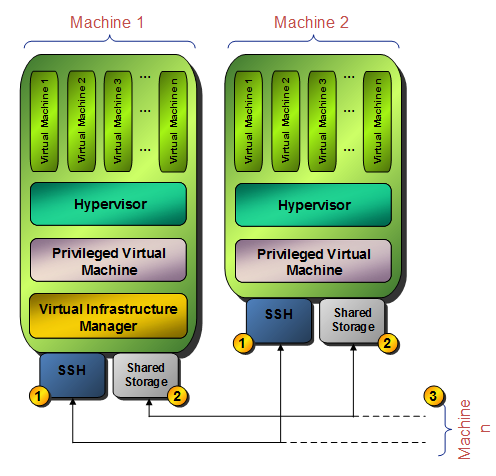
\includegraphics[scale=0.3]{cloudtestbed}}
\caption{Overview of the TestBed virtualised setup}
\end{figure}  

The current TestBed, consisting of 8 machines, uses OpenNebula, a competitor to OpenStack covered in the literature review of this report. However, in this project 2 machines have been allocated to this project and will use OpenStack to manage their resources as virtual infrastructure. 
Credit to Django Armstrong, who deployed OpenStack on the two machines in the Cloud TestBed for my use on this project, as I did not have the time or access privilege. 
These machines were accessed through the School of Computing network, using the machines Testgrid12 \& Testgrid13. The different projects such as Nova, Dashboard were available on different ports of this machine; e.g. port 443 for dashboard, \& port 5000 for Nova. This is in line with the general standard ports used in OpenStack\cite{openstackports}.  

\subsection{Experimenting with OpenStack - Experiment 0}
In order to learn how to interact effectively with OpenStack, I designed a first basic experiment which would require some interaction with at least 2 of its components. This experiment, as well as teaching me about OpenStack in general, would serve as a proof of concept for all future experiments, and provide examples of how to interact with OpenStack in 3 different ways, all of which may be used in future experiments; these are it's Web UI Dashboard, it's Command Line Interface, and it's Web Service APIs.\\
The experiment itself involves first authenticating a session via the OpenStack identity service, something which will be a prerequisite for almost every experiment, and to then perform a basic action using OpenStack compute, in this case creating a new Virtual Machine (VM) instance and starting it. In OpenStack, an instance is created from a template, known as an 'image' which is some configured software. I will introduce the chosen interaction method, describe how the experiment implementation was achieved in each case, and how they differed in approach, ease of use, and capability.  \\ 
The warm-up exercise described here can be found in Appendix E, and includes the results of each experiment, with details of the development environment(s) configured for this and further experiments.  

\section{Experiment Planning}

In order to get a good mix of Quantitative \& Qualitative evaluation, and to provide some useful practical information mixed with good coverage of OpenStack, the work to be done was set out as follows: 

\begin{itemize}
\item \textbf{Part 1: Architecture \& Feature Analysis of OpenStack} - Qualitative, descriptive analysis of the product. Overview of the product's design goals, choices, and its architectural characteristics will be provided, and an overview of the features of each component will be covered and explained, whilst being compared with the desirable and undesirable aspects of a cloud or VIM. 

\item \textbf{Part 2: Exploring OpenStack through Experimentation} - In this section of the report, several 'Experiments' will target specific functionality in OpenStack, and will demonstrate it through the use of RESTful APIs, CLI or Dashboard. Descriptions of the involved features and a review of their use will be given as a guide to using this functionality, as well as conclusions about the effectiveness of OpenStack's implementation. 

\item \textbf{Part 2b: Developing an OpenStack REST Client} - As previously mentioned as an aim of this project, a Java-based re-usable REST API client will be developed, in order to provide value to OpenStack users, and to perform experiments in part 2. This will be described in a separate appendix (E).
\end{itemize}

\section{Part 1: Analysis of OpenStack}

In this section, it is important to keep in mind the background research section of this report, specifically the 'Desirable Characteristics \& Challenges' of clouds and the 'Features of VIMs' section. The analysis below attempts to match OpenStack functionality to these factors to prove qualitatively that OpenStack is a valid and viable Cloud/VIM solution.  It will then go on to describe the benefits \& drawbacks of OpenStack functionality and features. 

\subsection{Architecture \& Feature Analysis of OpenStack}

The functionality of OpenStack is split into a number of different components, each of which are shown in the below figure detailing its architecture. Each component will be outlined in this section, along with its various notable features, uses and capabilities. It will then be analysed in terms of a number of basic metrics, including \textbf{coupling} and \textbf{cohesion}, and conclusions will be drawn about architectural choices. 

It is important to have a good understanding of the OpenStack offering so as to understand why it is good at what it does, how it deals with scale, and various other factors which determine whether it should be used for creating a Cloud.

\subsubsection{At a Glance}
\textbf{Introduction: }
Applications sit on top of OpenStack, utilising the infrastructure it provides via its APIS. This infrastructure is composed of Compute, Networking and Storage, all combined through OpenStack Shared Services, and accessed and managed via the OpenStack Dashboard. This allows the 'Cloud OS' openstack to be layered over commodity or standard hardware. Components each have their own REST APIs. 

\begin{figure}[H]
\centering
\fbox{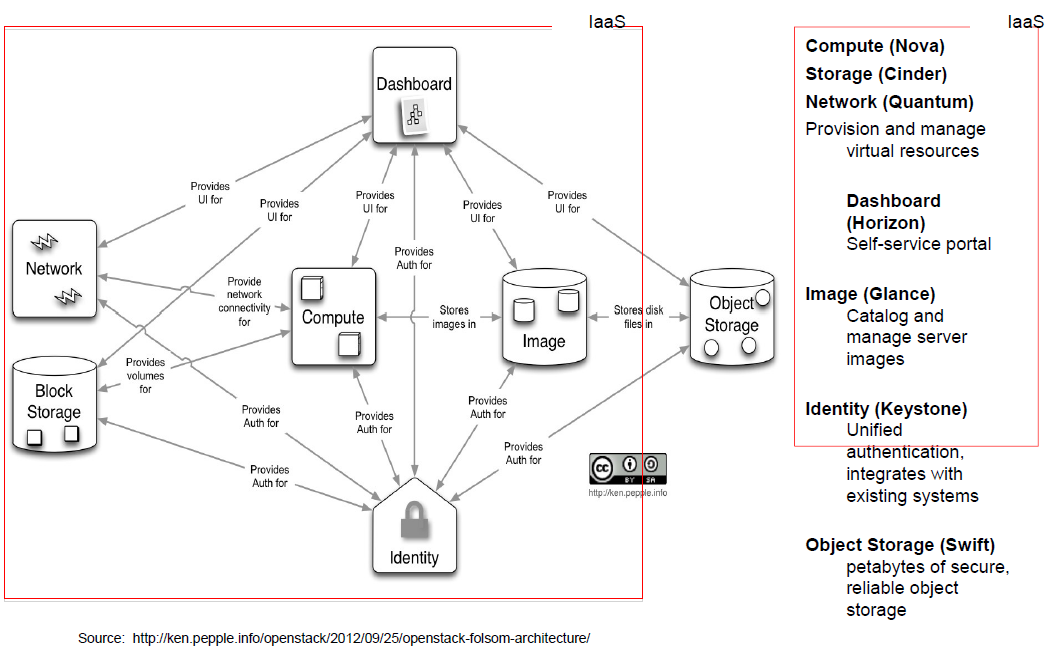
\includegraphics[scale=0.4]{openstack-architecture}}
\caption{Overview of OpenStack architecture \cite{openstacksoftware}.}
\end{figure}

\textbf{Analysis:}
The first noticeable feature of OpenStack's architecture is its number of distinct components, each of which interact with the others to provide Infrastructure as a Service. This is an interesting decision by the project designers, and differs greatly from similar projects such as OpenNebula. Conceptually, the design of OpenStack shows High Cohesion and Low Coupling. The functionality is split well into distinct blocks, each dedicated to a specific job, and handling, for the most part, only that job. The components communicate with each other through standards-compliant APIs in order to provide a fully functioning IaaS service. 

One considerable advantage of this approach, in line with the desirable aspects of a cloud discussed in chapter 2, is the level of customisation available to a consumer. Components can be left out, or even replaced with others, meaning that configurations of OpenStack are wide and varied, based on the needs of the users. In simple use cases, this can massively simplify the use and deployment of OpenStack, as only a small number of components need be configured, in turn saving on costs. Similarly, the approach effectively tackles one of the main challenges of the cloud - continuous evolution. When user requirements change, for example, more advanced networking is required, basic networking can be replaced with the neutron project. In this sense the 'cloud' need not be static. 
However, there may be some problems with this approach. Firstly, the level of complexity of communication is aptly displayed by the above figure; not only would this be difficult for professionals conceptually, but it could cause significant load, particularly on network performance, with so many distinct components constantly interacting. The issue of too much coupling and dependency in the system could also be a problem, if certain module dependencies are not fulfilled, such as Keystone for authenticating Nova requests. 

In terms of notable VIM features, OpenStack ticks many boxes. Virtual networking, storage, and dynamic resource allocation, and authentication are all provided by their own dedicated projects within OpenStack, meaning that, on paper, it really does satisfy most of the criteria for a working VIM. 

\subsubsection{Dashboard (Horizon)}

\textbf{Introduction:}
The OpenStack dashboard provides administrators and users a graphical interface to access, provision and automate cloud-based resources\cite{openstackdashboard}. It was designed in such a way that it can be combined with or used with third party services, such as those involved with billing, monitoring, or additional management. 

\textbf{Main Features:}
The dashboard is brandable, allowing users to make the tool available to its users in turn. The dashboard itself is a web application, and allows cloud administrators and users to control their compute, storage and networking resources. It also provides an overall view of the size and state of a cloud. Users and projects can be created, and users assigned to projects with set limits on the resources for those projects. Finally, and perhaps most notably, the dashboard offers users a self-service portal to provision their own resources within the limits set by administrators\cite{openstackdashboard}. This is one aspect of a cloud that we have established is very desirable. 

\textbf{Analysis:}
The first notable benefits of the Horizon project are its provision of a self-service portal for tenants in an IaaS cloud, which in turn allows the self-service provision of resources, one of the main desirable aspects of a cloud, and of a VIM. This is possible because the Dashboard allows simple interaction with the other OpenStack projects, such as Nova, which handles resource provision. 
Another key point aspect of clouds provided by Dashboard is accessibility; it can be securely accessed over a network connection, and so reliable accessibility is possible. 
By far the most distinctive aspect of the component is the gradual learning curve it provides. For me personally, many of the concepts regarding OpenStack were learned through using the Web UI, as it is informative, and extremely simple to use. This in turn gives users a much better grasp of OpenStack as a whole. 
 
The level of integration offered by Dashboard is unparalleled across the OpenStack offering, and it is in fact difficult to see which project is being used at times, due to the abstract nature of User Interfaces. This fact can be both a blessing and a curse; it is good for a user to focus on the task at hand, and not have to worry about disparate functionality, but it is also difficult to spot which components are used more than others, or even whether some are necessary. The level of information given on project components is good using Dashboard, and this goes some way to solving this issue. 
One problem I did spot when using Dashboard, and leading on from the abstraction mentioned, is that it uses naming often inconsistent with other parts of OpenStack. For example, 'instances' are managed using the Dashboard, where the equivalent Nova API calls would handle 'servers'. This is a subtle difference, but can be extremely confusing for users. 

\subsubsection{Compute (Nova)}

\textbf{Introduction:}
The Compute part of OpenStack allows a business or other user to offer on-demand computing resources, by provisioning and managing large networks of virtual machines. Compute resources are accessible via APIs for developers building cloud applications and via web interfaces for administrators and users\cite{openstackcompute}. It is designed to scale horizontally as new hardware is added. 
Both KVM and XenServer hypervisors are available to use with OpenStack, although other hypervisors are also available;  Linux container technology such as LXC is also supported for scenarios where users wish to minimize virtualization overhead and achieve greater efficiency and performance. In addition to different hypervisors, OpenStack supports ARM and alternative hardware architectures\cite{openstackcompute}. \\
Popular use cases of this component include offering IaaS compute further up the stack, processing big data with tools such as Hadoop, scaling compute to meet unpredictable demand, and HPC elements with diverse and intensive workloads. 

\textbf{Main Features:} 
Notable features of Compute include\cite{openstackcompute}:
\begin{itemize}
\itemsep0em
\item Management of virtualized server resources such as
CPU, memory, and network interfaces.
\item Manage Local Area Networks (LAN)
\item Virtual Machine (VM) image management, and live VM management.
\item Store and Manage files programmatically via API
\item VM Image Caching on compute nodes for faster provisioning of VMs.
\end{itemize}

\textbf{Analysis: }
Nova is the 'bread and butter' of OpenStack as a Virtual Infrastructure Manager. It provides a number of key cloud characteristics, such as virtualisation support, elasticity of resources, and effective resource allocation. 
The ability to access nova via the command line, REST APIs and the Dashboard means that it provides accessible, self-service resource provisioning for the full VM lifecycle.  
Flavors, a concept introduced in the warmup exercises, allow for servers to be built at different sizes, and even running servers can be rebuilt at different resource sizes, giving a great level of elasticity. The ability to launch new servers from either images, i.e. bootable files, and snapshots of servers hugely accelerates the use and simplicity of the Nova functionality. Server migration offers efficient allocation of virtual resources, and Nova can even decide automatically the best server to migrate a server to. Aside from this, detailed information on resources is provided using Nova, meaning management of resources is very simple. 

Clearly, we can see that Nova provides all the functionality it takes to run an Infrastructure cloud. There were some problems I noticed, however, with the design of this component. As Nova is so important, it appears that concepts from other projects have been 'borrowed' so as to allow no dependence on other projects, such as the Glance Image service. This points to low cohesion, where the functionality of the Nova API can often seem out of place - it appears that nova tries to 'do it all' with concepts of images, networks, and flavors in it's API. Not only does this make for a badly designed API, but it can confuse users when trying to use Nova with other components, or even make other components redundant. 

\subsubsection{Networking (Neutron)}

\textbf{Introduction:}
OpenStack Networking is a pluggable, scalable and API-driven system for managing networks and IP addresses. It ensures the network will not be the bottleneck or limiting factor in a cloud deployment and gives users real self service, even over their network configurations\cite{openstacknetwork}.

\textbf{Main Features:}
The notable capabilities of Networking include\cite{openstacknetwork}: 
\begin{itemize}
\itemsep0em
\item flexible networking models e.g. flat networks or VLANs for separation of servers \& traffic.
\item manages IP addresses, allowing for dedicated static IPs or DHCP. 
\item Users can create their own networks, control traffic and connect servers to networks.
\item Administrators can take advantage of software-defined networking (SDN) technology.
\item extension framework allowing additional network services.
\end{itemize}

\textbf{Analysis: }
The feature list for the Neutron project is very impressive. The provision of Virtual networking is an essential for a VIM, and the ability to make use of the very important Software Defined Networking (SDN) technology shows that Neutron is very advanced in this area. Neutron provides a good level of customisation, allowing for flexible alternative networking models which make it ideal for adapting to changing user requirements. Users can self-serve using this functionality, and scale it down elastically with compute resources, making it a perfect partner for the Nova project. 

Neutron is a highly cohesive module; all functionality is dedicated to the management and maintenance of networking between compute instances, and the number of options within this is staggering. There are a number of extensions to this which provide added functionality, some of which appear to 'belong' to the module less, such as quota management for network resources. This is inconsistent with quotas for compute resources, which are not handled by the Nova API in this way.  

One issue with Neutron is its complexity. It appears that a 'default' simple configuration is hard to come by, and it has a steep learning curve. This is perhaps another reason that simpler functionality is available from the Nova project, to reduce dependence on the Neutron project to those only requiring advanced configurations. Perhaps it would make more sense for this to be split into basic and advanced networking features, but the 'extensions' design model seen across OpenStack projects sees well to this aim. 

\subsubsection{Block Storage (Cinder)}
\textbf{Introduction:}
 "\textit{ Block Storage allows block devices to be exposed and connected to compute instances for expanded storage, better performance and integration with enterprise storage platforms, such as NetApp, Nexenta and SolidFire}"\cite{openstackstorage}.

\textbf{Main Features:}
Block storage offers the following notable capabilities\cite{openstackstorage}:
\begin{itemize}
\itemsep0em
\item provides persistent block level storage devices for use with OpenStack compute instances.
\item block storage system manages the creation, attaching and detaching of the block devices to servers.
\item Unified storage support for numerous storage platforms 
\item Snapshot management for backing up data stored on block storage volumes. 
\end{itemize}

\textbf{Analysis: }
Cinder's block storage provides a fully integrated service to the Nova compute project, providing scalable, flexible storage that acts as an extension to server instances. The provision of Storage virtualisation is deemed a very important aspect of functionality for a VIM, as uncovered by the research section of this report. The ability to scale up and down these block devices provides a seemingly ever-present flexibility and customisation for provisioning resources.
The Cinder project has a good level of integration with the other projects, such as Nova \& Dashboard, whilst maintaining no dependency on either. Integration with third party storage platforms further shows the level of capability of Cinder. Functionality from the project is very well split, even being distinct from object storage, which has a different task and uses a different storage type. This is one area where the design of OpenStack is very well thought out. 
Cinder has the benefit of being able to run on commodity hardware, something it has in common with many of the projects across OpenStack. For storage in particular, this is a great saver on costs, something which is very desirable for an IaaS cloud. Snapshot capability also greatly improves the reliability of Servers through backups, and accelerates the deployment of Server VMs in the data centre. 
 
One issue which has become apparent for Cinder is the extra configuration needed to run it. This is something that Django ran in to personally when deploying OpenStack for this project. It appears the Logical Volume Management (LVM) is required to run Cinder, and this is not clear in the documentation for the project, a potential cause of problems for some administrators.
 
\subsubsection{Object Storage (Swift)}
\textbf{Introduction:}
"\textit{Object Storage is ideal for cost effective, scale-out storage. It provides a fully distributed, API-accessible storage platform that can be integrated directly into applications or used for backup, archiving and data retention. }\cite{openstackstorage}:.

\textbf{Main Features:}
Object storage offers the following notable capabilities\cite{openstackstorage}:

\begin{itemize}
\itemsep0em
\item redundant, scalable object storage using clusters of standardized servers capable of storing petabytes of data
\item not a traditional file system, but rather a distributed storage system for static data such as virtual machine images, photo storage, email storage, backups and archives. Having no central "brain" or master point of control provides greater scalability, redundancy and durability.
\item OpenStack software responsible for ensuring data replication and integrity across the cluster.
\item Storage clusters scale horizontally simply by adding new servers. Should a server or hard drive fail, OpenStack replicates its content from other active nodes to new locations in the cluster. 
\end{itemize}

\textbf{Analysis: }
Swift provides some essential beneficial cloud characteristics. As is mentioned above, it provides redundancy, scalability and durability. Swift is the project which ensures data is not lost, that replication is managed efficiently, and that storage cluster use is extremely scalable. Along with Cinder, it provides the essential storage virtualisation capability that every VIM needs, but is instead a distributed filesystem for storage of OpenStack files, not just for consumption by Server VMs. Swift appears to be the backbone of an OpenStack cloud. It manages disaster recovery, reliability and availability of data. 
Based on the differences noted between Swift and Cinder, the designers made a good choice in keeping this functionality separate, even though it seems conceptually similar. 

In terms of cohesion, swift is a well designed module. The 'object' storage approach keeps working with Swift very abstract, and so it covers a wide range of different entities, whilst keeping the same work flow conceptually. 

One odd design choice is that Swift has its own concept of 'account' management to handle which storage belongs to which users. It would seem that this would be more appropriate in the Keystone project, which manages identity, but this may just be another example of the duplication seen across OpenStack to maintain its loosely coupled architecture. 

\subsubsection{Identity Service (Keystone)}
\textbf{Introduction:}
The first shared service, \textbf{OpenStack identity}, provides a central directory of users mapped to the OpenStack services they can access. It acts as a common authentication system across the cloud operating system and can integrate with existing backend directory services like LDAP. Additionally, the catalog 
provides a queryable list of all of the services deployed in an OpenStack cloud in a single registry. Users and third-party tools can programmatically determine which resources they can access. 

\textbf{Main Features:}
Aside from basic authentication services, Keystone offers the following services.
For administrators, identity allows configurations of policies concerning users and groups, creation of users and permissions management for other components, and integration with services such as LDAP. For users, lists of accessible services and logging of API requests per user are provided. 

\textbf{Analysis:}
Keystone's first obvious key characteristic is security; security is of paramount importance in any multi-tenant system, especially due to the remote nature of clouds. Keystone not only provides this security for the UI dashboard, but also for every other service in OpenStack, such as Nova or Glance. This makes Keystone extremely important in any deployment. Keystone is very customisable, providing integration with services such as LDAP, and identity management, including 'groups' of users and user based 'projects'. 
The token-based authentication method employed by Keystone is incredibly easy to use, especially in terms of development using its REST API. It is important that something as important as security be simple to employ, as it leaves less room for error. 

Keystone is arguably the most highly cohesive module in OpenStack. It is very specialised, and an archetypal use of the 'loosely coupled' mantra. It provides a clearly defined service for every other module, and this design makes a lot of sense. This pattern of having identity stored in one place used for all is common across modern applications, for example Google's single sign on system, which is the same for Google Docs \& Google Mail\cite{googleapps}. 

However, there could be some issues caused by Keystone. Firstly, it represents a single point of failure in terms of security; if it is compromised, every single service becomes compromised. Secondly, it is likely that network overhead could be much higher, as conceptually, every time a request is sent to a project like Nova, it must use Keystone remotely to validate the supplied authentication token. This adds one extra request to every request sent by a client, which would scale with the number of requests sent. 
The final issue, which is more abstract, is that Keystone's necessity arguably goes against the loosely coupled design of OpenStack. One of the advantages of the design is that some modules can be left out and OpenStack can still run, but of course, Openstack cannot be run without Keystone securely.

\subsubsection{Image Service (Glance)}
\textbf{Introduction:}
The \textbf{OpenStack Image Service}, provides discovery, registration and delivery services for disk and server images, as well as snapshotting functionality. The Image Service can store disk and server images in a variety of back-ends, including OpenStack Object Storage.  The Image Service API provides a standard REST interface for querying information about disk images and lets clients stream the images to new servers.

\textbf{Main Features:}
Capabilities include allowing admins to create templates for compute instances, allowing users to choose from available images, or create their own from existing servers. Snapshots can also be stored in the Image Service to that they can be backed up quickly. 

\textbf{Analysis:}
Glance offers the benefit of simplified application accelleration. The provision of 
bootable virtual machine images means that Servers can be deployed extremely quickly, and with minimal work from the client, which simply chooses a VM size and an image, with OpenStack handling everything else. 
Glance is not a very large component, and so is likely to be cohesive. One issue with its design I have discovered is the ambiguous part-inclusion of VM snapshots into Glance. A Snapshot is a capturing of the state of a Server, which can be used to launch new Virtual Servers of the same state. Snapshots should arguably be in Glance, as they are very similar to images, but are in fact handled in the Cinder component. They can however be stored and backed up with Glance; this is something that may cause a lot of confusion, and certainly couples cinder and glance together, something against the design ethos of OpenStack.


\section{Part 2: Exploring OpenStack through Experimentation}

\subsection{Introduction}
In this section, a number of experiments are performed on certain components of OpenStack, to provide some useful information about it in terms of function and performance. 

The main types of experiment include:
\begin{itemize}
\itemsep0em
\item Validation Experiments - aimed at simply exhibiting OpenStack functionality; using it for its intended purpose, showing that it works, and providing re-usable code so that it can be performed on other OpenStack configurations. They will target a subset of functionality for a given project component. 
\item Performance Experiments - will attempt to time operations using OpenStack. Due to lack of comparison with other products, the idea will usually be to compare different parts of OpenStack to eachother. For example, comparing the cost of starting different sized VMs shows how size affects performance, and this is useful, Quantitative Evaluation. 
\item Other Experiments - will perform some actions on OpenStack and attempt to validate or nullify a hypothesis, in a way which will shed some light on the workings of OpenStack. 
\end{itemize}

The OpenStack components highlighted for these experiments are Nova \& Keystone. The reasons for other components not being included is included in the Evaluation section of this report. 

\textbf{Images \& Flavors:}\\
The concept of Images, used by Nova \& Glance, i.e. files containing bootable data used to launch Virtual Machines, or servers, and of Flavors, i.e. 'sizes' of a Virtual Machine in terms of its resources, have been introduced in Appendix E, the 'warmup exercises'. Nevertheless, it is important to introduce the Flavors and Images used in the following experiments. \\
Only one image is used in all the experiments: 
\begin{itemize}
\item Name: Cirros 0.3.1 Size: 12.5 MB. This image was already on OpenStack when I began to use it, and is used consistently for each relevant experiment. 
\end{itemize}

The flavors being used are:
\begin{itemize}
\item Name: m1.tiny   VCPUs: 1 Disk Capacity: 1GB  RAM: 512MB
\item Name: m1.small  VCPUs: 1 Disk Capacity: 20GB RAM: 2048MB
\item Name: m1.medium VCPUs: 2 Disk Capacity: 40GB RAM: 4096MB
\end{itemize}

Knowing these sizes is very important for understanding results from some of the experiments in this section. 

\subsection{Keystone}

\subsubsection{Experiment K1: Keystone Validation}
\textbf{Introduction:}
This experiment will target key functionality of the Keystone Identity Service, exhibit it, and provide a Java API for other clients to easily interact with the service via it's RESTful Web Service. 

\textbf{Aims, Considerations \& Metrics:}
The main aim of this experiment is to validate the functionality of Keystone, particularly on the cloud testbed. The functionality of Keystone of interest includes:

\begin{itemize}
\itemsep0em
\item Generating an Authentication Token
\item List tenants that can use a particular Token
\end{itemize}

The main considerations with this experiment will be those related to the architecture of the OpenStack client \& Experiment framework deliverable of this project. There should be an easy way to obtain an authentication token, and use this with other services. 
The main metrics in play with a validator experiment will be the complexity of the API conceptually, and the complexity of the Client code developed subsequently. 

\textbf{Experiment Steps:}
Step 1 will be to develop a Java interface representing the functionality that should be produced as part of the delivered OpenStack client \& Experiment framework. Once created, this will then be implemented using Spring's RestTemplate to fire requests to the given OpenStack setup. 
An Experiment class will then be developed to consume it through the aforementioned interface, and demonstrate its effectiveness.  
Finally, decisions will be made on how to structure the obtaining of authentication tokens to ensure an elegant client process. 

\textbf{Development \& Execution:}
The first decision made, as part of the development of an authentication mechanism for the client was to use version 2 of the Keystone API, mainly for consistency with other APIs \& simplicity of functionality, considering basic authentication is all that is required. 

\textbf{\textit{Part 1: Generating an Authentication Token}}
Generating an authentication token using the REST API is achieved through the following steps, based on the Keystone API reference Documentation: \cite{keystoneref}

\begin{itemize}
\itemsep0em
 \item The Client sends a POST request to \url{http://OPENSTACK_URL:5000/v2.0/tokens/}.
 \item Keystone responds with a character string known as an Authentication Token. 
 \item This token is included in the headers of subsequent requests which require authentication as the field "X-Auth-Token".
\end{itemize} 

This particular functionality was developed as part of the warm up exercises, which can be found in Appendix E. The code fires a POST request containing authentication information, and if this information is valid, the response body contains a valid authentication token. 
In order to test this token works, the Nova Client from Experiments N* and the warmup exercises in Appendix E will be used to perform an action which requires authentication. In this case, that will be the method \textit{getImageInfo}. This will be introduced in later experiments, but for the intents of this experiment, it is sufficient to know that it requires authentication.  

\textbf{\textit{Part 2: Listing Tenants of a particular Token}} 
This piece of functionality aims at telling the user which tenants are authenticated via the given token. A good use case of this, for example, is finding out whether one user has admin privileges, or even whether the given token can be used by a particular user. 
Development started by assessing the arguments which were sent back and forth. A GET request should be sent to \url{http://OPENSTACK_URL:5000/v2.0/tenants/} with the header field 'X-Auth-Token', containing the token which should be analysed by Keystone. \\
In response to this, Keystone sends a JSON representation of a number of 'Tenants', synonymous with users in OpenStack. 
The class \textit{Tenant.java} was created to store the information on each tenant, and these can be returned to the client directly, with each field accessible through getter methods. 
 
\textbf{Results:}
The resulting log file can be found in Appendix F, and in the file \textit{K1-results.log} in the logs/ directory of the final deliverable of this project. 
Overall, the experiment was a success. The interface \textit{KeystoneClient} was used to access its implementation, \textit{KeystoneClientImpl}, and the two methods \textit{authenticate} and \textit{listTokenTenants} were successfully called and validated. 
A call to the Nova Client to assess the validity of the given token was also performed successfully, and the design of the client mechanism for authenticating requests was subsequently designed; this will be covered in the conclusion to this experiment. 

\textbf{Conclusion:}
Authentication is kept extremely simple in OpenStack, and this makes it very easy to use. This experiment has demonstrated how a single request can be used to obtain a token with which further requests can be made. This is elegantly achieved through HTTP headers, an easy to use and robust form of message authentication.  
Through the newly developed \textit{KeystoneClientImpl} implementation, other Java class clients can now easily authenticate with OpenStack. 
The main design decision that came out of this experiment was that each subsequent client requiring authentication would have the token saved as a field, set through a mandatory \textit{setAuthToken} method. 

\textbf{Resources:}
NovaClient.java
KeystoneClient.java
KeystoneClientImpl.java
KeystoneValidatorExperiment.java
Tenant.java


\subsubsection{Experiment K2: Packet Interception}
\textbf{Introduction:}
This experiment should confirm that authenticating with OpenStack via Keystone is safe. Authentication is an extremely important part of using any multi-tenant service, as intrusion could disrupt the running of an entire business, or leak very sensitive data. 
One way of gaining such access is through the interception of packets containing authentication data, and using this information to authenticate actions on OpenStack.

\textbf{Aims, Considerations \& Metrics:}
The idea behind this experiment is to attempt to exploit the fact that authentication requests are sent over the network via HTTP, and intercept the request or the response. If and when the packets containing this information are found, the level of information available to someone snooping packets will be discussed, and if the token itself is discernible, it will be used to perform subsequent requests which require authentication, for example, terminating a Server. 
I expect this experiment to fail, as there should be some mechanism of security in OpenStack. Nevertheless, it is useful to find out just how much information is actually exposed from an authentication handshake. 

\textbf{Experiment Steps:}
The first step in this experiment is to write a very basic Java Experiment for the REST API, which would simply get an authentication token using the Keystone API \& display this for the user. Knowing this token is a way of knowing what to look for in packets being intercepted. 
The next stage is to find some tool to intercept \& analyse network traffic. I decided to install the free, open source packet analyser Wireshark\cite{wireshark} on my personal machine, connected to OpenStack via SSH tunnelling. This tool allows the analysis of packets from any given network interface, and provides a sophisticated packet filtering tool. 

Once these are in place, the experiment steps are as follows:
\begin{itemize}
\itemsep0em
\item Configure Wireshark to analyse main network interface on personal laptop
\item Perform Simple Auth Experiment to get an auth token, and retrieve token.
\item Perform a number of filters on packets using Wireshark to attempt to find them, \& if found, extract information from them.
\item If any information is found, report this, and if enough to be useful, attempt to use it to authenticate a new task using the Nova compute project. 
\end{itemize} 

\textbf{Development \& Execution:}
\textbf{\textit{Part 1: Develop a Simple Authentication Experiment}}
This part of the development was very straightforward. The functionality was described in Experiment K1, and the first part of that experiment, which performs simple authentication, was moved into a separate experiment which would print information about the token. This can be found in the \textit{SimpleKeystoneAuthenticationExperiment} class. 

\textbf{\textit{Part 2: Install \& Configure Wireshark}}
Installation of WireShark was also a straightforward process. As I was using Ubuntu Linux, I used the aptitude package manager\cite{aptitude} to downloads page\cite{wireshark} and a simple step by step process automatically installed it.
The next step was to get WireShark up and running. This is achieved through choosing a network interface from the home screen. I selected the interface lo, i.e. the loopback interface, and connected to the Leeds test bed via Putty\cite{putty} using port forwarding from this loopback, or 'localhost'. This gave me the following network analysis view, containing all packets sent to and from my personal machine connected to OpenStack via localhost urls:

\begin{figure}[H]
\centering
\fbox{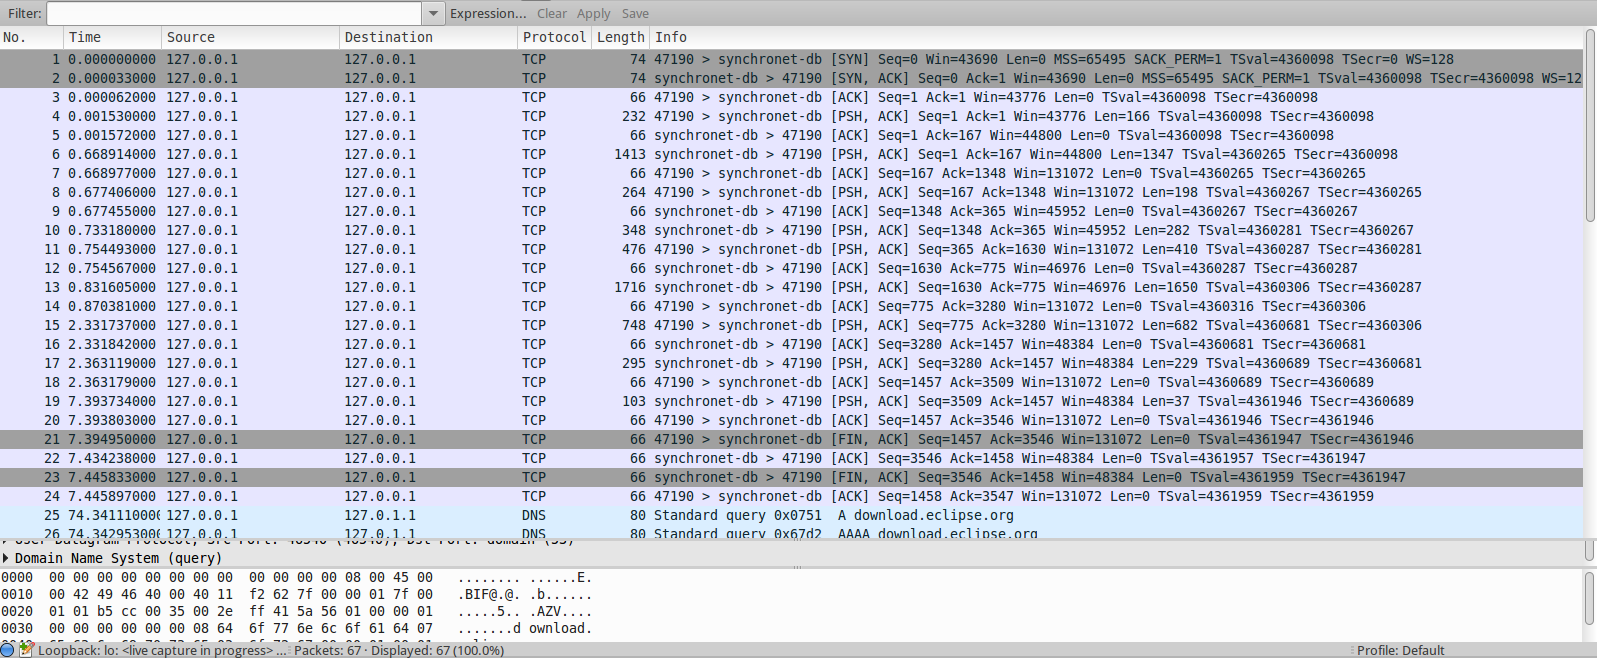
\includegraphics[scale=0.27]{wiresharknetanalysis}}
\caption{WireShark Packet Analysis View}
\end{figure}

\textbf{\textit{Part 3: Develop tailored searches for authentication packets}}
In order to attempt to find the packets responsible for transferring data, the WireShark packet filtering tool will be used. This allows a search query to be entered to filter packets, similar to regular expressions. 
If it is not possible to use this to pick up the packets, then the information is not accessible via intercepting packets, at least not through these means, which implies that it is safe.

The main search queries used will be:
\begin{itemize}
\item Search for requests sent to port 5000 (keystone port):    '\textit{tcp.port eq 5000}' 
\item Search for the Auth Token given from experiment: '\textit{http contains TOKEN}' 
\item Search for header identifier 'X-Auth-Token':      '\textit{http contains "X-Auth-Token"}'
\end{itemize} 

Executing the experiment is simple; for each of the above queries, apply the filter to WireShark, then run the aforementioned Keystone Experiment which authenticates. 

\textbf{Results:} 
Running the first query, as shown in the below figure, returned all the relevant packets first time. 
\begin{figure}[H]
\centering
\fbox{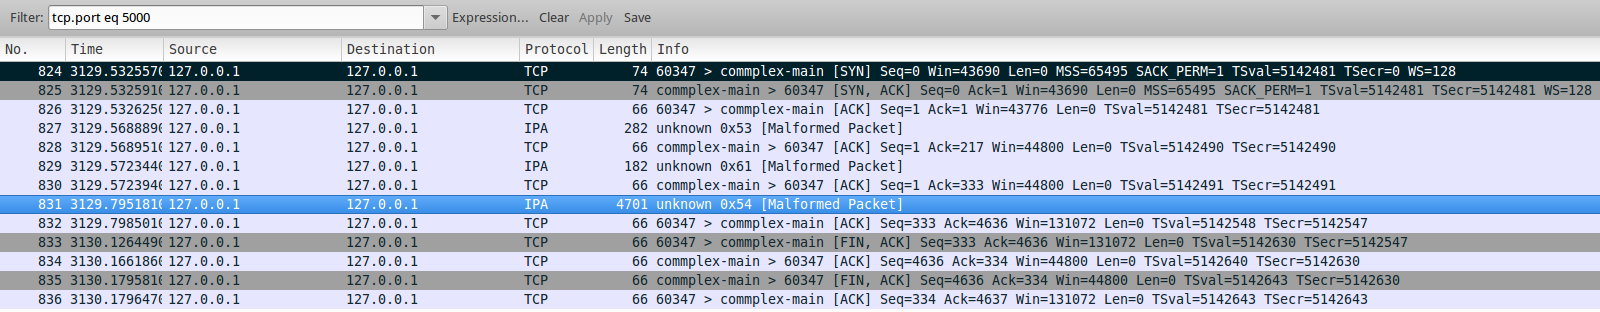
\includegraphics[scale=0.27]{keystone-packet-returned}}
\caption{WireShark Packet Analysis Query results}
\end{figure}

The outcome of this experiment was surprising. As it is possible, and generally default behaviour to run Keystone over HTTP and not HTTPS, it was possible to extract all of the data sent back and forth by the REST Client. This data was extracted using wireshark's 'copy -> bytes -> printable text only' option on the packets, and can be found in the file \textit{extracted-packet-text.txt} in the /logs directory of the final submission. Data captured included username, password, and the returned token, which was then used with the Advanced Rest Client introduced in Appendix E to confirm its validity, shown below: 
\begin{figure}[H]
\centering
\fbox{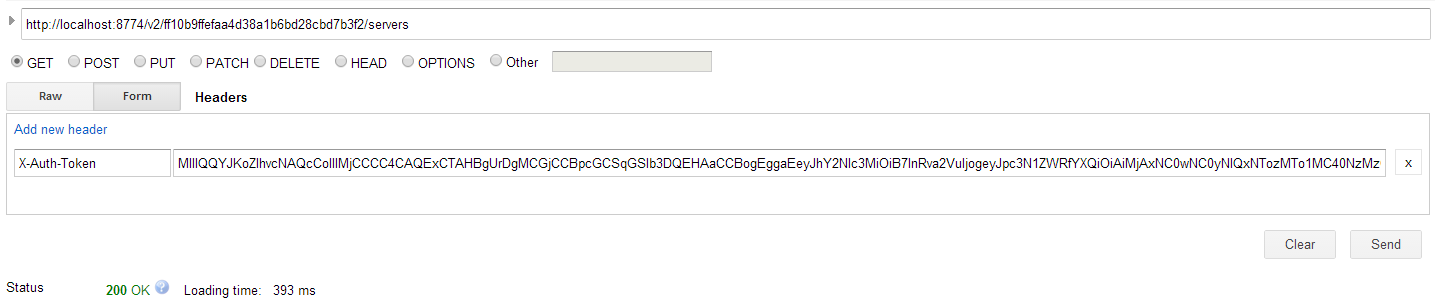
\includegraphics[scale=0.3]{arc-keystone-packet}}
\caption{Running the Advanced Rest Client with the extracted Auth token successfully}
\end{figure}

\textbf{Conclusion:}
In conclusion, it is clear that there is a real problem with security if the administrator does not choose to use HTTPS to communicate with the OpenStack Keystone service. In my personal experience with a similar product, HTTPS was enforced as there does not seem to be a use case where security of an authentication project would not be paramount. It is imperative that any OpenStack deployment used in the real world be configured to use HTTPS, which would not expose this level of information. This is the same for any web site or endpoint using HTTP. 

\textbf{Resources:}
\textit{SimpleKeystoneAuthenticationExperiment.java}
\textit{extracted-packet-text.txt}



\subsection{Nova}

\subsubsection{Experiment N1: Nova Validation}

\textbf{Introduction:}
This experiment will target key functionality of the Nova Compute service, exhibit that functionality, and provide a Java API for other clients to easily interact with the service via its Restful Web Service. 

\textbf{Aims, Considerations \& Metrics:}
The main aim of this experiment is to validate the functionality of Nova, in particular on the cloud testbed. The functionality of Nova of interest includes:

\begin{itemize}
\itemsep0em
\item Creating \& Deleting Servers
\item Obtaining Information on Servers, Flavors \& Images
\item Managing Server \& Image Metadata
\item Rebooting Servers
\item Changing the password of a Server
\end{itemize}

This part of OpenStack is of the utmost importance, as it is core functionality. It will therefore be by far the largest client available, and so will include the largest subset of available functionality, and have the most experiments based upon it. 

The main metrics involved will be a review of the process of developing a client, whether the concepts are too complicated, or whether they could be improved. 

\textbf{Experiment Steps:}
The experiment itself involved a number of large steps, and a number of smaller steps for each of these. The basic development model at a high level was as follows:

\begin{itemize}
\item Identify desirable functionality of Nova via the API reference (v2) \cite{novaref}
\item Using this reference, identify the action required to perform this functionality via REST.
\item Develop the client code to perform this action. 
\item Add this action to the Validator Experiment and run it. 
\item Review the functionality via qualitative metrics such as ease of use, coherency, complexity of client code, etc.
\end{itemize}


\textbf{Development \& Execution:}
The functionality listed above was extracted from the Nova API reference, and an interface \textit{NovaClient} was created to represent this locally. Broadly, this functionality was split into three main groups; Information retrieval, server actions, \& metadata actions. Note, all of these actions require authentication headers mentions in experiment K1. 

\textbf{\textit{Part 1: Information Retrieval}}
This section concerns a number of methods to obtain information about Servers, Images, and Flavors, also referred to here as 'entitites', introduced earlier in this report. Information on these is required to perform any useful action with the Nova project. 
The nova project has a 2-tier pattern for retrieving information in this way. Firstly, there are actions which will retrieve basic information about an entity (i.e. server), usually limited to names, ids and url references. This information can be used to retrieve more detailed information about these entities, for example, getting a server by its id. Nova also provides a method for retrieving details of all the entities of a given type. 
To represent this in Java, the decision was made to design two Java classes to represent each entity. The basic info would be called ENTITYInfo.class, i.e. \textit{ServerInfo}, \textit{ImageInfo}, \textit{FlavorInfo}. The more detailed information, in line with Object Oriented principles, would simply be named for the entity, i.e. \textit{Server}, \textit{Image}, \textit{Flavor}. 
Retrieving this information is performed with GET requests. After the base URL %\begin{verbatim}
\url{http://OPENSTACK_URL:8774/v2/TENANT_ID/}
%\end{verbatim} 
the url extension flavors, servers or images can be used to 'get' basic information on all of these. Further adding 'detail' to the URL provides a similar retrieval of all, and adding a specific id, be it server, image, or flavor, allows a 'get' to retrieve details on a given entity.  

\textbf{\textit{Part 2: Server Actions}}
Nova allows for a number of actions on a server. Firstly, and arguably most importantly, is the creation of a Server. This is achieved by sending a POST request to the URL 
\url{http://OPENSTACK_URL:8774/v2/TENANT_ID/servers},
supplying a reference link for an Image and for a Flavor, described in the previous part.  This creates a server, returning information about the newly created server. 
Deleting a server is as simple as sending a DELETE request to the above link with '/SERVER\_ID' appended. 
The other two actions require sending POST requests to the URL 
\url{http://OPENSTACK_URL:8774/v2/​{tenant_id}​/servers/​{server_id}​/action}.
For rebooting, a simple request body containing the word 'reboot' is sufficient, but for changing a password a new password must be supplied.  

\textbf{\textit{Part 3: Metadata Actions}}
Metadata is extra information that can be added to an Image or a Server using Nova. This information is stored as a simple key-value collection. 
This is very simply retrieved and modified on a per-entity basis. 
Firstly, performing a GET request on the URL 
\url{http://OPENSTACK_URL:8774/v2/TENANT_ID/SERVERS_OR_IMAGES/ENTITY_ID/metadata}
will return each key value pair, and sending metadata in a POST request would update these. Issuing a GET, PUT or DELETE request to this URL plus '/KEY' allows for retrieval, updating or deleting of a specific value by key. 
In java, metadata is represented using the \textit{Map} class from Java's Collections library.
All of this functionality was developed and can be found in the class \textit{NovaClientImpl}, and an experiment using this client was developed, called \textit{NovaValidatorExperiment}. This experiment performs checks that functionality does exactly what is described.  
 
\textbf{Results:} The resulting log file for the experiment can be found in the file \textit{NovaValidatorExperiment.log}. Overall, the experiment was a success. The interface functionality was validated, and a reusable client developed for further use. 

\textbf{Conclusion:} Nova functionality is varied and powerful. From performing asynchronous server operations, to gaining quick access to information regarding resources in OpenStack, the REST API is a useful tool with a logical RESTful request structure. Having the concept of images and flavors in Nova also greatly simplifies the process of performing cross-conceptual tasks such as creating a server from a specified image.
One issue uncovered was the inconsistent representations of entities in JSON format, causing problems for a client. For example, there are 3 different representations of a Server; one with basic information, one with details, and one given after a new server is created. This can become extremely confusing. Similarly, problems were uncovered with timing when no clear indication of job completion or status is given. This was remedied with a number of Utilities, found in the \textit{NovaUtilities} class. 

\textbf{Resources:} \textit{NovaValidatorExperiment} \textit{NovaClient} \textit{NovaClientImpl} \textit{NovaUtils}

\subsubsection{Experiment N2: Nova Extensions Validation}

\textbf{Introduction:} In a similar fashion to the previous experiment, this will target functionality that is part of the Nova 'Extensions API'; this represents functionality above and beyond normal Compute tasks, usually requiring Administrative privileges. The experiment will exhibit this functionality, and provide a means for other clients to do so too. 

\textbf{Aims, Considerations \& Metrics:}
The subset of functionality that is of interest to this project includes:

	\begin{itemize}
	\itemsep0em
	\item Suspend, Resume, Pause, Unpause, Lock, Unlock actions on a Server
	\item Obtaining information on Physical Hosts 
	\end{itemize}

This is mainly due to what the following experiments will aim to achieve, and what tasks are most commonly performed in a virtual infrastructure solution. 
One other consideration will be accessing the extensions API, and whether it should be distinct from the original Nova API Client in the Java Client solution.
Similarly to the previous 'validators', the main points of measurement will involve conceptual complexity of the API, and the code developed to make use of it. 

\textbf{Experiment Steps:}
Following a similar pattern to the previous experiment, the idea is to develop a Java interface for the extensions client \& then implement this using a REST service client. 
Next, an Experiment class will be developed to exhibit this functionality, in order to allow me to form conclusions about the API, and validate its effectiveness on the Cloud testbed.
 
\textbf{Development \& Execution:} In creating a Java interface \textit{NovaExtensionsClient}, the first decision was to link this client to the original Nova client. This is mainly to keep in with the conceptual 'extension' relationship between the two, and because it is likely that the implementations of each will be very similar (e.g. if one is a spring rest client, the other is likely to be too). A method \textit{getNovaExtensionsClient} was added to the \textit{NovaClient} interface to allow this coupling. 
Next, the functionality was tackled in 2 parts.

\textbf{\textit{Part 1: Admin Server Actions}}
Firstly, there are a number of actions that can be performed on a server, such as locking, suspending, or pausing. These all cause the \textit{status} of the Server to change. More information on these statuses can be found in OpenStack's Documentation, specifically in the List Server manual\cite{osserverstatus}.
Developing the requests for each of these, based on the nova extensions API reference \cite{novaextref}, is relatively simple, as they take the following simple JSON form: 
\begin{verbatim}
{
	"ACTION" : "null"
}
\end{verbatim}
where action is the action, such as 'lock' or 'pause'. 
These requests are sent to the URL \url{http://OPENSTACK_URL:8774/​TENANT_ID​/servers/​SERVER_ID​/action} and return no response.

\textbf{\textit{Part 2: Obtaining Host Information}}
Obtaining information about a physical Host can be achieved in 2 ways using the Nova Extensions API. The first of these is to list all Hosts running OpenStack that the tenant can access; this is achieved by sending a GET request to the URL:
	\url{http://OPENSTACK_URL:8774/TENANT_ID/os-hosts}
From this request, a JSON response containing basic information about each host, such as host name, is returned. In order to handle this response, the \textit{HostInfo} class was created. 
The second form of Host information retrieval is achieved by querying one specific Host, usually retrieved with the first technique discussed above. A GET request is sent to the URL :
	\url{http://OPENSTACK_URL:8774/TENANT_ID/os-hosts/HOST_NAME}
	
and this returns a more detailed summary of a Host, defined as a collection of 'Resources' such as CPU. To represent this in Java, a \textit{Host} and \textit{Resource} class was created, with the former containing a List of the latter.  
Note that the use of \textit{HostInfo} and \textit{Host} as two different levels of detail is a pattern that is kept consistent with those mentioned in experiment N1, in order to avoid confusion and make clear the levels of information given. 

\textbf{Results:} The resulting log file can be found in the file \textit{NovaExtensionsValidatorExperiment.log}. The experiment was successful, and functionality was successfully validated. 
\textbf{Conclusion:} The Nova extensions API provides extra functionality which is essential for any advanced Compute setup. In particular, the state change of a Server, such as Suspending or Pausing, allows for a good level of Server manipulation, meaning that resources can be more effectively managed. One piece of functionality that was unable to be used due to a hardware limitation was server migration, but this is indeed part of the Extensions API. 
\textbf{Resources:}  \textit{NovaExtensionsValidatorExperiment.log}, \textit{NovaExtensionsClient}, \textit{NovaExtensionsClientImpl}, \textit{NovaUtils}

\subsubsection{Experiment N3: Server Launch Performance}

\textbf{Introduction:}
This experiment is centred around a very important part of core OpenStack functionality; the launching of Virtual Servers, i.e. Virtual Machines. These are used to provide infrastructure as a service to 'tenants', i.e. users of the virtual infrastructure. 
In assessing OpenStack's capabilities, it is important to see how it performs when starting up Virtual Machines (VMs), and which factors tend to affect this performance. In particular, scale is important; does OpenStack start up VMs more slowly when there is a higher load? Does it take exponentially longer to start up larger VMs? These are some of the questions that this experiment aims to answer. 

\textbf{Aims, Considerations \& Metrics:}
The aim of this experiment is to, as far as is possible, assess the impact of scale on OpenStack's Nova component's ability to create, build and launch Virtual Servers. This is a way of exhibiting OpenStack's ability to be:

\begin{itemize}
\itemsep0em
\item Elastic - it can quickly create \& delete different sizes of server, as is required for a Cloud.
\item Scalable - it can tractably create larger numbers of servers when more are needed.
\item Efficient in Resource Allocation - showing that increasing demand for resources will not cause problems for performance, this implies an efficient allocation system for resources. 
\end{itemize}

The main metric in use here will be Execution time, a Quantitative measure of how long certain operations take. These will be used to spot trends in data, which in turn will be used to form results and conclusions. 

\textbf{Experiment Steps:}
This will be a two part experiment. The first experiment, will work as follows:
\begin{itemize}
\itemsep0em
\item For each Flavor available in the OpenStack configuration:
	\begin{itemize}
	\itemsep0em
	\item From 1 to some value MAX\_INSTANCES:
		\begin{itemize}
		\itemsep0em
		\item start up that number of Servers simultaneously. 
		\item Time how long it takes for every server of that group to be built and in the ACTIVE state. 
		\item Delete all servers 
		\end{itemize}		  
	\end{itemize}
\end{itemize}

This should provide a set of figures showing how much longer it takes OpenStack to build a number of servers when more are added. We should be able to spot some kind of pattern of scalability from these results, and performing with each flavor should show whether the size of VMs is a factor.  

The second experiment will be very similar to the first, with one major difference, and will be carried out as follows:
\begin{itemize}
\itemsep0em
\item For each Flavor available in the OpenStack configuration:
	\begin{itemize}
	\itemsep0em
	\item From 0 to some value MAX\_INSTANCES - 1:
		\begin{itemize}
		\itemsep0em
		\item Create this number of Servers of some homogenous pre-determined flavour, kept consistent throughout the experiment.
		\item Start one Server on top of this, of the current flavor. 
		\item Time how long this one server takes to build. 
		\item Delete all servers. 
		\end{itemize}
	\end{itemize}
\end{itemize}

This experiment will show whether the current load on the OpenStack deployment affects the startup time of one individual Server. Using each different flavor will also show whether the size of VMs is a factor.
NOTE: All timings will be performed multiple times for accurate readings.  

\textbf{Development \& Execution:}
Initially, my thoughts were that the Multiple VM starting experiment should be developed as a CLI script, mainly due to the lack of network based delay, and the ability of a CLI script to repeatedly perform simple actions such as this will little development time. This script \textit{vm-startup.sh} can be found in the deliverable files. Development was fast, but I noticed a problem when gathering results. 
The main issue here was the serial execution time of the script. Using the REST API gives the unique advantage of easily ignoring the response of any request; in other words, everything is a non-blocking operation. In the CLI, without going through extra effort running in a different shell, the operation would block, potentially giving the execution time advantage to those operations starting less machines, and giving unreliable results. 
The decision then was made to create a Java experiment using the REST API, which would be able to parallelise the launch of a number of instances, cutting out any delays in the client skewing results. The experiment can be found in the class \textit{MultiServerStartupExperiment}. Development was straightforward, simply looping through from 1 to MAX\_INSTANCES and repeatedly starting up servers. Utilities such as \textit{waitForMultipleServerBuild}, which repeatedly checked if all servers were finished launching, were created to aid this experiment. This and other static utility methods can be found in the class \textit{NovaUtils}. 
Once this was executed, the next experiment was developed in a similar way, using the Java REST APIs. This can be found in the class \textit{SingleServerStartupExperiment}.

\textbf{Results:}
Graphs representing the execution times for each experiment can be seen below. Note that, for each experiment, resources were too limited to start up certain numbers of VMs \& Flavors, and so the results are incomplete: 

\begin{figure}[H]
\centering
\fbox{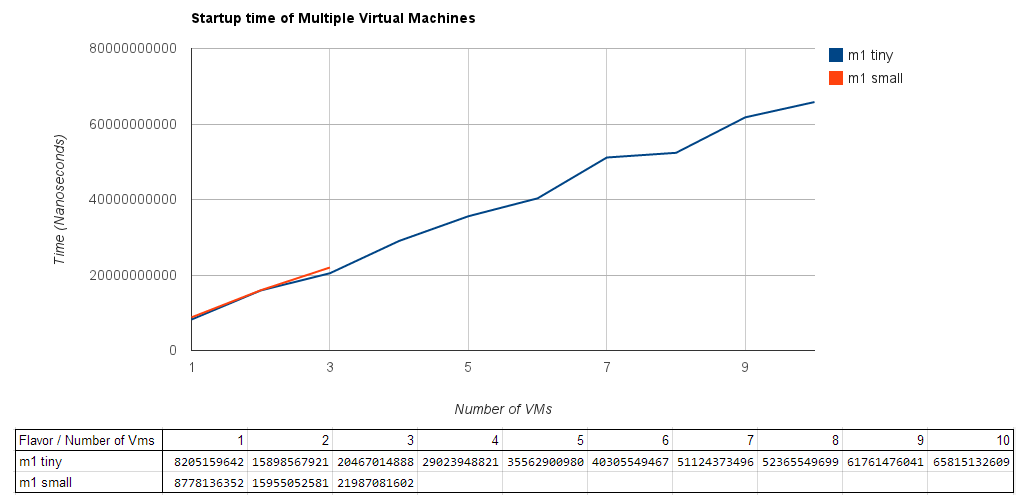
\includegraphics[scale=0.45]{multiple-server-launch-results}}
\caption{Execution times for Multiple Server Launch Experiment, averaged from 30 repetitions.}
\end{figure}

\begin{figure}[H]
\centering
\fbox{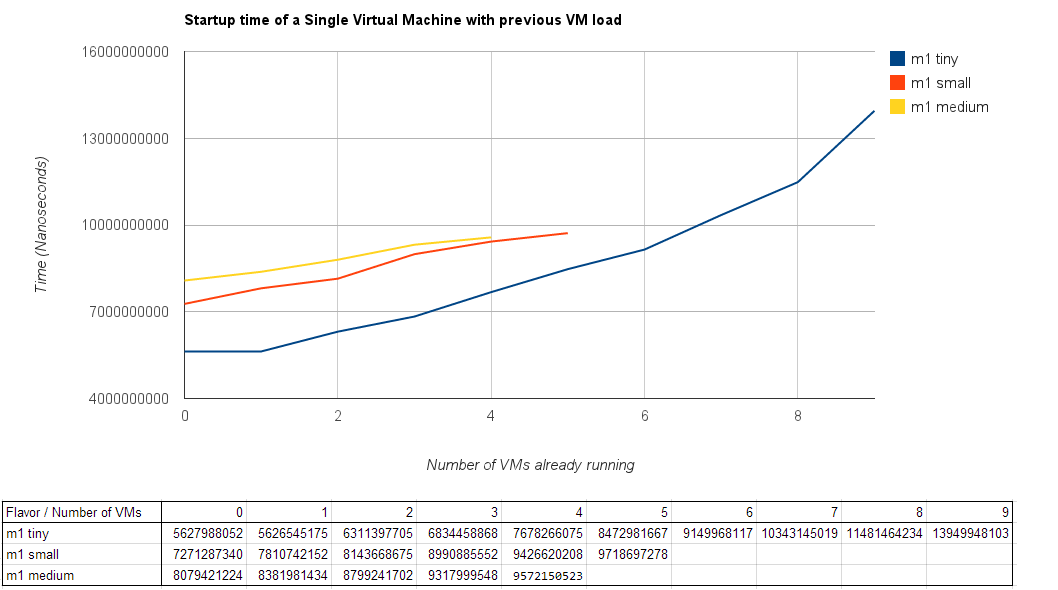
\includegraphics[scale=0.4]{single-vm-launch-results}}
\caption{Execution times for Single Server Launch Experiment, averaged from 30 repetitions.}
\end{figure}


The logs for these experiments can also be found in the /logs folder of the final submission, under the titles \textit{MultiServerStartupExperiment.log} and \textit{SingleServerStartupExperiment.log} respectively.

\textbf{Conclusion:}
Even though the data is limited, a number of conclusions can be drawn from each experiment. 
Firstly, from the first graph, we can see that OpenStack scales very well when starting virtual machines in parallel. The following graph shows how, from 1 VM to 10, adding 1 VM affects execution time, worked out by dividing the current (Current no. VMs) runtime by the previous runtime (Current no. VMs -1).  

\begin{figure}[H]
\centering
\fbox{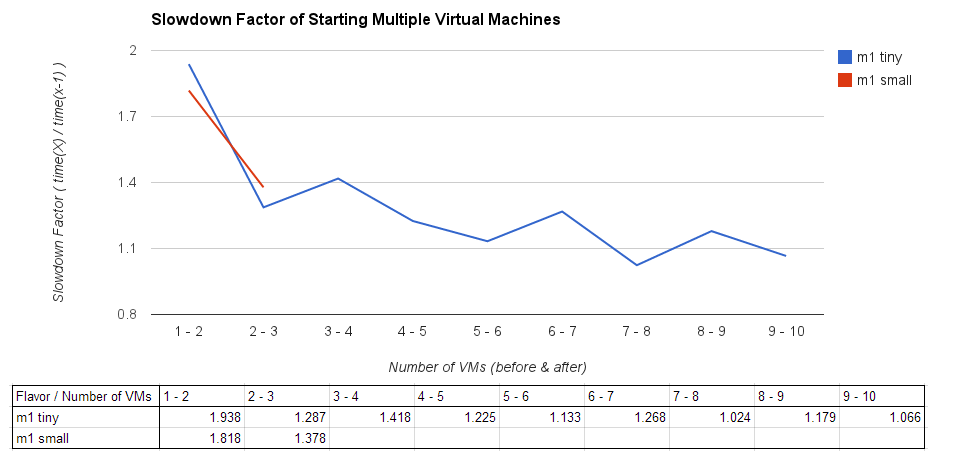
\includegraphics[scale=0.45]{slowdown-factor-multiple-launch}}
\caption{Slowdown factor of execution time from adding a VM for parallel launch}
\end{figure}

This diagram, using a concept similar to speedup\cite{speedup}, clearly indicates that OpenStack scales very well in terms of simultaneously launching Server VMs, even reducing the factor of slow down when VM load is higher. The gradient of the original curve shows this, it does not change greatly between 1 and 2 VMs, and 9 and 10. Similarly, flavor size does not appear to affect either the raw startup time, or in fact the factor of execution time increased, implying that OpenStack's ability to scale in terms of VM size is also very good. 
The second original graph shows similarly that OpenStack scales extremely well when creating single VMs with additional load on the Nova component. Starting VMs after already running more VMs does have a noticeable affect on performance however, as does flavor, but it is important to note that the gradient of each line is not dissimilar; this means that in terms of scaling, the execution slows down at a similar rate even when flavor size is larger. One statistic that is concerning is the change in gradient of the blue line, showing that the execution time difference between 9 and 10 VMs is relatively much larger than between 1 and 2 VMs. A slowdown diagram similar to that shown above illustrates this - the slowdown line for m1 tiny spikes as load increases:

\begin{figure}[H]
\centering
\fbox{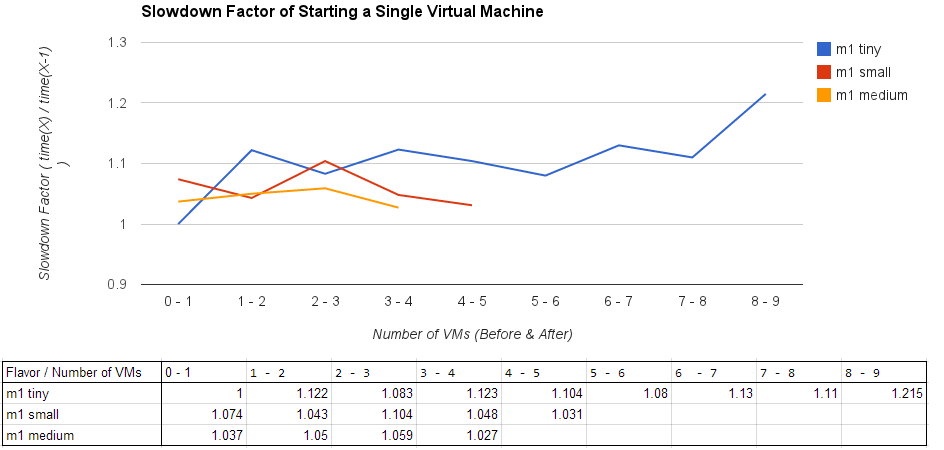
\includegraphics[scale=0.44]{slowdown-factor-single-launch}}
\caption{Slowdown factor of execution time from adding a VM load for single launch}
\end{figure}

Overall, these tests show that OpenStack has impressive scaling capabilities in terms of VM size, current VM load, and parallel VM launch. There are some issues, but further investigation on this would be required. 

\textbf{Resources:}
For the first part of the experiment, see \textit{MultiServerStartupExperiment.java} \& \textit{vm-startup-experiment.sh} in the final submission files. \\
For the second part, see \textit{SingleServerStartupExperiment.java} in the final submission files. 

\subsubsection{Experiment N4: Server Status Analysis}
\textbf{Introduction:}
Servers in OpenStack can have a number of Statuses, or States. When a Server is not active, there are a number of states it can be put in until it is needed again, in order to save energy, or compute capacity. In OpenStack, servers can be Paused, Suspended or Locked. 

\textbf{Aims, Considerations \& Metrics:}
Pausing a server stores it in RAM, whereas Suspending a server stores it on disk.\cite{nova-admin-server}. Locking the server just disallows certain operations to be performed on it. The idea behind this experiment is to see firstly which of these operations is fastest, and so generally preferred, and also whether the size of a Virtual Machine flavour has any effect on these operations. The metric to compare these will of course be execution time, averaged over a number of executions. 
I would expect suspending to be much slower than the other two, mainly due to its use of secondary storage. 

\textbf{Experiment Steps:} 
The experiment steps are as follows:
\begin{itemize}
\item For each Flavor:
	\begin{itemize}
	\item Create Server of size Flavor
	\item Perform each action couple {Pause, Unpause}, {Suspend, Resume}, {Lock, Unlock} and record times of each, REPETITIONS times.
	\item Take averages of these times 
	\end{itemize}
\end{itemize}
\textbf{Development \& Execution:}
Development of this experiment was relatively straightforward. The class \textit{ServerStatusPerformanceExperiment} was created, with code to perform the steps above, by looping through each flavor and repeatedly making calls to the Nova Extensions API to perform server admin actions such as pausing a server. A utility was created in the \textit{NovaUtils} class called \textit{waitForServerStatus} which allowed waiting for servers to change to the desired state, e.g. PAUSED, SUSPENDED. 

\textbf{Results:}
Below are the results of this experiment as a Bar chart. This shows the averaged execution time for each server operation, grouped by flavor size. 
\begin{figure}[H]
\centering
\fbox{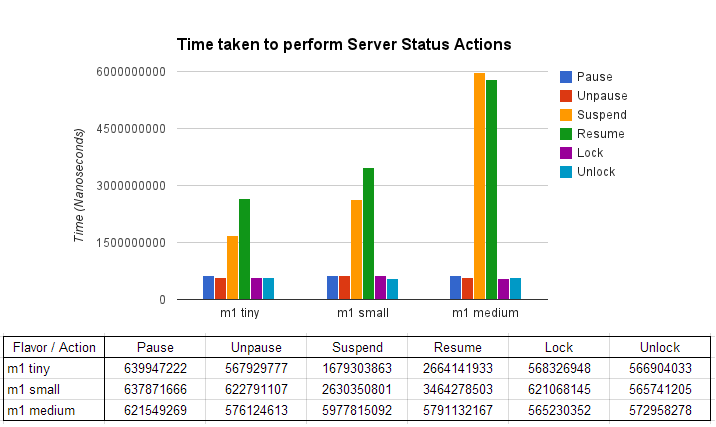
\includegraphics[scale=0.62]{server-status-results}}
\caption{Execution times of Server Admin Operations for different VM sizes}
\end{figure}
\textbf{Conclusion:}
As expected, these results firstly show that the Suspend \& Resume operations take a significant amount of time longer than the other operations, and this is most likely due to the overhead of writing to disk, especially with commodity hardware. The other actions only deal with operations in RAM, and this is known to be significantly faster.  \\
One surprising result here was the lack of increase in execution times in Locking \& Pausing operations as flavor size increases. As expected, Suspending \& Resuming a server takes much longer as flavor size increases, as more information is written to the disk. This pattern is not true however for the other operations, most likely due to writing to memory not having the same overhead as to disk. This of course has the disadvantage of being limited in capability; much larger VMs can be written to disk than can be written to RAM, especially in a system with a lot of load.  
We can conclude from this that, in many cases, locking and pausing a server is a much faster operation, but will still have an impact on RAM, and so Suspending a server may be the only option; in this case, one must be prepared for a long wait to write to disk, which appears to get exponentially larger as the VM size increases. 

\textbf{Resources:}
\textit{ServerStatusPerformanceExperiment}, \textit{NovaUtils}, \textit{ServerStatusPerformanceExperiment.log}
\chapter{Evaluation}
\label{CHAP_SIXTH}
\centerline{\rule{149mm}{.02in}}
\vspace{2cm}

\section{Implementation / Results Summary}
\subsection{Qualitative Analysis}

The main result of the qualitative analysis was of great compliment to OpenStack. Overall, it appears to be a well designed system, which exhibits all of the desired characteristics of a Cloud and of a Virtual Infrastructure Manager. By analysing the architecture and design of the system using standard metrics such as cohesion, it was possible to form a coherent conclusion about OpenStack which would provide useful perspective on it's workings. The below figure shows which of the desired characteristics of a VIM and of a cloud are covered by which components of OpenStack, giving an overview of \textit{how} OpenStack provides the services and capabilities required of each: 
\begin{figure}[ht]
\centering
\fbox{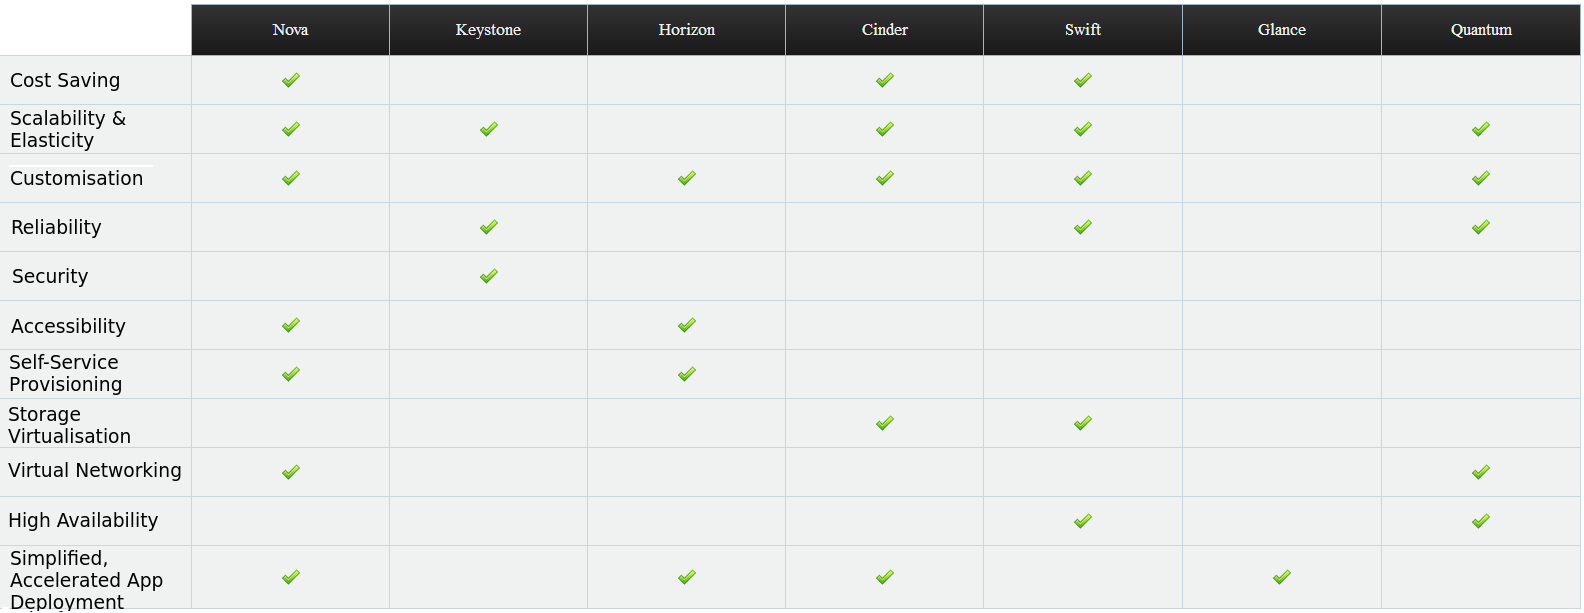
\includegraphics[scale=0.24]{cloud-characteristic-comparison}}
\caption{Table showing which Desired Cloud \& VIM Characteristics are exhibited by which OpenStack components, based on this project's Qualitative report}
\end{figure}
Overall, in terms of cohesion and coupling, it was found that OpenStack has a very well defined modular design, which allows for components to be highly cohesive and act as services to the other components, together forming an effective system. This was shown in most components by the narrow aims and capabilities of each module. For example, the Glance Image service would exclusively handle bootable VM Images, and try not to go beyond that. 
However, in places this granularity did cause some problems, as there seemed to be some conflict between the decoupled mentality, and the ability to make certain modules self-sufficient. The most salient example of this was the Nova module, which, despite being a specialised Virtual Machine Instance management module, had its own concepts and definitions of VM images and networks, meaning that it had very low cohesion. The idea here was clearly to allow basic setups based around the Keystone and Nova modules, meaning there was no heavy dependency on other modules to provide services, but in the end this caused inconsistencies in the application when those modules handling each were involved. A great example of this was the REST APIs for the Nova \& Glance components. each had its own definition of what an Image was, and for a client, it became increasingly confusing to actually use both of these modules together. In the end, the result was that the Glance service was not relied on, as nova provided its own version of this functionality. 
These drawbacks are far outweighed by the flexibility and customisation provided by the loosely-couple architecture, and the use of standards-compliant RESTful APIs make interaction between components extremely simple. It appears, from this analysis at least, that the designers of OpenStack made the right decision to go in a new direction and go with a fine granularity based approach, as this provides a number of advantages for clients deploying their own instances of OpenStack. 
Another feather in the cap of OpenStack uncovered by this analysis was the sheer level of customisation and functionality available through its various components. Even given the high level of expectation in terms of functionality on a system which provides cloud infrastructure, OpenStack delivers; advanced features such as Software Defined Networking, Virtual Storage, and high availability object storage are provided, meaning that, on paper, it is a perfectly viable cloud solution. 

 

\subsection{Qualitative \& Quantitative Experiments}
The results of the 'Exploring OpenStack through Experimentation' section were very mixed. In some cases, experimentation was very informative, and brought useful information to light. A 'conclusion' section can be found at the end of each given experiment, explaining the results and how they are interpreted. In this section, I will reflect on the overall results of running experiments; what was achieved, whether the experiments were useful, and what they mean for somebody using OpenStack. \\
The first 'type' of experiment ran, of which there were three (K1, N1, N2), were the 'Validator Experiments', the aim of these being to not only validate OpenStack functionality, but also to develop a reusable client for this functionality, and even to give a brief review of it, in terms of metrics such as conceptual complexity, or code complexity. These experiments were very successful. For each piece of functionality, the experiments provide background information about how they work, and then guide the reader through the development process for both the functionality itself and the validator experiment, with code then being provided as a guide for further development, as well as a re-usable testing component. All of this is valuable to somebody wishing to learn how to interact with OpenStack, and even somebody wishing to validate their own deployment. In each case, the developed functionality worked well, and this functionality was then cleared for use in the later quantitative experiments.   It is my view that this level of useful product justifies the 'validation' approach.\\
The 'Quantitative Performance Experiments', of which there were two (N3, N4), provided a totally different angle for OpenStack analysis. These were much more practical, and were devised in the hopes of testing OpenStack for characteristics such as Scalability, Elasticity, and Efficient Resource Allocation. These experiments proved to be much more challenging to execute, mainly due to unexpected resource limitations, discussed later in this chapter (Unexpected Issues/Limitations). These limitations meant that many of the results, particularly for the Server Launch Experiments, were partial, and so it was difficult to effectively draw conclusions from the results in a reliable manner. Due to this, the conclusions made were kept limited, and the Experiments provided as re-usable code for those users with larger deployments to try for themselves. Another issue was with the interpretation of results. In some cases, certain behaviour could only be observed, and not necessarily explained, due to a lack of time and lack of knowledge of the inner workings of OpenStack. Despite these issues, the experiments, along with experiment K2, a practical security test, uncovered some very useful information, which can be found at the end of each experiment write up under the 'Conclusion' heading, and so I believe that they were still worth executing. It would have been a good idea to design experiments with the resource limits in mind, but unfortunately I was not aware of them at design time, and such a drastic change in approach was not possible at such short notice. \\
Some interesting findings from these experiments are listed below:
\begin{itemize}
\item The OpenStack Keystone Identity service can be deployed 'unsecured' over plain HTTP, which is VERY dangerous in multi-tenant deployments. An experiment successfully intercepted packets containing private authentication information.
\item OpenStack Nova Compute scales well with respect to number of VMs launched simultaneously and also with respect to launching a VM with current load, although less so.
\item OpenStack Nova Compute does a good job of scaling in terms of 'Flavor Size' or VM resource allocation size, as results show many operations are not slowed down at the same rate as the increase in size of the VM. For example, m1. medium is approximately 4x the size of m1 small, and yet operations are not 4 times slower. 
\item Suspending a Server is a lower performance, less scalable solution for stopping the running of a server when compared to pausing and locking a server; it is however necessary if RAM is limited on the cluster.  
\end{itemize}

\subsection{Delivered OpenStack Client}
This project has delivered a working OpenStack client. The first main aim of this client was of course, to interact with OpenStack's REST APIs to perform various actions. In this sense, it was of course successful, in that it performed multiple actions on 3 of OpenStack's components; Nova, Keystone and Glance, with a 100\% success rate. This client functionality was then exposed through a number of Java interfaces in order to be used by any client, or experiment, that requires it.\\
The consequence of this is the satisfaction of the second, and arguably most important aim of the client; to validate OpenStack functionality. Experiments were successfully created using the aforementioned interfaces, and tested the effects of each successful interaction. In this way, we validated that OpenStack behaves as expected, and also does so on the Leeds Test Bed deployment, something which is a useful basis for further experimentation. \\
One of the greatest achievements of this code however is that it is designed to be easily re-usable. The use of Spring's JavaBean XML definitions for OpenStack configuration and Experiments allows any OpenStack setup and written experiments to be executed. A base class for new experiments which allows them to hook into this system is also provided; all of this is explained in Appendix E. From this, it is clear that what has been delivered is a means to use OpenStack, create experiments for further testing, execute experiments old or new, and learn about how to develop for the REST APIs. I would therefore deem this an overall success. \\
However, there were some issues with this deliverable. Firstly, as with the  experiments, it was not possible to cover much of OpenStack, due to the various limitations discussed later in this chapter. Secondly, due to time constraints, full and expanded documentation was not possible, and so much of the code must be read and understood without much guidance.  Perhaps the biggest problem with the development was due to the nature of REST APIs; asynchronous requests created certain delays which are not handled by the REST API. This did seem to be a failing of the design of the API, not including some kind of job context which would be used to query the status of a job. The closest thing to this was the status code of each request, but a 200 OK code would not guarantee there was not an issue, and utilities like those in the \textit{NovaUtils} class were necessary to make up for this. For example, if a Server is launched, a 200 OK response code does not imply the server is not in 'Error' state. There would also be problems that if a Server was deleted, it would still show up if a request to list active servers was sent, as the delete operation was not completed. The utility methods \textit{waitForServerState} and \textit{waitForServerDelete} were created to tackle each of these respectively.

\subsection{Conclusion}

From the discussion above, I would suggest that the results and deliverables from this project have provided useful and varied information about OpenStack. Through the Qualitative report, there is good coverage of OpenStack despite limitations, and I believe that it would really help a user learn about it at a high level. To complement this, and make up for its natural 'high level information only' limitation, experiments both qualitative and quantitative provide more specific details about OpenStack's APIs, functionality and performance in a real deployment. Although not all of OpenStack was covered, arguably its two most vital parts, Keystone and Nova, were. The experiments have been delivered in code form, along with a code deliverable which allows for anyone to set up and execute them, plus their own experiments, with minimal configuration. It is plain to see that I have not only experimented, but paved the way for further experimentation and development in this area. \\
Overall, it appears to have been a good to have three separate deliverables. Each of these could of course be improved upon, and that is certainly something for the future which will be discussed later in this chapter, but overall, I am happy that enough information and guidance has been delivered concerning OpenStack. 

\section{Comparison with other Evaluations}

As part of the Evaluation of this Evaluation of OpenStack, it is important to compare it against the previous evaluations which were highlighted in the background research for this project. In this way, we can ascertain whether this project has added any value to the domain, and have some point of comparison to gauge the relative success of the project. 

\subsection{ETF Evaluation}
In some ways, the ETF evaluation\cite{etfevaluation} \& this one bear similarity. For example, both initially aim to provide a basic overview of the OpenStack technology; the ETF evaluation starts with a list of relevant components of OpenStack, to give the high level view, as does this. They are also similar in that they both aim to provide insight and guidance as to the use of OpenStack, something at least in part covered in this evaluation. Where these two differ, however, is that there is a particular focus on User Experience and Deployment in the ETF evaluation, something not covered in this evaluation. On the other hand, this evaluation covers aspects of OpenStack that the ETF did not, such as the performance of the Nova compute component \& comparing interfaces to OpenStack. In this sense, I believe this evaluation does cover new ground, and provide new information and knowledge.  
Similarly, it seems the approach of my evaluation was much more in depth than that of the ETF; certain aspects, such as 'architecture', which were analysed in depth using formal metrics in this report, were covered in a one sentence answer by the ETF. In general, this evaluation is longer and more in depth, giving me confidence that this report will be useful. 
The final difference spotted was the lack of development involved in the ETF evaluation. There is no evidence of programmatic experimentation being documented by their evaluation. Furthermore, a toolset ready made from Eucalyptus, a competitor project, was used instead of the approach of this project, which was to develop a client specifically for OpenStack. 
One thing this has shown me is that I may have been able to get more done in terms of experimentation and analysis if I too had used a ready made tool to interact with OpenStack. This is perhaps a failing on my part, not knowing the true benefit of the standards-compliant REST APIs OpenStack employs. \\
In terms of results consistency, there were some joint findings. The main example of this is the issue of security, where both evaluations found, albeit in different ways, that there was some issue with the identity service. 

\subsection{CERN Evaluation}
Before a comparison is made between the CERN evaluation\cite{cernevaluation} mentioned, it is important to mention that the actual findings of this report were not made available, and so what will be compared is the \textit{approach} of the CERN evaluation, not its results. 
In aims and objectives, it appears that the CERN evaluation was heavily focussed on the validation of OpenStack's functionality; something that was also covered in this evaluation. Another common goal of each project was the practical use of OpenStack as a form of analysis and this validation. In this sense, CERN's evaluation seems to go into further detail than this evaluation, which is more focussed on basic usage. I believe this is mainly down to the resources allocated to each project; it was difficult to perform advanced manipulation of the resources given, as described in the  'Unexplained issues/limitations' section of this evaluation. Despite this, I still believe that the 'guide' style of this project's validation is useful, and it does cover some functionality that is not highlighted by CERN, such as server metadata and keystone authentication. 
To further compare the two, it is worth noting that CERN had some qualitative evaluation planned, but the focus was more on administrative functionality like provisioning hardware and managing the VM lifecycle, not analysis of the design and architecture of OpenStack, as in this evaluation, so this project does cover new ground in this sense. However, CERN did not include any form of pure quantitative evaluation, for example, performance testing, nor did they intend to produce a code deliverable similar to the REST Client delivered here. In this way, my evaluation is providing new value to the domain. One aspect of the CERN evaluation I could really learn from is the great level of planning. Every step of the project was clearly mapped out early on, something which was not the same for this evaluation, although the resources and aims of this project were always less clear from the off. Due to this, it is my view that the CERN evaluation was a better structured, more organised approach to OpenStack's evaluation.

\subsection{Conclusion}
Overall, it seems that this evaluation of OpenStack has provided some real value to the OpenStack knowledge base, and hopefully to members of the ASCETiC team, and other readers. The coverage of OpenStack was high qualitatively, but some detailed analysis was still possible quantitatively, providing a good balance of the level of information. I feel that in places, this project has covered new ground, and gone into more detail on other areas, such as programmatic experimentation. 

Provided below is a table comparing what is provided by each evaluation:

\begin{figure}[H]
\centering
\fbox{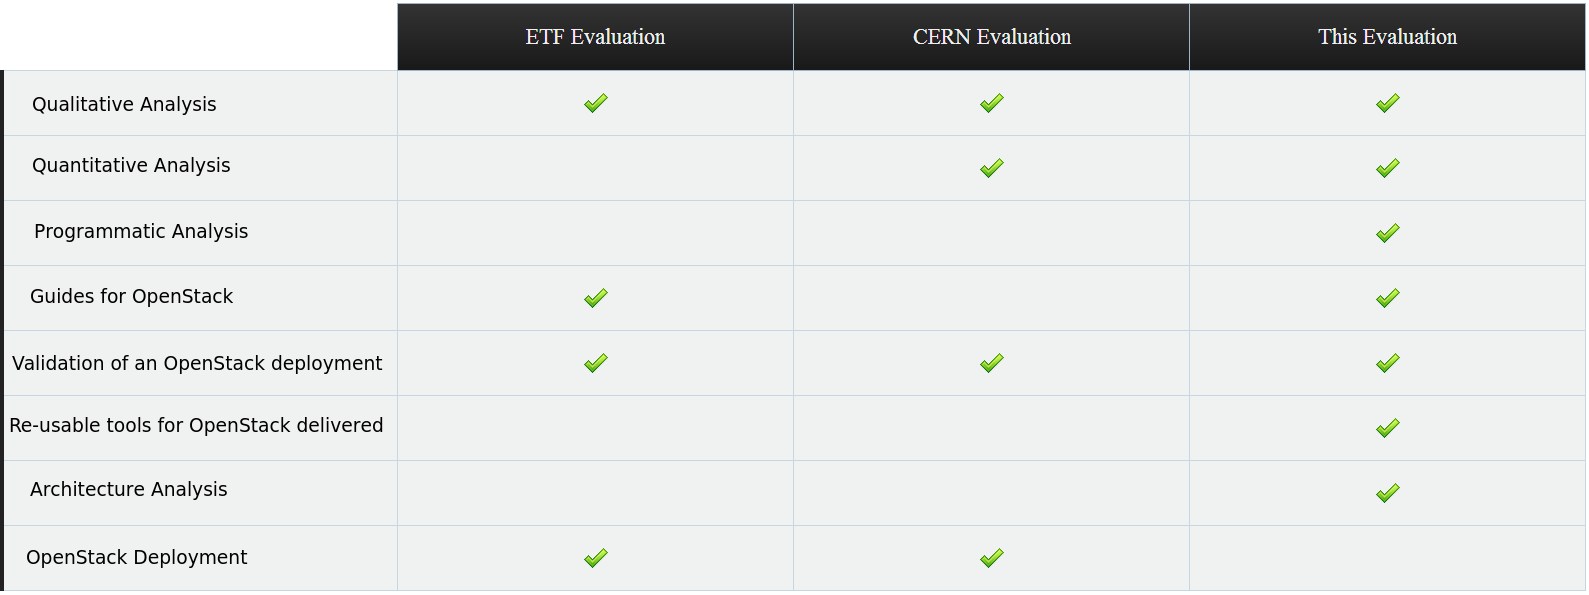
\includegraphics[scale=0.24]{evaluation-comparison-table}}
\caption{Table showing which aspects of Evaluation are covered in each evaluation, comparing this project with 2 previous evaluations.}
\end{figure}

I am happy with the performance of my evaluation in this table, as it shows that it covered a great number of aspects which one or the other previous evaluation did not, and in some cases, new ground entirely. In a space which is relatively new, it may indeed be one of the first of these reports of its kind. One issue I have had with the results is perhaps the 'jack of all trades' approach; by this I mean that qualitative analysis, quantitative experimentation and software development were all combined into the project, where maybe it would have been possible to focus on one. This approach came from a couple of real aims; firstly, was to cover new ground, especially in the practical, quantitative space. Given the limitations discussed later in this chapter, and the aim to provide guidance to OpenStack, it made a lot of sense to infuse example code and analysis of OpenStack with this too, to give an example of how to deal with OpenStack in a number of ways, practically and theoretically. I really feel like the project was successful in this respect.  

\section{Project Management \& Outcome}
\subsection{Aims \& Objectives}
In light of the outcomes of this project, I am a firm believer that the aims \& objectives of this project were well set, and were reasonably difficult, but still achievable. Having objectives as varied as those for this project was always going to be a risk; it was hard to know how long each would take, given that there was no clear information about OpenStack or its use at the time. The idea then was to attempt to link these objectives together, so that much of the work would in some way contribute to multiple aims. For example, the objective of producing implementations for programmatic tests and the other to produce re-usable software were always intended to be intertwined, and the resulting REST Client reflects this. The aims \& objectives of the project were not necessarily clear at the start of the project, however, and were slightly modified as a response to the feedback from my mid-project report. The feedback stated that the objectives were perhaps unclear or vague, and so I felt it important to consider 'what is an evaluation'? This process can be read at the end of the 'Background Research' section, where the plan for evaluation of OpenStack is explained. \\
In conclusion, I am happy with the way the objectives looked after the initial re-think. Initially, they were perhaps too vague, such as 'Produce an evaluation report of OpenStack' with no explanation. Changing this to 'Produce a Qualitative Architecture \& Functionality Analysis' meant that it was clear what the aim of the deliverable was, and these changes as a whole helped to really form the identity of the project. 

\subsection{Project Methodology}
As mentioned in Chapter 1 of this report, the approach to this project was defined in 2 ways. Firstly, it would take an agile approach, meaning development would be incremental and formed as it was developed, using rapid prototyping techniques. Secondly, it would be split into four phases; research, implementation, conclusion and evaluation.  \\
The agile approach in itself has proved itself as the correct choice for this type of project. As the objectives and amount of work to be done were unclear, the approach of developing ever-improving prototypes meant that the code and report were not sensitive to changes in the project definition at any one time, and were always ready to be delivered if time ran out. Working in sprints personally helped my focus, and whole experiments could be completed in short bursts of effort, helping to organise the project work effectively. The iterative approach is not well reflected in the resuts write-up, and this is mainly because the iterations were very small and part of the developemnt process, not something I deemed worthy of write-up.  Splitting the work into 'phases' went hand in hand with the approach just mentioned. I was able to give myself free reign to work on what was needed, and be incredibly flexible, as long as project milestones were hit. All research was completed before implementation began, and all implementation finished before conclusions were drawn, etc. Within each of these phases, what work was to be done was kept loosely defined, with a list of work to do always available. This was particularly helpful due to the learning nature of the project. If I was stuck on developing the report, I could switch to developing the code deliverable, and this often taught me more about what I needed to know about OpenStack for the report. \\
Neither of these approaches were without problem. The approaches were indeed flexible, but in some cases this meant being unorganised, and often it was easy to lose track of what work was completed and needed completion, especially after a break from work. Despite this, the outcome of the project justifies the approach in my opinion, and I am happy that the work was consistently productive throghout, partly down to these approaches. 

\subsection{Project \& Time Management}
The way the project was managed has no doubt helped to make it successful. The approach in general was to work on an ad-hoc, flexible basis so as to simultaneously work on multiple deliverables, and this put a lot of emphasis on how my time and the workload were managed. 
A useful tool I used was a simple Note Taking application on my laptop. When work was to be done, this would be written up as a task list, and struck off when it was completed. By looking through this and the work, it was easy for me to guage where the most work needed to be done, and from this I could decide where to place my effort. 
Tools such as version control on this LateX project and every code deliverable meant that work could be completed anywhere, on multiple machines at home or university, something which had a huge effect on my time management, as I could work whenever I needed to without waiting, and more effectively and flexibly perform sprints.
My approach was tested part-way through the project when the requirements changed, and so much of the time and energy that would be spent on work by my GANTT chart were spent almost 're-defining' the project. It is testament to the methodology and the management of the project that this did not affect the final outcome, and putting in more hours, and perhaps scaling back on the more advanced objectives, solved this issue. 
In terms of time management, I do think there are some things I could have improved upon. For example, the testing of prototypes was not something I spent enough time on, and this often meant spending more time fixing problems in the code than was necessary. Problems like this were down to my own failings, wanting to do the more exciting work most of the time, and neglecting other work. Unlike many projects, this report was written as the project went on, and iteratively developed like the other deliverables, as opposed to just being written up at the end, meaning I could ensure a slightly higher level of quality than there would have been if it were rushed at the end. 
Due to changes in the project, and a few personal problems, the look of my GANTT chart did change, mainly taking longer and with planning in the middle. The updated chart can be found in Appendix F: 

\subsection{Unexpected Issues/Limitations}
\begin{itemize}
\item Cinder \& Swift could not be installed due to a lack of LVM technology on servers.
\item Neutron could not be installed due to incompatibility with the Leeds network
\item Hardware resources were limited to 2 machines, 8gb RAM, 8 cores. 
\item Didn't have full admin access to OpenStack until late in the project
\item Server Migration could not be performed as both OpenStack servers had different architectures. 
\item Time taken to deploy OpenStack ate into early project time.
\item No comparable setup was available to evaluate another product in comparison quantitatively. 
\item Documentation for OpenStack was often found lacking, especially for feature explanations.
\end{itemize}

\section{Future work} 
\subsection{Further Research}


The possibility of future work in this area is almost limitless due to the size of OpenStack, but with more time I would have focussed on first including the final two missing components from the qualitative analysis, Ceilometer and Heat\cite{openstacksoftware} to improve coverage. Next, I would have performed more investigation of the design, including new metrics such as static code analysis, bug count and code coverage. Finally, a full architecture and capability analysis comparison with another project such as OpenNebula is something I would have aimed for, in order to assess OpenStack vs the competition.

\subsection{Further Experiments}
The first work that follows from this is to of course run the designed experiments on a larger OpenStack deployment, to get some more useful results at larger scale. Following this, I would have aimed to have the other OpenStack components, such as Cinder, installed, and validator experiments created for each, to validate their functionality. Once validated, the possibility for experimentation is endless, but some key experiments I aimed for were performance analysis of server migration and scalability of storage creation using Cinder. I also aimed to compare the launch of a VM when using a snapshot vs using a bootable VM image. Luckily, the way the experiment framework is written allows for these types of experiments to be developed relatively easily, and this was in mind when designing the framework. 

\subsection{Improving the REST Client library}
Before talking about the next parts of this tool to be developed, it is important to mention a couple of improvements that could be made. Firstly, updating the current clients to new APIs would be useful, as some were just being released as the project went on. Secondly, the authentication system could be improved to include validation of a token and knowledge of when tokens time out; much information is provided with a response from Keystone, such as timeout date, but this project only uses the token itself at this point. Finally, the documentation of the code could be massively improved, and is not at its best due to the rapid development approach taken. Further work would of course include developing client functionality for other components in order to create experiments, but also improvements to the Exception handling of the project, in order to more effectively handle errors with OpenStack. Further utilities would also need to be created in order to handle any other issues with new REST APIs. 

\section{Conclusion}

This chapter has aimed at evaluating the work performed in the previous chapter by first summing up the results and findings, and then assessing those results, through comparison with previous similar projects, and by other means.  Furthermore, it has critically evaluated the project approach and management as a whole, considering which aspects were successful and unsuccessful, and finally, what work would have been performed had there been more time. The idea of this chapter was to give some insight into the nature of the project, what it was like to work on, and what issues were discovered and potentially overcome. \\

The next, and final chapter of this report considers whether the initial aims and objectives of the project have been met or exceeded, as this is one of the most salient indicators of success.    
\chapter{Conclusion}
\label{CHAP_SEVENTH}
\centerline{\rule{149mm}{.02in}}
\vspace{2cm}

In order to guage the success of the project, it is important to look at it's minimum requirements. The first requirement, a \underline{literature review} of the background material relevant to the project, was successfully met, and now makes up the 'Background Research' section of this report. The literature review proved extremely helpful in learning around the domain and even planning the approach to evaluating OpenStack. At least \underline{1 programmatic experiment plus 3 designed experiments} was also expected. This objective has been met and exceeded by far, with at least 6 re-usable experiments designed, with 5 of these being 'programmatic' i.e. using the REST APIs. Next, a \underline{Qualitative Evaluation report} was required, and this is delivered in part 1 of the 'Design \& Implementation' section, as a report on OpenStack architecture, design and capability; again, the target was successfully met. Similarly, a large \underline{re-usable software component} has been delivered in the form of a Spring based REST Client for OpenStack. \underline{Evaluation} of the project itself can be found in Chapter 4. \\
Clearly, the minimum requirements of this project, deemed reasonable by the project assessor, have been far exceeded in this project; furthermore, the production of an \underline{Experiment Framework}, listed as a possible extension, is built in to the REST client, meaning this extra objective was also achieved. The design of the Spring application which provides this can also be easily \underline{used with other configurations}, meaning that this project easily allows another possible extension, the running of experiments with different configurations; all that prevented this happening during the project was a lack of physical resources, and time to reconfigure the OpenStack environment. In terms of the Aims \& Objectives themselves, what is produced is very much in line with them, and the projected deliverables have all been matched and will be delivered with this report. It is for this reason that I would personally deem the project successful, based on it's initial, and in my opinion, ambitious aims. 

\addcontentsline{toc}{chapter}{\numberline { }Bibliography}
\bibliographystyle{unsrt}
\bibliography{refs}      % include the bibliography

\appendix                % include the appendices
\chapter{Personal Reflection}
\centerline{\rule{149mm}{.02in}}
\vspace{2cm}

I initially chose this project due to a vested interest in the Cloud Computing Domain, from previous work and my planned career path. I thought that, as I had interest in the area, I would be happy to work long hours to achieve a greater level of knowledge and contribution to the field. I was at first concerned that I had made a mistake in choosing in this way, as many consider the Final Year Project a way of exploring and learning something which you may not have another chance to look at, something specific to research or academic environments. This fear was quickly quelled as I realised the enormity of the task ahead; I had definitely not picked the easy option. The work required of me throughout the project stretched me to trying new things, learning new techniques, and ultimately adapting to a completely different style of work. In retrospect, I truly believe I made the right choice with this project, and I was correct in that when the work became tiresome or long winded, it was my passion for the involved technology that spurred me on to work through it. 
In addition to the subject matter, the style of project work suited me well. There was a nice mix of research and development, meaning I could develop my skills in a number of key areas, something which will no doubt benefit me in the future.    \\

I had little experience both planning and managing a real project before this one. The nature of most work in university has led me to perform work in short, intense bursts, committed to an upcoming deadline. Planning a three month project then was something completely different for me, requiring a much more organised, slow and steady approach. In my opinion, I handled this new challenge well; the use of techniques such as a GANTT chart and setting milestones allowed me to pace myself, producing a steady stream of good quality work. It was however not easy, as my natural tendency is to complete work very close to the deadline; I was very anxious to not let myself be lazy in the first few weeks and leave myself with too much work to do later on. 
From the planning and execution of this project, I have gained faith in many techniques used to organise work, and now see how use of various charts and tools can make a worker much more productive and effective. I have also learned how to pace myself in my work, not doing too much or too little at once, which has been fantastic for my overall discipline, and will certainly help me to avoid leaving work too late in future. \\

Perhaps the greatest challenge for me personally happened part-way through the project. It became clear after my initial research and general project planning that the aims and objectives I had defined were a little too vague and unfocussed. This is of course normal, as the aims and objectives are usually submitted before the student has much knowledge of the domain, but having planned to accomodate some of these objectives, when they did in fact change, it had a great impact on the work to be done. It was at this time that I had to show flexibility and durability, and not lose heart when certain work was no longer possible, or other work needed to be expanded. 
To add to this, several technical limitations were imposed upon the project, such as the inability to deploy components of OpenStack, and so I had to find a way of providing more useful deliverable content without the resources I initially expected, and then adapt my workload to deliver it.\\
I take great pride in the fact that I completely re-thought the objectives of the project, using my research, project justifications, and information about who the stakeholders in the project were as well as the new technical limitations to perform an overhaul of the project's identity. I managed to work out a set of aims and deliverables which would still provide use for anyone interested; for example, I decided to create re-usable software to run experiments, as the current OpenStack deployment could not run them at a large enough scale to produce useful results. In doing this, I discovered that I had the ability to think well under pressure, and still deliver quality despite assorted problems and limitations. \\

The actual implementation of each deliverable taught me a great deal about myself. It firstly taught me that I find it challenging to multi-task at a large scale, and by that I mean simultaneously develop code, design experiments, and perform qualitative metric based analysis. The solution was of course better organisation, allowing me to only concern myself with one task at a time. I found that, as the project came together, I developed skills in each area to the point that multi-tasking became much less of a concern, and easing into each task was not as daunting as it had previously been. Experience of each facet of the work was key to my later ability to produce work quickly and effectively, and this has given me confidence that, even if I initially find something difficult, practice really will make perfect. 

Overall, my Final Year Project has been an unforgettable experience. From learning how to properly review literature, introduce concepts and draw useful conclusions from my research, to implementing useful software tools to potentially aid with an EU project, I have felt like my work was of real value, and completing it has been extremely rewarding. I am thankful to the university, and in particular to my supervisor Karim, for a wonderful few months of work. I hope that everything I have learned in this time will hold me in good stead for the future. \\

Finally, I would like to use the lessons I have learned from reflecting upon my experience to provide advice for future students on their own Final Year Projects. I have listed some of these below. 

\begin{itemize}
\itemsep1em
\item Challenge yourself with your project choice. Do something you're going to enjoy, and have interest in, but avoid something you think will be easy. This is what I did, and it was both fun and rewarding! 

\item Enter a project with an open mind; don't worry if what work is to be done is initially unclear. Aims usually have to be defined very early on, but learning by doing is OK, and these aims can be changed later in the project, as long as they are justified. 

\item Use your research. Often, it seems that the 'Background Research' section is seen as some mandatory prelude to the project, but research can be much more than just giving context to a reader. Research can often shape the aims of the project, or even provide useful methods of evaluation. For example, my research included previous evaluations of OpenStack, and I used these as a model in my planning, as well as a form of evaluation by comparing my project to them. 

\item Don't hesitate to ask your supervisor. I had a problem with OpenStack's networking which I thought might be my own mistake, and it took me a long time to ask about it, but when I did, I had the answer, and a fix, straight away. No one expects you to be an expert, and supervisors are there to help; they can save you a lot of time and effort.  

\item Be prepared to compromise on your workload. You will likely enter the project with very high ambitions, but problems and limitations can and will arise, and you must be ready to deliver less than you had initially hoped. Work is more likely to look incomplete to you, as you knew what more you could've done. To anyone else, it will still look like a good, rounded off piece of work. 

\item If you cannot complete your work, think for the future. Paving the way for future work is almost as good as doing the work yourself. This is something I did in designing re-usable experiments to make up for not being able to run them properly myself. 

\item All in all, enjoy the project experience. It is a great learning opportunity, and what you deliver will undoubtedly be something to be proud of. 

\end{itemize}
\chapter{Record of External Materials Used}
\centerline{\rule{149mm}{.02in}}
\vspace{2cm}

\section*{Spring Framework}

Version 4.0.2 of the spring framework was used \cite{springframework}

\section*{Jackson JSON Processor}

Version 2.3.1 of the Jackson Library was also used \cite{jackson}

\section*{Wireshark}

Wireshark version 1.8.14 was used in this project \cite{wireshark}

\section*{ Advanced Rest Client}

The Advanced Rest Client provided by the Google App store was used in this project \cite{advancedrestclient}




\chapter{How Ethical Issues were Dealt With}
\centerline{\rule{149mm}{.02in}}
\vspace{2cm}

No ethical issues arose during my project.


\chapter{Warm-up Exercises}
\centerline{\rule{149mm}{.02in}}
\vspace{2cm}

This Appendix contains information concerning the first main experiment \& warm up undertaken as part of this project. The idea behind this was to first gain some working knowledge of OpenStacks various interfaces and concepts, but also to evaluate different OpenStack interaction methods from a User's perspective. The experiment, involving authenticating a session and launching a server instance, is performed through the Dashboard UI, the Command Line APIs \& finally through REST APIs. 


\section{Dashboard}
The Dashboard project is the main point of interaction for OpenStack in many cases. It is a web-based user interface, accessed through HTTPS, which provides many services such as login authentication, project \& VM management, and status information for Cloud Management. When using Dashboard, it is often difficult to ascertain which project is being used, as it is well integrated. \\
The steps for this first exercise are to first log in, then navigate to the part of the UI concerned with instance management, and launch an image. This process will be described below. \\

\textbf{Step 1: Access the Dashboard} - The Web UI was accessed through HTTPS with a Web Browser using port forwarding to testgrid12:443 on the TestBed network. On connecting with the machine, the first presented view is a simple login screen, pictured below. 
\begin{figure}[H]
\centering
\fbox{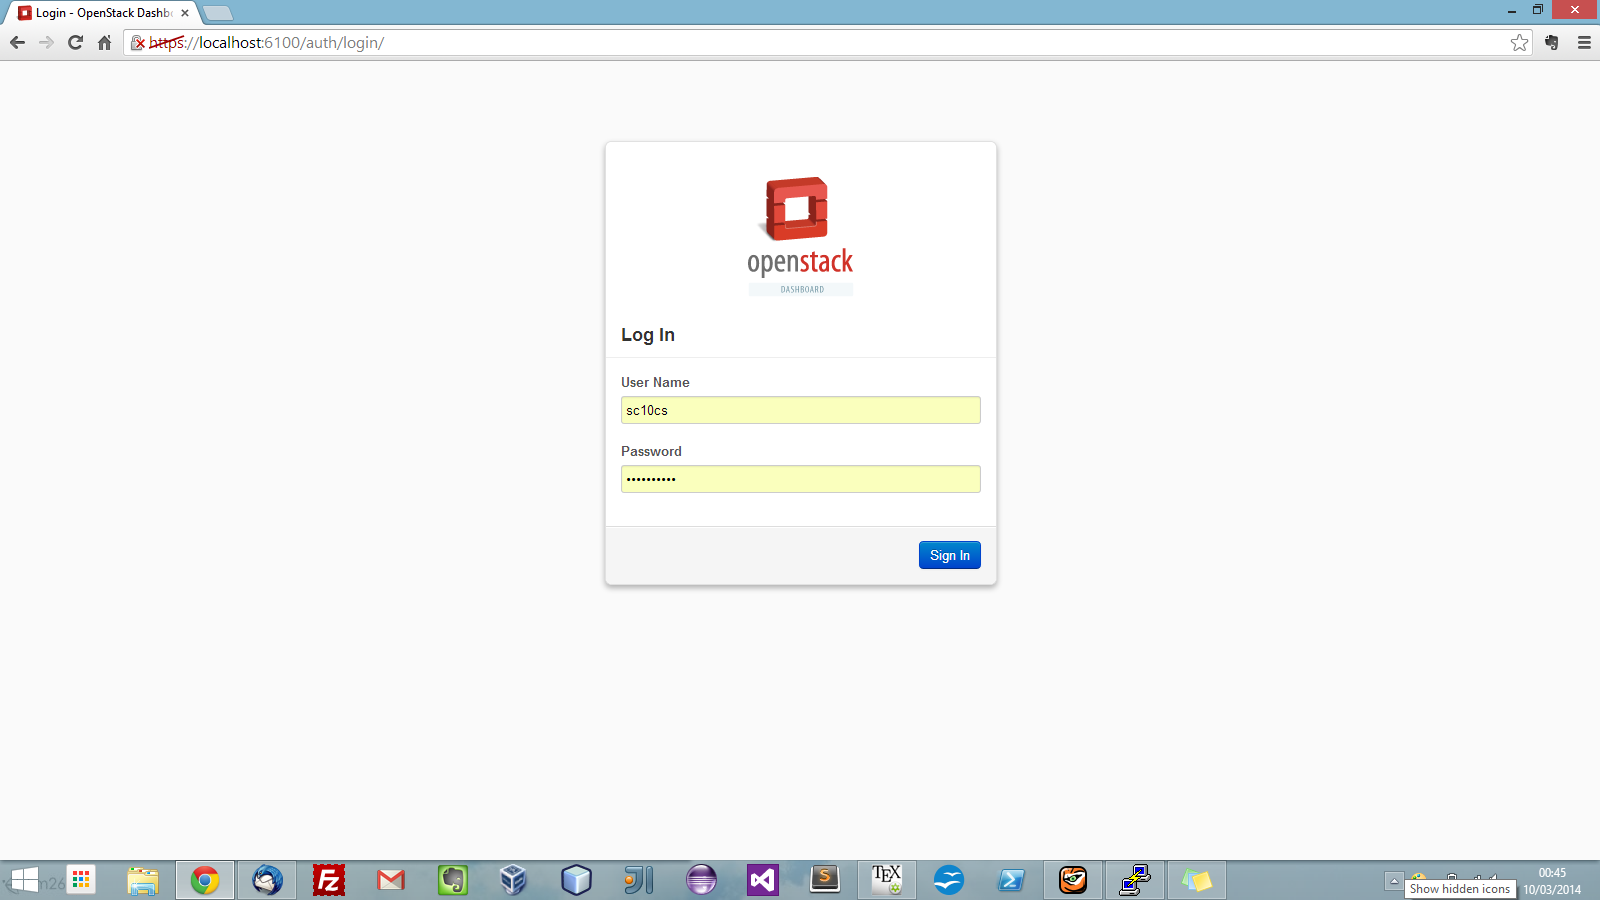
\includegraphics[scale=0.23]{openstack-login}}
\caption{OpenStack Login Screen}
\end{figure}  

\textbf{Step 2: Navigating to the Instance Management View} - Navigating the Dashboard via the various links is very easy, and a good structured view of functionality available. The 'instances' page was accessed by changing project in the 'projects' tag to the sc10cs project, then clicking the 'instances' link on the side panel shown in the below screenshot, which displays the instance management page.
This page contains a navigation panel for various cloud management functions, and a panel on the right to display information based on that navigation. In the case of instances, an empty list of instances with certain information and search functionality can be seen.  
\begin{figure}[H]
\centering
\fbox{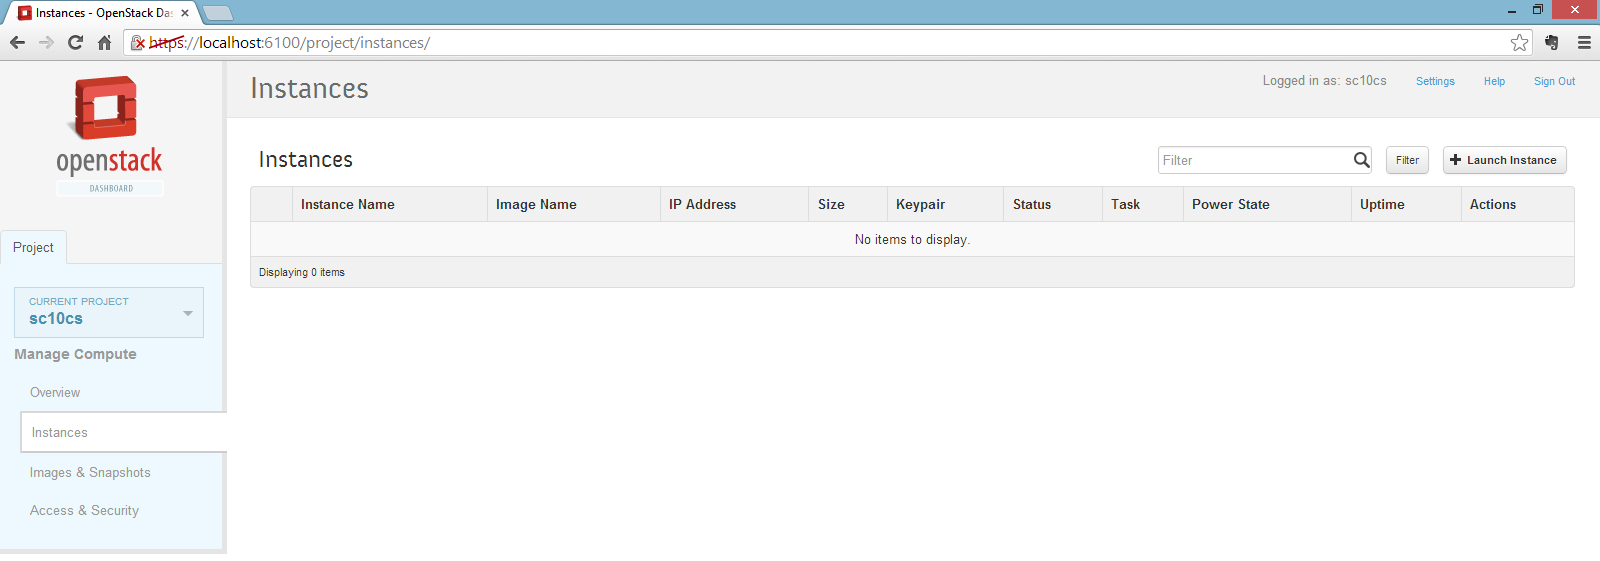
\includegraphics[scale=0.3]{openstack-project-instances}}
\caption{OpenStack Instance Management View}
\end{figure} 
 
\textbf{Step 3: Creating \& Launching an Instance} - The Dashboard UI continues to be very intuitive, and upon clicking the 'Launch Instance' button in the top right of the page, a specialised Instance creation dialog is displayed, shown below. 
\begin{figure}[H]
\centering
\fbox{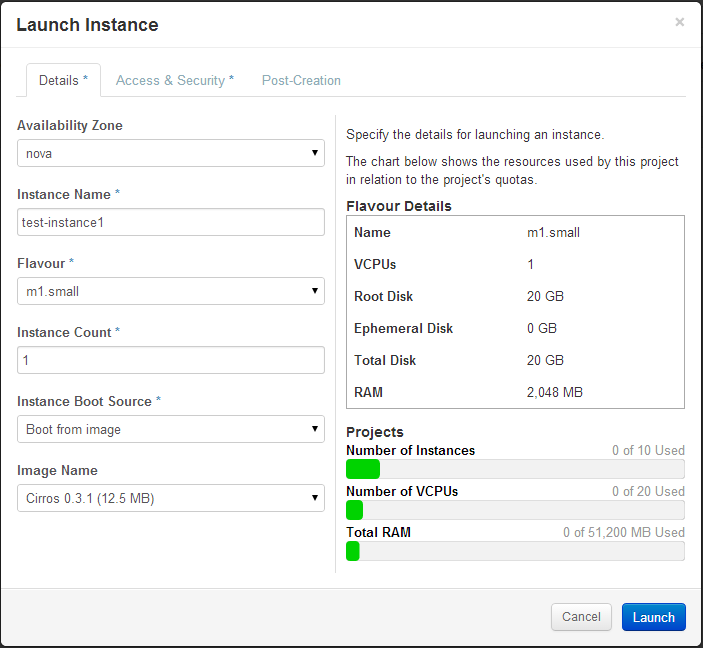
\includegraphics[scale=0.4]{launch-instance-dialog}}
\caption{OpenStack Launch Instance Dialog}
\end{figure}

This dialog allows the user to create a new instance by giving a 'flavour' i.e. a VM size, how much of each resource to allocate to it, and an Image/Snapshot, which act as templates containing deployed software information - these will allow a new instance to be automatically installed and configured by openstack. More options are available in terms of permissions and running post-install scripts. \\

\textbf{Step 4: Checking the Status of the Instance} - Once the launch has been completed, the Web UI almost instantly displays this in the Instances View. Here, certain information can be seen about the instance, including its running status, shown in the below figure:
\begin{figure}[H]
\centering
\fbox{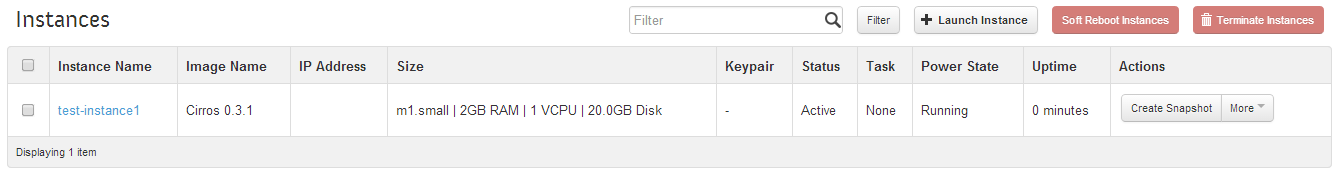
\includegraphics[scale=0.35]{instance-launched}}
\caption{OpenStack Launched Instance}
\end{figure}

\textbf{Conclusion} - 
The Dashboard appears to be an incredibly useful tool. It allowed for quick \& easy authentication through a basic login screen, and simple execution of the task of launching an instance. This tool would be useful for inexperienced users, as it gives a good view of OpenStack functionality, and is very easy to use. Another benefit of the Web Based approach is accessibility; it can be accessed from anywhere with access to the testbed network without logging into the OpenStack machine itself. The main disadvantage of this approach is of course its manual nature - complex tasks may not be suited as they would involve a lot of pointing and clicking. It is my opinion that for my experimentation, smaller, proof of functionality tests would be well suited to execution through the Dashboard.  

\section{Command Line Interface (CLI)}

OpenStack offers a number of Command Line Interfaces, one for each project, which can be used to execute many tasks including Cloud Management \& Information gathering. As the name suggests, this interface to OpenStack is achieved on the Command Line, using a terminal, and using SSH to log directly into the OpenStack machine, testgrid12. The experiment in question will involve use of two main projects, keystone for authentication and the nova for launching an instance. The correct commands must be discovered \& executed in a script, which is provided in this section. To gain a working knowledge of the Command Line Clients associated with OpenStack, I used the official command line reference\cite{openstackcli}.

\textbf{Step 1: Configuring the API Client} - Before any work on the command line could begin, an OpenRC file with information allowing API access was needed. This was accessed through the Dashboard, in the sc10cs project, under Access \& Security -> API access. This file was transferred to the sc10cs account on the OpenStack machine testgrid12 and sourced. It supplies a number of credentials and environment variables which allow access to the CLI. This file is shown below. \\

\begin{figure}[H]
\centering
\fbox{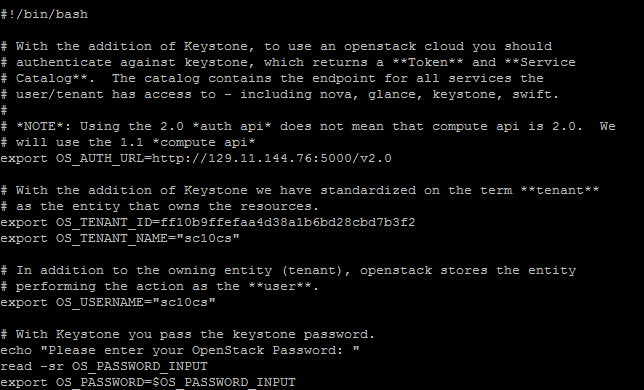
\includegraphics[scale=0.4]{openstackrc}}
\caption{Openstackrc file generated by Dashboard}
\end{figure}


The idea of using a file such as this is that it skips the authentication step of the client process. This information is then readily available to the sc10cs account on testgrid12, and credentials are implicitly included in every command. This greatly simplifies the process of interacting with OpenStack.
The fact that I found this file easy to find out about is a testament to the quality of the official documentation surrounding OpenStack - the information was readily available and easy to access for someone trying to use the CLI.
 \\

\textbf{Step 2: Launching an Instance }- To launch an instance, the nova client's boot command was used. Example boot command usage is as follows:
\begin{figure}[H]
\centering
\fbox{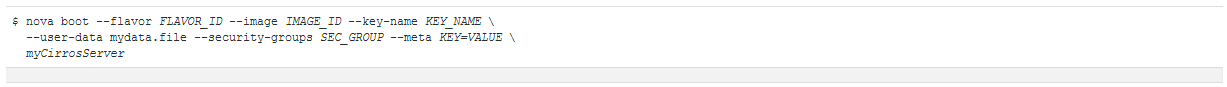
\includegraphics[scale=0.4]{nova-boot-usage}}
\caption{Nova boot usage example}
\end{figure}

In order to use this command effectively, there was a process of using the nova client to obtain certain information about the current system. For example, to find the '\textit{FLAVOR\_ID}', a list of flavors was needed, achieved through using the command '\textit{nova flavor-list}'. The process of obtaining this information as well as image template info and using this to launch an instance is shown below. A scripted version of this is available at the end of this Appendix. The result of the command, shown below, is a table containing status information about the booting instance. 

\begin{figure}[H]
\centering
\fbox{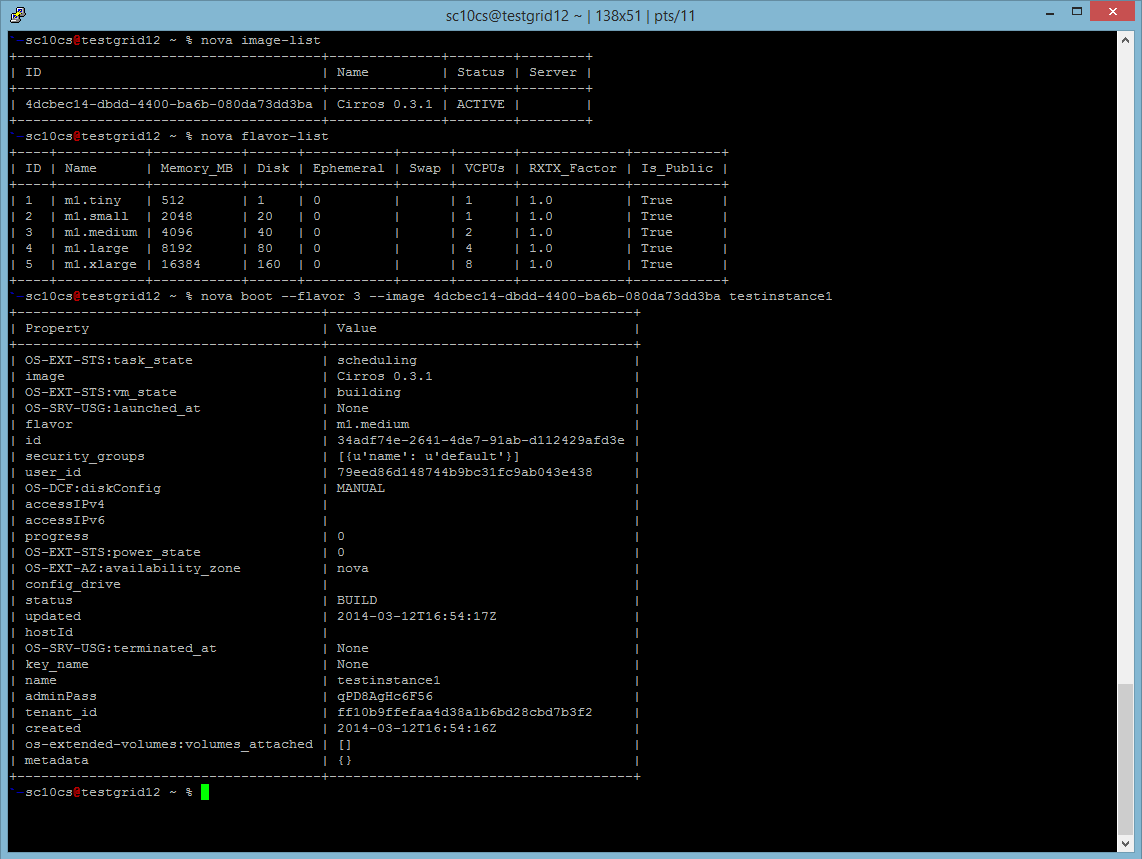
\includegraphics[scale=0.4]{CLI-warmup}}
\caption{Use of Nova to Launch an Instance}
\end{figure}

\textbf{Step 3: Checking the status of the Instance} - Checking up on current images is very simple in the CLI, and only requires one command: \textit{nova list}. The result of this command is a table somewhat similar to the dashboard instances monitor from the first experiment. This table gives the same status information, and is pictured below:
\begin{figure}[H]
\centering
\fbox{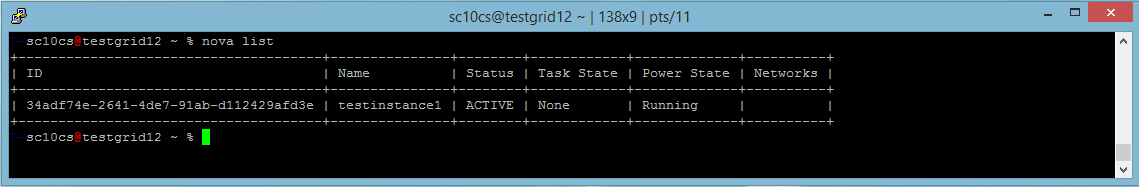
\includegraphics[scale=0.4]{CLI-warmup2}}
\caption{Checking instances with Nova}
\end{figure}

\textbf{Conclusion} - The CLI APIs for OpenStack are a powerful tool. They allow for a wide range of customisation in terms of functionality, and the documentation and response quality surrounding them is of a high standard, meaning that new users could pick them up relatively easily. Another huge advantage of the CLI is the ability to develop automated scripts, especially suited for those tasks which are repeated often and with little variation, for example, a daily status log of instances. This may be useful for some of the practical experiments I plan to execute. There are some obvious disadvantages to this approach, namely the need for configuration of the openrc file and lots of arguments such as tenant\_id which are not intuitive. A second drawback is the need to actually have access to the local OpenStack machine to perform such commands. \\

\textbf{The Script} - The final script of commands used in this experiment to launch and check an instance will be included in my final submission. \\

\section{RESTful Web Service APIs}

RESTful Web Services are APIs exposed over a network through using REST principles. REST, or Representational State Transfer, "\textit{encompasses a simple philosophy for modeling problem domains: “give a URI to everything that can be manipulated by a limited set of operations and let the client software determine the usage metaphor}.”\cite{restoreilly}. Practically, this means each resource is made available with a particular URI, and this is manipulated using HTTP requests which translate to stateless API operations. For example, one may send a POST request with information representing a Server to the server URI \textit{http://openstackint.com/servers}, and this represents the creation of a server. Similarly, sending a HTTP GET request to the same URI may return information about servers. Messages are usually sent in XML or JSON format. More information about REST can be found in the O'Reilly paper on REST\cite{restoreilly}. \\ 

\textbf{Step 0: Setting up Development Environment} - In order to effectively develop experiments using REST Apis, I decided to use the Spring framework\cite{springframework}, an inversion of control framework with REST support, to create clients. This process involved setting up the Eclipse IDE\cite{eclipseide} and using the dependency management tool Maven\cite{maven}. This approach is very popular for REST Clients, although there are alternatives I could have used, such as Jersey\cite{jersey}, which was used in the Distributed Systems Module coursework. 

In order to set up the project, I first installed the Eclipse IDE by downloading a windows executable from \textit{www.eclipse.org}\cite{eclipseide}. Once this was installed, the next step was to create the project. Using Maven, dependencies, such as spring core libraries, are specified in an XML file instead of downloading them manually, and this allows the organised, automated download \& resolution of dependencies at any stage in the development or testing process, e.g. at compile time. An example of one of these files, called \textit{pom.xml}, is shown below. In this project, I used the Spring libraries as well as the Jackson JSON processing library\cite{jackson} for converting Java objects to and from JSON format, the message format used for Openstack's REST APIs.  

\begin{figure}[H]
\centering
\fbox{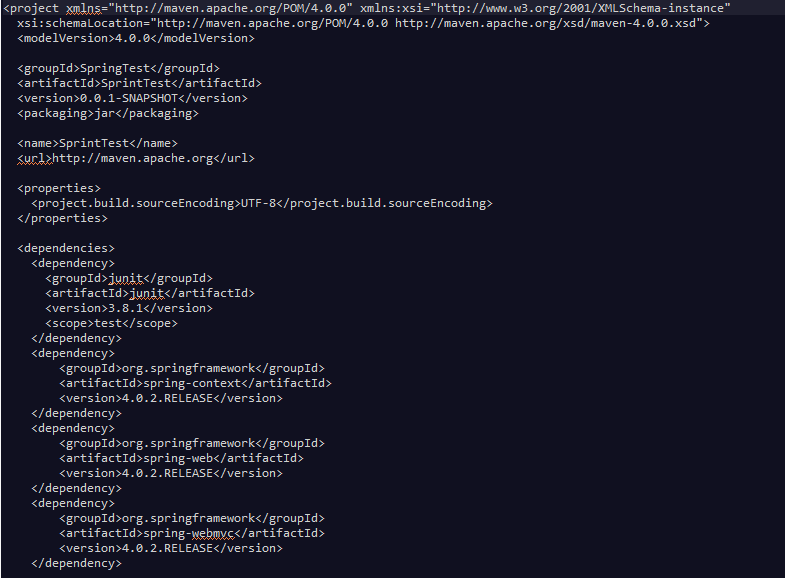
\includegraphics[scale=0.35]{pomxmlexample}}
\caption{Example project pom.xml maven dependency file}
\end{figure}

As part of setting up this project, a lot of research into how the Spring framework, maven \& Jackson work was required. Due to this, the first main point of consideration I noticed was that, although REST clients can be created through basic HTTP request tools in any programming language, to create a professional and effective REST client, i.e. using Spring or Jersey, there is a lot of prerequisite knowledge, compared to using the Dashboard or the CLI. I will briefly introduce the Spring Framework and Jackson in the next steps. \\

\textbf{Step 1: Research Openstack REST APIs} - Before actually developing clients with the tools I had chosen, it was important to first understand the workings of the Openstack REST APIs. For this, I used the official API reference\cite{openstackdocs} along with other sources found on the internet, which will be introduced as they are referenced.  Due to the nature of the first experiment, I focussed on the Keystone \& Nova APIs, as well as formulating a process by which to test out a REST API for further experiments. \\

The first step in accessing an Openstack REST API was figuring out how to actually access the API endpoints, i.e. the Base URL to send requests to. Intuitively I knew that \textit{testgrid12} would be the network resource forming the first part of this URL, accessed over HTTP. From this point, I discovered in the Openstack API refs that a different port is allocated to each service, e.g. Keystone, Nova. One disappointing aspect of the Openstack Documentation is that the port for each service was very difficult to find out, which seems strange as this is vital information. I found the port for each service from scouring the Q \& A board for Openstack\cite{openstackports}, and some of these are displayed below:

\begin{figure}[H]
\centering
\fbox{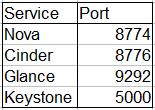
\includegraphics[scale=0.5]{serviceports}}
\caption{Ports for given Openstack services\cite{openstackports}} 
\end{figure}

Once these were accessible, I needed to find a way of sending test requests to these endpoints in order to validate them, and make sure they are functional. Due to requests being made using existing HTTP technologies, there are a number of ways of doing this. For example, a GET request is sent just by putting the URL into a browser's address bar. In this way we can access the keystone API's base URL, which gives API information in response to a GET request, as shown below:

\begin{figure}[H]
\centering
\fbox{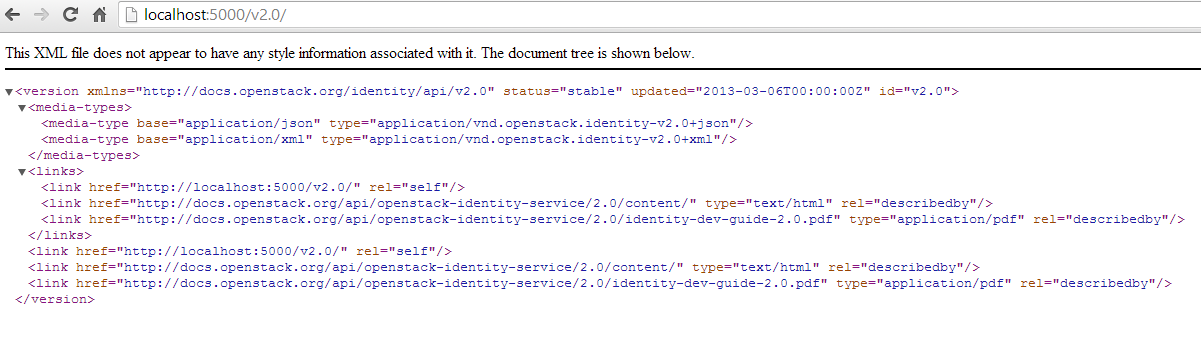
\includegraphics[scale=0.4]{identitybrowserget}}
\caption{Accessing the Keystone Service through a browser} 
\end{figure}

Similarly, the \textit{curl} command can be used to send requests, as shown below: 

\begin{figure}[H]
\centering
\fbox{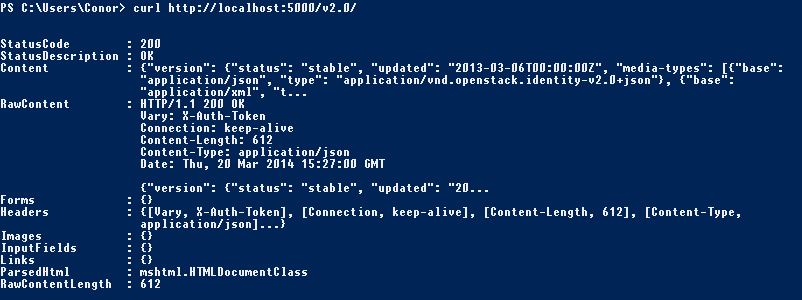
\includegraphics[scale=0.4]{identitycurlget}}
\caption{Accessing the Keystone Service through \textit{curl}} 
\end{figure}

Both of these approaches are valid for basic requests, but for my validation of requests, I used a tool called 'Advanced Rest Client'\cite{advancedrestclient} available as an application on the Google Chrome App Store\cite{googleapps}. This allows for customisation of requests including advanced features such as headers and several message types, including raw JSON. An example of the easy to use Web UI for ARC is shown below: 

\begin{figure}[H]
\centering
\fbox{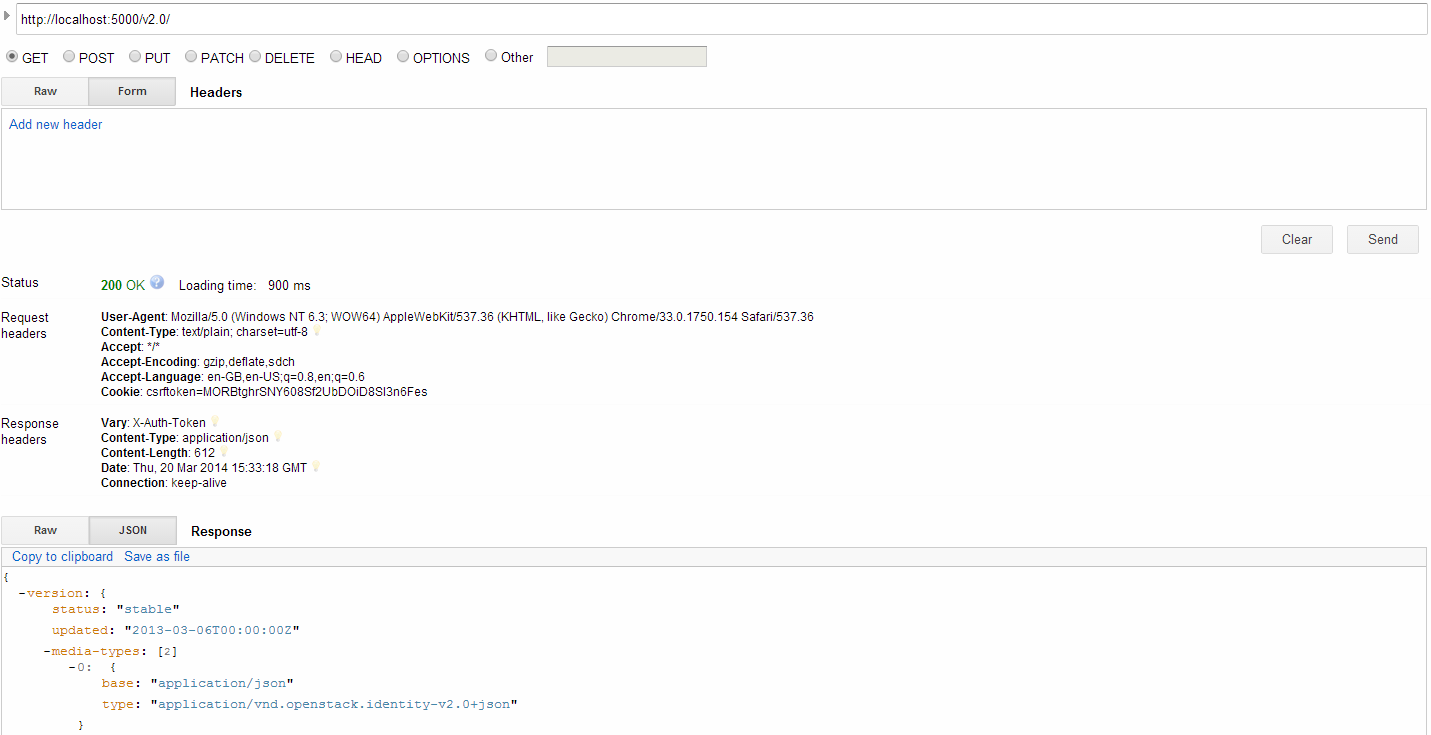
\includegraphics[scale=0.3]{advrestclient}}
\caption{Using Advanced Rest Client to interact with Keystone} 
\end{figure}
 
At this point, I had a way of simulating a rest client to step through the HTTP requests required for the first experiment, as well as the development tools in place to automate the firing of these requests and create a programmatic client. \\

\textbf{Step 2: Developing the Rest Client} - In developing the REST Client for experiments, there were 2 main parts of the work. The first of these was to develop clients for each Openstack service, and some programmatic structure for writing experiments without repeating large parts of the logic in each experiment. Object Oriented Design was used to achieve this goal. Secondly, once the structure of the program was in place, it was time to discern which requests to send to which URIs in order to achieve the aims of the experiment, to launch an instance. Both parts of the work will be described below. \\

\textbf{\textit{Step 2A: Designing \& Implementing Project Structure}} - The structure of the project was based mainly on requirements of the project. The main aspects of the project required were:

\begin{itemize}
\itemsep0em
\item A way of injecting OpenStack configuration (e.g. base uri, ports, user \& password) for different setups. 
\item A way of choosing a number of experiments to run, similar to injecting config files. 
\item A way of easily writing experiments to hook into the experiment runner. 
\item A number of client-side representations of services such as Keystone identity service, to be consumed by experiments. 
\item Some way of reading and writing JSON messages to communicate with REST APIs. 
\end{itemize}

The first requirement, the ability to inject configuration into the application, is something very easily achieved through the use of Spring functionality. Spring allows for XML files to be used to define properties of 'Beans', which are Java Objects with properties determined by these XML files. This is a form of 'Dependency Injection', where values are handed to objects from some outside source, rather than being hard-coded, allowing for less coupled and more flexible applications. For example, in the case of OpenStack configuration, a different XML file can be loaded for different OpenStack installations, users, etc. Every XML bean definition will have a corrsponding class, in this case, \textit{OpenstackConfig.java}, which is populated by the bean definition. These populated objects are loaded into an \textit{Application Context}, through which they can be accessed. The bean definition used for the TestBed can be seen below, along with the corresponding Java class:

\begin{figure}[H]
\centering
\fbox{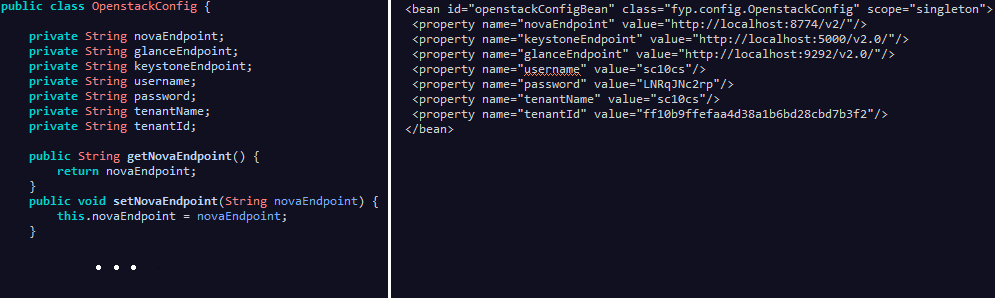
\includegraphics[scale=0.45]{configbean}}
\caption{OpenstackConfig class \& Corresponding Bean definition} 
\end{figure}

Next, to satisfy the requirement to have some way of creating new experiments and a way of running them, I created an abstract class \textit{Experiment}, with the intention that every Experiment would be a subclass of this class, and would need to implement methods to set up, run and tear down the experiment, making it easily executable by a second \textit{ExperimentExecutor} class. Finally, in order to tell the Executor class which experiments to run, a new Bean was defined, based on the java.util.ArrayList class, containing a list of class names for different experiment subclasses. This is loaded into the Application Context by the ExperimentExecutor and each is executed. Below, a class diagram representing what has just been described is shown.

\begin{figure}[H]
\centering
\fbox{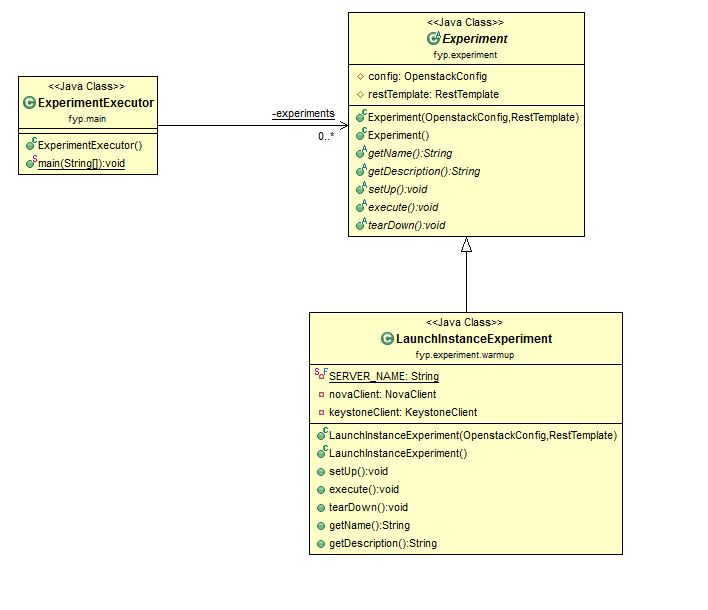
\includegraphics[scale=0.4]{experimentclassdiagram}}
\caption{Class Diagram for Experiment execution} 
\end{figure}

The next requirement, a number of client-side representations of openstack services, was achieved through basic OO abstractions, in the form of interfaces, one for each service, detailing the functionality offered by this service. This is similar to the concept of a proxy class introduced in the Distributed Systems module concerning Java Remote Method Invocation; it is a local version of the functionality which marshals and passes messages. The main difference is that each of these interfaces will be implemented with logic which will perform REST web service interaction with Openstack. The following class diagram demonstrates this use of client interfaces: \\

\begin{figure}[H]
\centering
\fbox{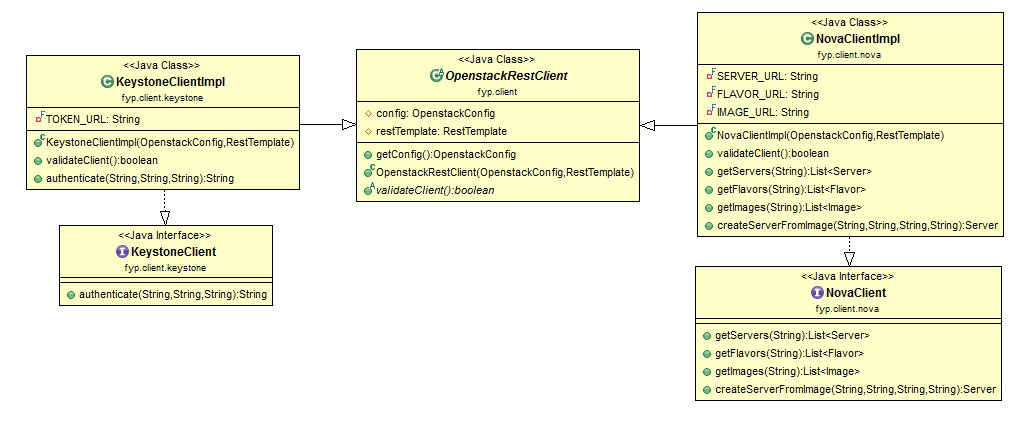
\includegraphics[scale=0.4]{clientclassdiagram}}
\caption{Class Diagram for Openstack clients} 
\end{figure}


Finally, the implementations of the aforementioned interfaces require some way of reading and writing JSON messages to communicate with REST APIs. For this, I used Jackson, a JSON processor with the capability of mapping Java Objects to and from JSON representation. This means that, as long as classes are created to represent data mapping to requests and responses with Openstack, the JSON mapper will implicitly generate and parse JSON. An example of a java class and its JSON counterpart can be seen below.

\begin{figure}[H]
\centering
\fbox{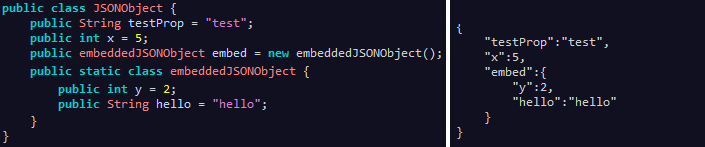
\includegraphics[scale=0.5]{jsonrequestclass}}
\caption{Java request class and mapped Jackson JSON representation} 
\end{figure}

\textbf{\textit{Step 2B: Implementing Experiment Client Functionality}} - In order to execute the first experiment, the correct functionality from both Keystone and Nova clients was needed. The operations required are similar to those required for the CLI experiment, and were researched using the official REST API references for each Service. \\
Firstly, for authenticating with keystone, a POST request to \textit{http://testgrid12:5000/v2.0/tokens} containing user credentials was required, returning a session token to be sent in subsequent requests. To perform REST requests with spring, the \textit{RestTemplate} class is used. A simple call to the \textit{postForObject} method, used in conjunction with the Jackson object mapper, deals with sending and receiving from the Keystone API. The code to do this is shown below:

\begin{figure}[H]
\centering
\fbox{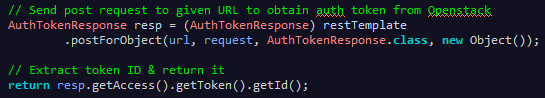
\includegraphics[scale=0.5]{tokenauth}}
\caption{Authenticating a session with Openstack via REST} 
\end{figure}

Once this was authenticated, four more operations were required to be implemented; three of these were relatively simple GET requests to obtain information about which instances, flavors, and images are available. The final operation was a POST request which actually creates and launches a server instance. \\
For any type of request which manipulates openstack resources, an authentication token from the previous request is required. For this reason, the \textit{HttpEntity} class was required as opposed to a simple method representing an HTTP request. An example of this, to create servers, is shown below, encapsulated in a method on the NovaClient interface:

\begin{figure}[H]
\centering
\fbox{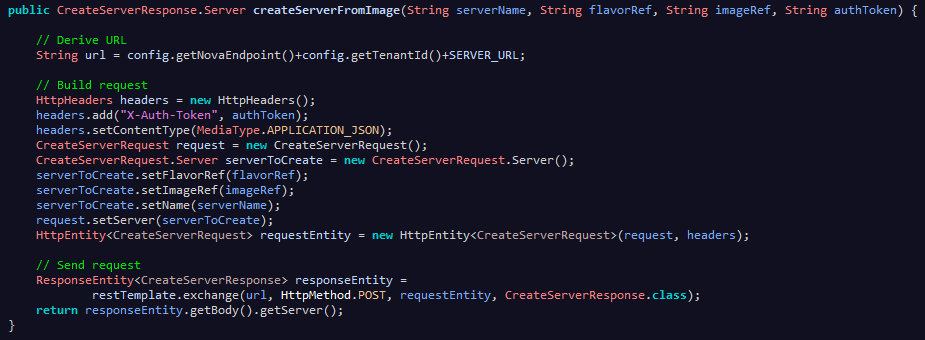
\includegraphics[scale=0.5]{createservercode}}
\caption{Method to create a server on Openstack via REST} 
\end{figure}

Once this was completed, the Experiment could be written. The experiment consists of a number of steps. Firstly, servers, flavors and images are listed from the server. Next, a server instance is created. Servers are then retrieved again, to ensure that launching the instance was actually successful. The code for executing this experiment is shown below. 

\begin{figure}[H]
\centering
\fbox{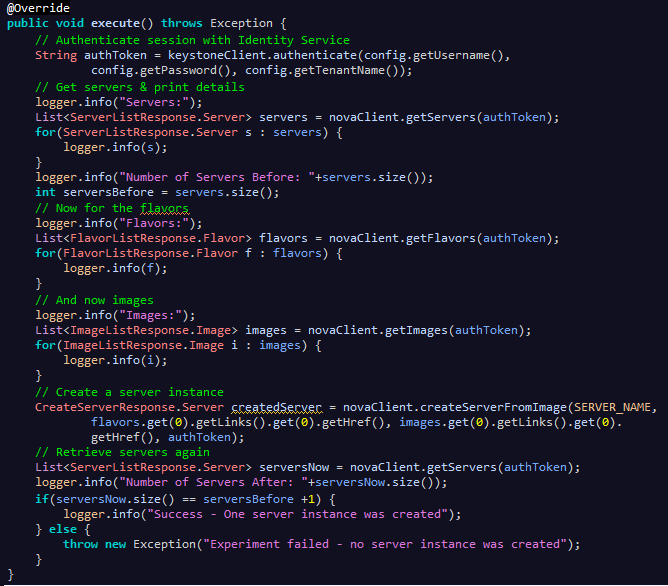
\includegraphics[scale=0.5]{launchinstanceexecute}}
\caption{Experiment to Launch an instance via REST} 
\end{figure}

\textbf{Step 3: Executing the Experiment, Logging results}

Executing the experiment was performed from Eclipse, simply by choosing the option to 'Run as Java Application'. To log results, the Apache Logging tool Log4j was used\cite{log4j}. In the Log4j properties file, included in the submission accompanying this project, a log file is specified to write to as well as to the Eclipse Console (standard output). The output to this log file, from running the experiment, is shown below:

\begin{figure}[H]
\centering
\fbox{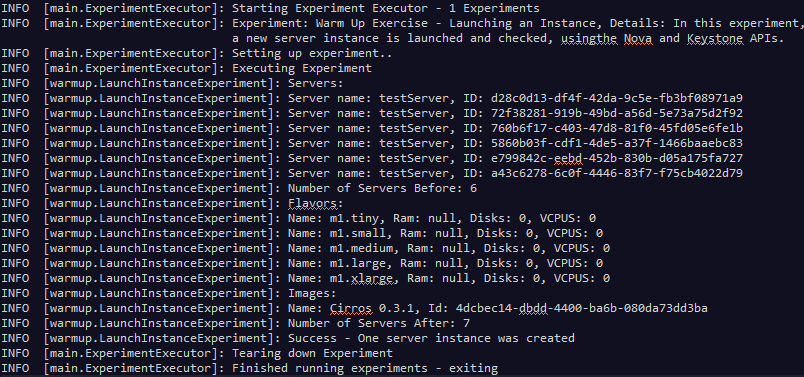
\includegraphics[scale=0.5]{executewarmup}}
\caption{Results of running warmup experiment via REST Client} 
\end{figure}
  
\textbf{Conclusion}  

The OpenStack REST APIs are an incredibly powerful automation tool. They allow the use of Object Oriented principles, or any other structured programming paradigm, through the ability to develop clients in any programming language. This means that clients can be as simple or complex, and similarly as developed as the user wishes. This flexibility makes REST APIs a very useful tool for larger automation tasks, perhaps those which need to be flexible to change and further development, or are complex enough to benefit from the plethora of debugging \& development tools available to modern programming languages.  

One huge advantage of these APIs is the ability to remotely access each individual project on a different port; in the case of the Command line, a direct login to the OpenStack machine is required, and this can cause certain problems with security - in the case of REST, ports can be exposed to easily give access to outsiders. The fact that this runs over HTTP \& HTTPS, very reliable and secure protocols, is an added bonus. 

Another feather in the cap of the REST APIs is the level of documentation available; OpenStack's official docs, referenced in this section, are very informative, and give a good detailed overview of how to use the API. Tools such as the Advanced Rest Client \& curl make testing this out very easy. Each project, being on its own port, is very nicely separated, and it is easy to see from the client side which project or component is being interacted with - useful information for a client considering a change in configuration, for example. 

There are some downsides I spotted from using the REST APIs. Firstly, clients with any real automated capability are rather difficult to develop, and to really get the benefits of REST over, for example, the CLI, a programming language, and not something like curl, should be used. In many languages, due to the need to parse and generate JSON messages, this can get rather complicated, and in the case of Java, means a lot of 'boiler plate code' to map messages to Java objects. \\
Another huge issue I had was the tracking of jobs. Often, when asynchronous jobs are being performed, a Task or Job is returned, allowing the querying of the state of a job. This is not the case for OpenStack as far as my research has shown, and instead, problems can be caused when there are delays to jobs being completed. For example, deleting a Server takes a few seconds after the request has been sent and a response returned, and so if a list of servers is retrieved before this delay, the server will still appear. This of course could cause many automation issues. 
One other issue was with the use of JSON to represent Objects. Often, there would be multiple representations of the same OpenStack 'entity', such as an Image, or a Server. The problem was, in different contexts, different representations of these would be returned, and this can be difficult for a client to handle, without massively overloading the names of objects. Having 4 different 'Server' classes can cause a lot of confusion! An example of this from the provided source code is the class Server.class, and the class ServerInfo.class. ServerInfo is a different representation of a server in OpenStack, providing less information than Server, which is the response from getting all details of a Server, i.e. a 'full' representation.   
 
  
\section{Experiment Conclusion - Comparing Interfaces}

Provided below is a simple table outlining the advantages and disadvantages of each interface to OpenStack, based on my usage of each in this experiment:  

\begin{figure}[H]
\centering
\fbox{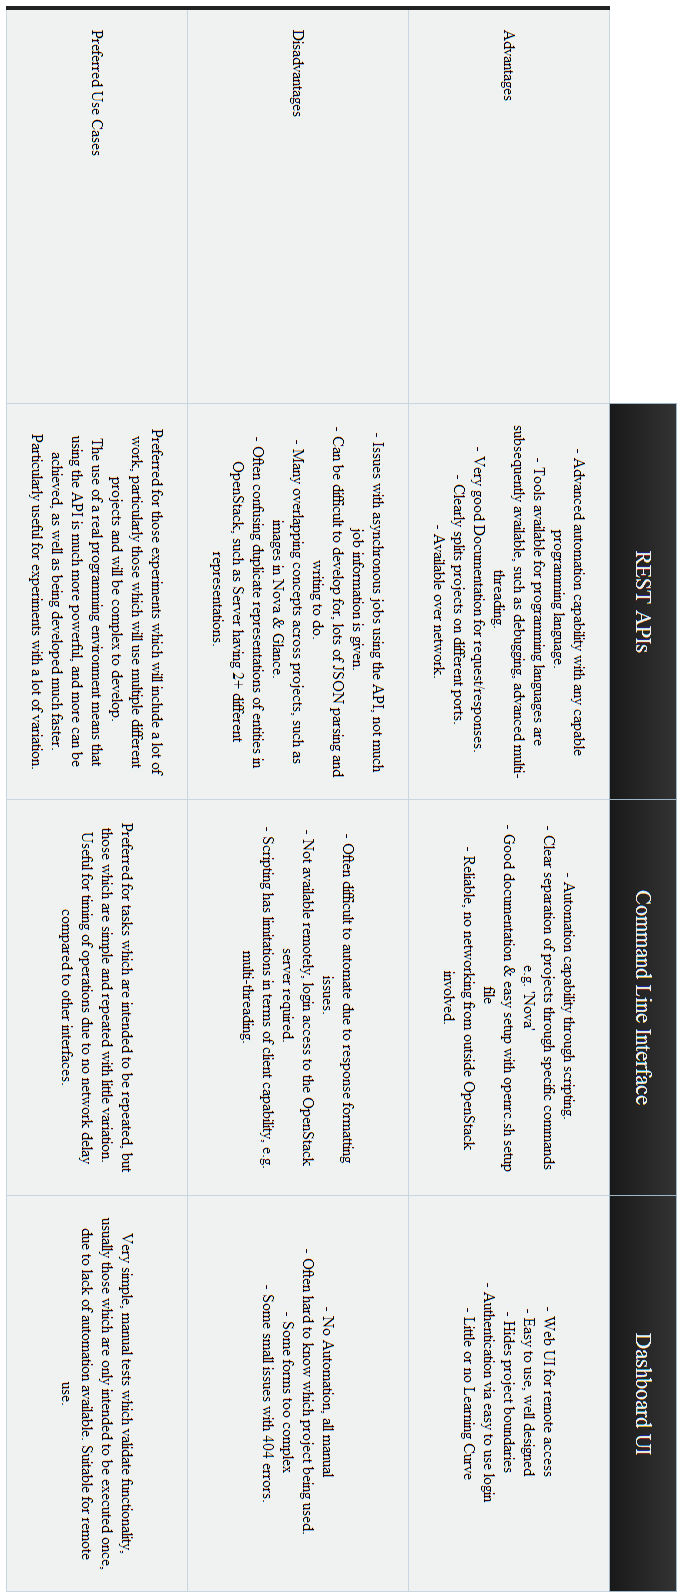
\includegraphics[scale=0.5]{interfacecomparison}}
\caption{Comparison of each interface to OpenStack} 
\end{figure}
\chapter{Project Deliverable - OpenStack REST Client Description}
\centerline{\rule{149mm}{.02in}}
\vspace{2cm}

\section{Introduction}
This appendix aims to give an introduction to the delivered code project called \textit{FYPRestExperiments}. \\
Firstly it will cover how the project is built, which technologies are used, and then will explain the design of the code itself, and in doing so describe how it can be re-used. 


\section{Project Build}

\subsection{Java}
The project uses Java 7\cite{java7}, and is therefore reliant on this version of Java to execute. Due to this, code being developed for this must be written using a Java-compatible technology, such as Java itself or another Java Virtual Machine language like Scala. Similarly, the Java 7 Runtime Environment must be installed in order to execute this application. 

\subsection{Maven}
In order to manage dependencies of the project, such as the Spring Framework\cite{springframework} or Apache's Log4J\cite{log4j} library, the dependency management tool Maven\cite{maven} was used. This tool manages the resolution of dependencies at build, compile or run-time, and simplifies the java build process. \\
Dependencies are stored in XML file in the \textit{pom.xml} file, which defines which software projects will be needed by the current project, including version details. From this, Maven automatically downloads the uses the correct version of the dependency. \\
To use this code for development, for example, using the Eclipse IDE\cite{eclipseide}, as I did in this project, a plugin for maven must be installed, but after this point, the project with dependencies will be built automatically as long as the \textit{pom.xml} file is present. Alternatively, maven can build the project from the command line; more information can be found at the Maven website. \\

By far the simplest way to execute this project is directly from the compiled classes in the main project directory \url{fyprestexperiments}. This can be performed with the \textit{mvn exec:java} command. Arguments can also be passed like so: \textit{mvn exec:java -Dexec.mainClass="fyp.main.ExperimentExecutor" -Dexec.args="test.xml another.xml"} Please ensure you give addresses of xml files relative to the classpath. 

An example of how to run this using maven on the command line is shown below: 

\begin{figure}[H]
\centering
\fbox{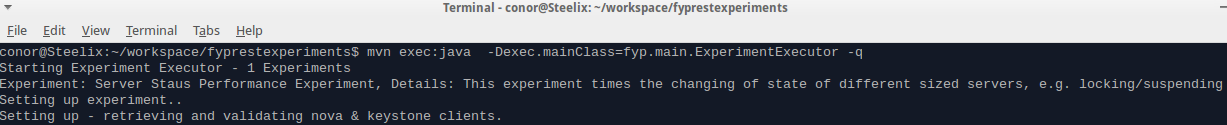
\includegraphics[scale=0.5]{mavenexec}}
\caption{Executing the project with maven on the command line}
\end{figure} 

\section{Project Design}
\subsection{Spring}
The use of Spring has been described briefly in the warm up exercises Appendix (D). The main uses of Spring have been: 
\begin{itemize}
\item Dependency Injection through Java Bean Config
\item Rest Template 
\end{itemize}

The idea behind using Springs JavaBean definition functionality was to allow other users to create their own XML files with their own OpenStack configuration and experiments to execute, meaning that the experiment framework and clients could be easily configured to work anywhere. \\

This project will take any number of arguments representing XML files, and will work as long as beans representing the following are available to the main class, (bean name - class):
\begin{itemize}
\item openstackConfigBean - fyp.config.OpenStackConfig
\item experiments - java.util.ArrayList<fyp.experiments.Experiment>
\end{itemize}

examples of each of these being implemented can be found in \url{fyprestexperiments/src/main/java/fyp/beans/Beans.xml} and \url{fyprestexperiments/src/main/java/fyp/beans/Experiments.xml} respectively. \\
As long as these beans are satisfied, the following automatic configuration takes place, thanks to Spring:
\begin{itemize}
\item Each subclass of OpenstackRestClient has access to the openstack config, so it knows where to send requests. 
\item Each subclass of Experiment has access to the config too, so it can pass information on where necessary.  
\item The experiment Executor knows which subclasses of Experiment to run, and has an instance of each one to execute. 
\end{itemize}

In this way, we have a very smooth execution process without any additional configuration. \\

The \textit{RestTemplate}\cite{resttemplate} class provided by Spring is a useful way of sending requests to a remote URL, using isntances of \textit{HTTPEntity}\cite{httpentity}. The biggest advantage of this is the ability to add a custom java object-JSON converter, in this case, Jackson\cite{jackson}. This meant all message translation was implicit and automatic, through creating classes to hold message data such as the \textit{fyp.nova.data.Server} class and specifying this class in the request. This can be seen in any of the client implementation classes.

\subsection{REST Clients}

The rest clients are very straightforward. They all subclass the \textit{OpenstackRestClient} class, which gives them access to the OpenStack configuration details such as login details and endpoints, and for each different type of client there is an interface specifying it's functionality. The class diagram shown in appendix D illustrates this well:

\begin{figure}[ht]
\centering
\fbox{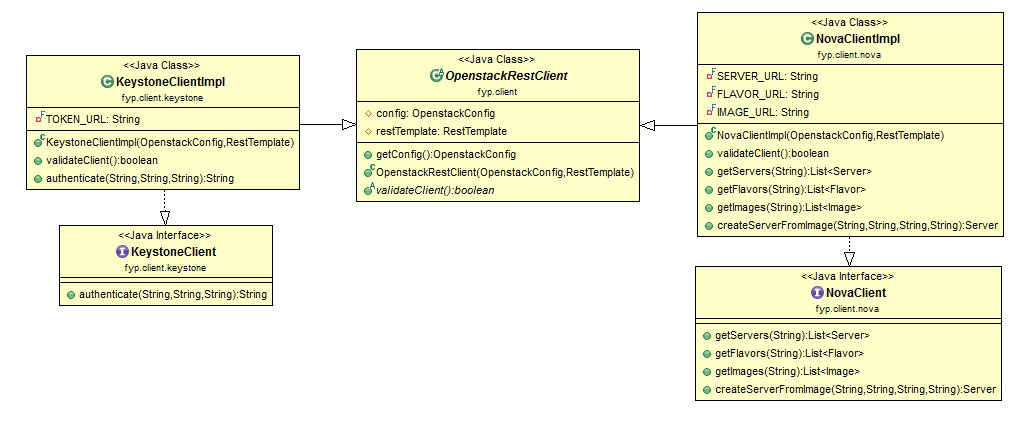
\includegraphics[scale=0.35]{clientclassdiagram}}
\caption{Class Diagram for Openstack clients} 
\end{figure}

These are all implemented to use the aforementioned RestTemplate to send requests based on the information from config and from which interface method is called by an experiment or other client.  \\
The only other piece of configuration concerns the creation of classes to hold request and response information. These can be found in the *.request and *.response packages/directories, and simply allow the jackson JSON converter to match the request or response body to an object. 

\subsection{Experiments}

Experiments were similarly explained in Appendix D. The idea behind writing experiments is to subclass the \textit{fyp.experiments.Experiment} class, providing config automatically, and a number of methods providing the structure of the experiment, such as \textit{setUp}, \textit{execute} and \textit{tearDown}. These methods are automatically called by the main class of this project, \textit{fyp.main.ExperimentExecutor}, and are called for every class defined in the Experiments config bean. 
This class diagram, again from the previous appendix, illustrates this architecture: 
\begin{figure}[ht]
\centering
\fbox{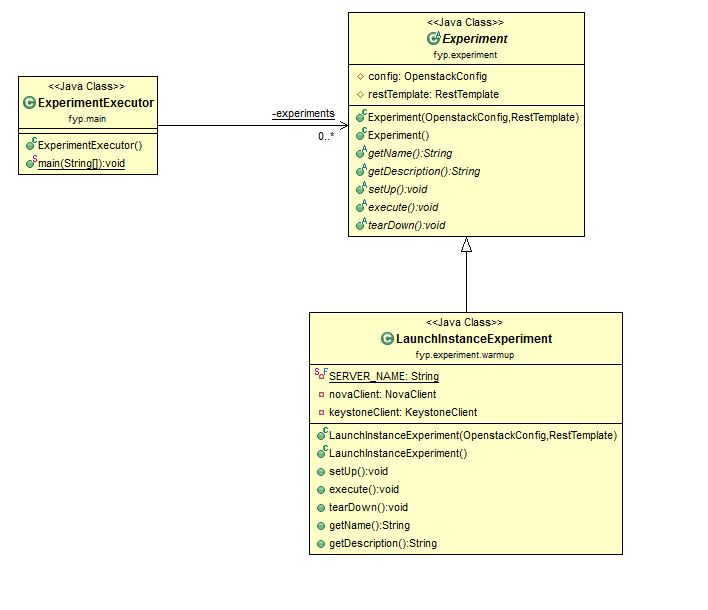
\includegraphics[scale=0.35]{experimentclassdiagram}}
\caption{Class Diagram for Experiment execution} 
\end{figure}

Practically, this means that to create a new experiment to work with this framework, all one needs to do is subclass \textit{Experiment}. 


\subsection{Utilities}

A small number of utilities were added to the project under the \textit{fyp.utils} package, usually to make up for shortcomings of the OpenStack rest apis. These are intended to be used by experiments for convenience, and are designed using static classes. \\

\section{Delivered Items}
The rest client project has delivered the following components: 
\begin{itemize}
\item Source code for a Maven Java project, found under \url{fypexperiments/src/} directory.
\item Compiled source code for execution with Maven \url{fyprestexperiments/target/}
\item A built, executable Jar file containing project code, \url{fypexperiments/target/openstackrestclient-0.0.1-SNAPSHOT.jar}
\item Example Spring Bean config files for reusability, found at \url{fyprestexperiments/src/main/java/fyp/beans/} directory.
\item A number of example experiments to execute or use as a guide found at \url{/home/conor/workspace/fyprestexperiments/src/main/java/fyp/experiment/}
directory.
\item A number of utilities which aid in using the provided rest client interfaces. Utilities: \url{fyprestexperiments/src/main/java/fyp/utils/} interfaces (with implementations): \url{fyprestexperiments/src/main/java/fyp/client/} 
\item logs of each experiment executed, found at \url{fyprestexperiments/logs} directory.
\end{itemize}




\chapter{Initial and final GANTT Chart}
\centerline{\rule{149mm}{.02in}}
\vspace{2cm}

Below are the initial and final GANTT Charts for this project. As you will see, much of the structure of the project remained the same, such as the general flow from research, to implementation, to write-up. One considerable difference in this respect is that each part took much longer than anticipated, meaning there was a little more overlap in tasks, and the project was finished slightly later than expected. \\ 

You will also notice that there is a good deal more planning work in the final schedule, in particular around half way through the project. This has been explained in the Evaluation of this chapter, and comes from the general need for a re-think of the meaning of an 'Evaluation' and the real aims and objectives of the project. \\

Other than these points, the GANTT charts remained very similar, showing that the work in this project was well planned, organised and executed. 


\begin{sidewaysfigure}
\centering
\fbox{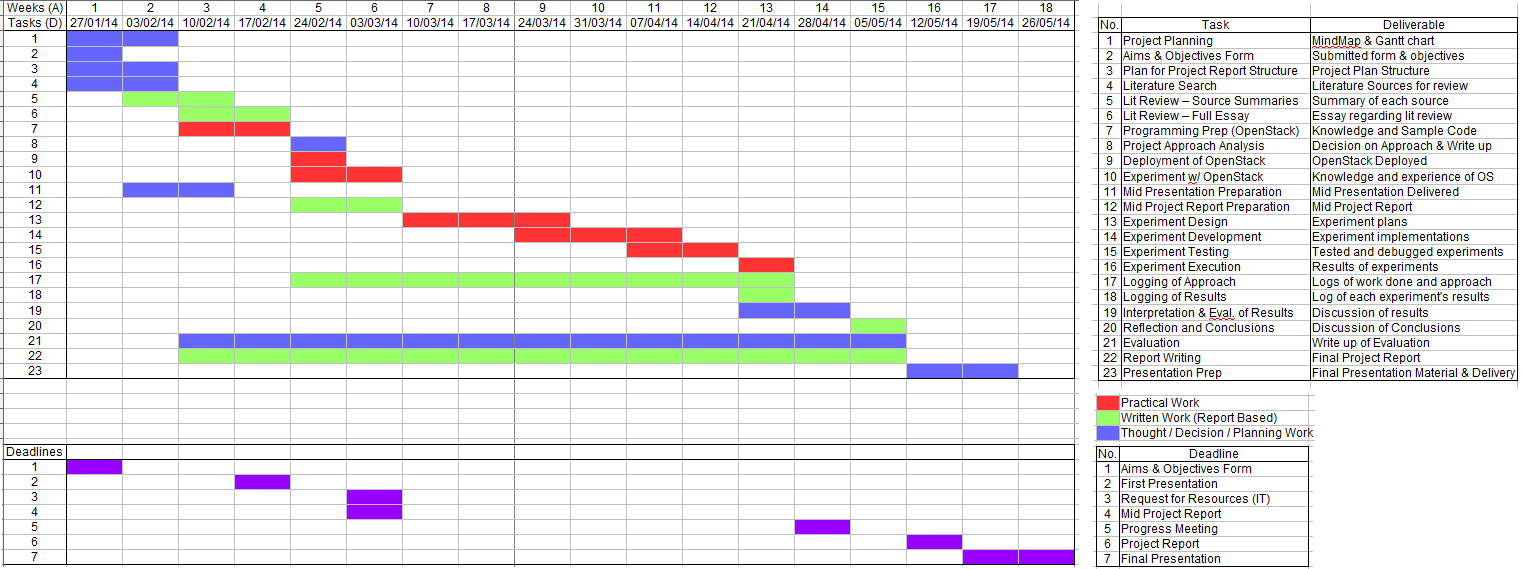
\includegraphics[scale=0.44]{joint-gantts3}}
\caption{GANTT Chart representing initial project schedule \& Deadlines}
\end{sidewaysfigure}



\begin{sidewaysfigure}
\centering
\fbox{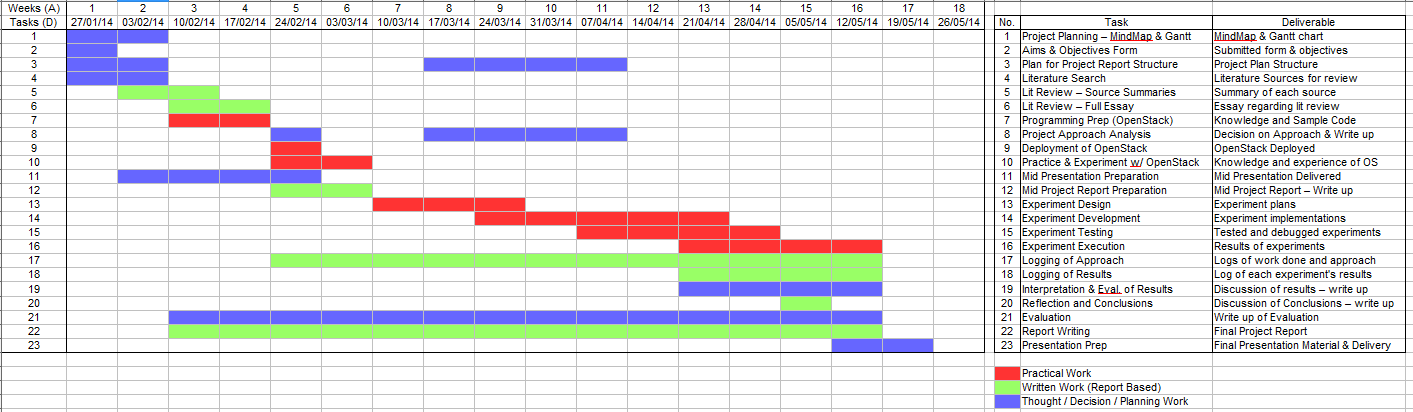
\includegraphics[scale=0.44]{final-gantt}}
\caption{GANTT Chart representing final project schedule}
\end{sidewaysfigure}

\chapter{Mid Project Report}
\centerline{\rule{149mm}{.02in}}
\vspace{2cm}

This project has got off to a good start. From the formulation of the ideas and project plan, to background research, most of the 'preparation' phase of my work, as detailed in the following draft introduction chapter, has been finished. Currently, I am moving on to the practical work required for the 'Implementation phase' of the project. The work I have done so far will be outlined in this section, and provided in full in other sections of this report.\\

\subsection{Part 1: Aims \& Objectives}

The first part of the work I completed was concerned with what the focus of the project would actually be. The title of this project, An Evaluation of OpenStack, left a lot of scope for choice for my approach. These aims \& objectives were decided on in the first week by myself and Karim, based on what we would like to see as an end result for the project, and what we were trying to achieve. The full aims, objectives, minimum requirements, and deliverables have been outlined in the 'introduction' section of this report, along with possible extensions. The basic idea we came up with was to design and execute a number of experiments to assess OpenStack functionality. Part of this was also to justify the project \& outline what it would actually achieve, and this is also covered in the introduction chapter. 

\subsection{Part 2: Project Planning} 
Once the overall aim of the project was decided, the next step was to actually plan the project, from two different perspectives; one from the organisation and scheduling perspective, and one concerning the actual project approach and methodologies I would be using. 

\subsubsection{Project Methodology}

This part of the decision making and planning phase was important to finish first as the actual timetabling of work was dependent on it. This included getting some idea of what work needed to be done, and how it would be approached, including the approach to developing experiments to execute throughout the project. The actual project approach, covered in the introduction chapter, was split into 4 main stages, the first of which includes project planning. Mind maps were also developed, here seen in appendix B, to get an overview of what work was to be done. 

\subsubsection{Project Scheduling}

Once the approach and work to do was decided and written up, I felt it necessary to begin to plan and schedule when certain work would be completed. The first step here was to create a GANTT chart detailing the high level tasks which would need completing, to give some target for each week's achievements. This can be found in appendix B. Similarly, a chart of each project deadline was made to compare this with. So far, this GANTT chart has been strictly adhered to, until very recently, i.e. week starting 03/03/2014, as holdups to the availability of OpenStack on the Cloud TestBed have prevented me from doing any practical work thus far. This could have a knock-on effect for the rest of the project, and so it is likely that a new GANTT chart may be needed, or the original may be deviated from. \\
The next step in this process was to take deadlines and tasks and form a number of milestones to effectively judge the progress of the project; these are detailed in the introduction chapter. 

\subsection{Background Research} 

This has been the main bulk of the work done to date. The literature review and write up, detailed in the Background Research chapter, gives an introduction to the Cloud Computing domain, focusing on the relevant areas to OpenStack, such as Virtual Infrastructure Management \& Infrastructure as a Service clouds. The research focuses on the current OpenStack offering and its competitors, as well as on the desired aspects \& characteristics of a cloud, as well as the challenges they face. The idea behind this is to target experiments at OpenStack in a way which exhibits the desirable characteristics of a cloud, and deals effectively with its challenges, or not as the case may be. The chapter culminates in my overall plan for evaluating OpenStack. 

\subsection{Implementation}

This is the stage I am currently at, and I am currently waiting for access to OpenStack on the testbed. So far however, I have designed one basic experiment which will log in to OpenStack using the identity service, and use the Nove (compute) part of OpenStack to start up a virtual machine. The idea is to perform this experiment with the Command Line Interface, REST APIs, and Web UI of OpenStack so as to compare their effectiveness for basic usage, and to experiment or 'warm up' with OpenStack and its many use cases. I have also began to set up my development environment using Eclipse \& Jersey, which will be documented in the warm-up section of implementation.

\subsection{Next Steps}

Firstly, I will complete my warm-up exercise and have a written comparison of OpenStack's different interfaces. The next step will be to design and implement a number of experiments, then test \& execute them, collect results, and write up the procedure of each experiment with its results. \\
Once this is finished, it will be time to form some conclusions about my results, and come up with some form of evaluation and point of comparison with competitors for OpenStack. \\
Finally, I will evaluate my approach and results, reflecting on the strengths and weaknesses of my approach, and giving some recommendation as to the usefulness of what I have produced, and what it has contributed to its field. 


\end{document}
